        %%******************************************%%
        %%                                          %%
        %%        Modello di tesi di laurea         %%
        %%            di Andrea Giraldin            %%
        %%                                          %%
        %%             2 novembre 2012              %%
        %%                                          %%
        %%******************************************%%

\begin{document}
    \frontmatter
    \begin{titlepage}
    \begin{center}
        \begin{LARGE}
            \textbf{\myUni}\\
        \end{LARGE}

        \vspace{10pt}

        \begin{Large}
            \textsc{\myDepartment}\\
        \end{Large}

        \vspace{10pt}

        \begin{large}
            \textsc{\myFaculty}\\
        \end{large}

        \vspace{30pt}
        \begin{figure}[htbp]
            \centering
            
\includegraphics[height=6cm]{unipd-logo}
        \end{figure}
        \vspace{30pt}

        \begin{LARGE}
            \textbf{\myTitle}\\
        \end{LARGE}

        \vspace{10pt}

        \begin{large}
            \textsl{\myDegree}\\
        \end{large}

        \vspace{40pt}

        \begin{large}
            \begin{flushleft}
                \textit{Relatore}\\
                \vspace{5pt}
                \profTitle\ \myProf
            \end{flushleft}

            % You can tweak the spacing to have professor and student names on the same line
            % useful if the page is broken by a long thesis title and you need more space
            % \vspace{-52pt}

            \begin{flushright}
                \textit{Laureando}\\
                \vspace{5pt}
                \myName
            \end{flushright}
        \end{large}

        \vspace{40pt}

        \line(1, 0){338} \\
        \begin{normalsize}
            \textsc{Anno Accademico \myAA}
        \end{normalsize}
    \end{center}
\end{titlepage}

    \clearpage
\phantomsection
\thispagestyle{empty}

\hfill
\vfill

\noindent\myName: \textit{\myTitle,}
\myDegree,
\textcopyright\ \myTime.

    %\cleardoublepage
\phantomsection
\thispagestyle{empty}
\pdfbookmark{Dedica}{Dedica}

\vspace*{3cm}

\begin{center}
    Lorem ipsum dolor sit amet, consectetuer adipiscing elit. \\ \medskip
    --- Oscar Wilde
\end{center}

\medskip

\begin{center}
    Dedicato a ...
\end{center}

    \cleardoublepage
\phantomsection
\pdfbookmark{Sommario}{Sommario}
\begingroup
\let\clearpage\relax
\let\cleardoublepage\relax
\let\cleardoublepage\relax

\chapter*{Sommario}

Il presente documento descrive il lavoro svolto durante il periodo di stage avvenuto presso l'azienda RiskApp Srl. \\

\noindent Il progetto di stage consisteva nella realizzazione di un'applicazione mobile per la gestione di \gls{meetingnote}\glsoccur, rivolta ad un sotto insieme di utenti che svolgono il loro lavoro in mobilità. \\


\noindent Gli obbiettivi da raggiungere sono stati molteplici. Tra quelli obbligatori erano presenti lo sviluppo della UI e delle funzionalità di base: login, creazione, modifica, eliminazione e visualizzazione di una \gls{meetingnote}\glsoccur.\\
Mentre tra quelli opzionali, l'integrazione di \gls{openai}\glsoccur per automatizzare il processo di creazione menzionato sopra, l'implementazione dei test per la verifica e validazione ed infine l'effettuazione del deploy dell'applicazione sulle piattaforme \emph{Android} e \emph{iOS}.\\

%\vfill

%\selectlanguage{english}
%\pdfbookmark{Abstract}{Abstract}
%\chapter*{Abstract}

%\selectlanguage{italian}

\endgroup

\vfill

    \cleardoublepage
\phantomsection
\pdfbookmark{Ringraziamenti}{ringraziamenti}

\begin{flushright}{
    \slshape
    ``Life is really simple, but we insist on making it complicated''} \\
    \medskip
    --- Confucius
\end{flushright}


\bigskip

\begingroup
\let\clearpage\relax
\let\cleardoublepage\relax
\let\cleardoublepage\relax

\chapter*{Ringraziamenti}

\noindent \textit{Innanzitutto, vorrei esprimere la mia gratitudine al Prof. \myProf, relatore della mia tesi, per l'aiuto e il sostegno fornitomi durante la stesura del lavoro.}\\

\noindent \textit{Desidero ringraziare con affetto i miei genitori per il sostegno, il grande aiuto e per essermi stati vicini in ogni momento durante gli anni di studio.}\\

\noindent \textit{Ho desiderio di ringraziare poi i miei amici per tutti i bellissimi anni passati insieme e le mille avventure vissute.}\\
\bigskip

\noindent\textit{\myLocation, \myTime}
\hfill \myName

\endgroup

    \cleardoublepage
\pdfbookmark{\contentsname}{tableofcontents}
\setcounter{tocdepth}{2}
\tableofcontents
%\markboth{\contentsname}{\contentsname}
\clearpage

\begingroup
    \let\clearpage\relax
    \let\cleardoublepage\relax
    \let\cleardoublepage\relax

    % Figures list
    \phantomsection
    \pdfbookmark{\listfigurename}{lof}
    \listoffigures

    \vspace*{8ex}

    % Tables list
    \phantomsection
    \pdfbookmark{\listtablename}{lot}
    \listoftables

    \vspace*{8ex}
\endgroup

\cleardoublepage

    \cleardoublepage

    \mainmatter
    \chapter{Introduzione}
\label{cap:introduzione}

\intro{In questo primo capitolo viene descritta brevemente l'azienda in cui si è svolto lo stage e l'idea alla base del progetto.}\\

% Introduzione al contesto applicativo.\\

% \noindent Esempio di utilizzo di un termine nel glossario \gls{api}. \\

% \noindent Esempio di citazione in linea \\
% \cite{site:agile-manifesto}. \\

% \noindent Esempio di citazione nel pie' di pagina \\
% citazione\footcite{womak:lean-thinking} \\

\section{Convenzioni tipografiche}
\label{sec:convenzioni-tipografiche}

Riguardo la stesura del testo, relativamente al documento sono state adottate le seguenti convenzioni tipografiche:
\begin{itemize}
	\item gli acronimi, le abbreviazioni e i termini ambigui o di uso non comune menzionati vengono definiti nel glossario, situato alla fine del presente documento;
	\item per i termini riportati nel glossario viene utilizzata la seguente nomenclatura: parola\glsoccur;
	\item i termini in lingua straniera o facenti parti del gergo tecnico sono evidenziati con il carattere \emph{corsivo}.
	\item per i termini salienti negli elenchi puntati viene utilizzato il carattere \textbf{grassetto}.
\end{itemize}

\section{L'azienda}
\label{sec:azienda}

RiskApp Srl è un'azienda, fondata nel 2015 e situata a Conselve (PD) che si occupa di fornire piattaforme digitali per la gestione del rischio nel settore assicurativo.\\
\indent Il core business dell'azienda è quello fornire consulenze e sviluppare software, che attraverso la raccolta e l'analisi di dati, permette di valutare i rischi aziendali. \\
\indent La principale soluzione di punta dell'azienda è la piattaforma \emph{RiskAPP}, composta da diversi moduli, ognuno dei quali è dedicato ad un servizio specifico, alcuni di questi sono:
\begin{itemize}
    \item \textbf{monitoraggio del cliente}\cite{site:riskapp}: attraverso \emph{Cacciatore di Dati}\copyright, una tecnologia proprietaria che si occupa di raccogliere tutte le informazioni disponibili online sul cliente e con l'ausilio di un motore di \gls{iag}\glsoccur è possibile identificare la causa di quello che potrebbe essere un fatto percursore di un sinistro;
    \item \textbf{valutazione delle somme assicurative}\cite{site:riskapp}: una serie di strumenti, permettono di aiutare ad effettuare una corretta valutazione delle somme assicurative, per evitare di incorrere in sovra o sottostime;
    \item \textbf{analisi dei rischi dovuti a calamità naturali}\cite{site:riskapp}: possibilità di prevenire conseguenze negative attraverso la valutazione dei rischi dovuti a calamità naturali;
    \item \textbf{analisi delle esigenze}\cite{site:riskapp}: attraverso lo strumento \emph{Insurance Advisor} è possibile creare un report di consulenza per il cliente, in cui vengono evidenziate le sue esigenze e le possibili soluzioni.
\end{itemize}

\section{L'idea}
\label{sec:idea}

L'idea del progetto di stage è nata dall'esigenza, da parte dell'azienda, di avere uno strumento digitale che permettesse di tracciare gli incontri con i possibili e/o esistenti \glspl{cliente}\glsoccur.
Questi incontri sono molto importanti, in quanto permettono di raccogliere informazioni utili per la creazione di un report di consulenza.\\
\indent Dunque lo scopo finale è quello di avere un'applicazione, integrata nel \emph{Tool trattative}, strumento incluso nella piattaforma \emph{RiskAPP}, che permetta di raccogliere le informazioni più importanti di un incontro in una \gls{meetingnote}\glsoccur, in modo da monitorare il \gls{funnel}\glsoccur di tutte le trattative di una compagnia assicurativa, l'andamento ed eventualmente mettere in atto delle azioni migliorative o correttive in caso di necessità.\\
\indent L'applicazione è rivolta ad un sotto insieme di utenti, i commerciali di una compagnia assicurativa, che svolgono il loro lavoro in mobilità, dunque deve essere usufruibile da dispositivi \emph{mobile}, in particolare gli \emph{smartphone}.\\
Si tratta quindi di sviluppare un'applicazione \gls{crossplatform}\glsoccur, in modo da poter essere utilizzata sia su dispositivi \emph{Android} che \emph{iOS}.

% \section{Organizzazione del testo}

% \begin{description}
%     \item[{\hyperref[cap:processi-metodologie]{Il secondo capitolo}}] descrive ...
    
%     \item[{\hyperref[cap:descrizione-stage]{Il terzo capitolo}}] approfondisce ...
    
%     \item[{\hyperref[cap:analisi-requisiti]{Il quarto capitolo}}] approfondisce ...
    
%     \item[{\hyperref[cap:progettazione-codifica]{Il quinto capitolo}}] approfondisce ...
    
%     \item[{\hyperref[cap:verifica-validazione]{Il sesto capitolo}}] approfondisce ...
    
%     \item[{\hyperref[cap:conclusioni]{Nel settimo capitolo}}] descrive ...
% \end{description}
    \chapter{Processi e metodologie}
\label{cap:processi-metodologie}

\intro{Brevissima introduzione al capitolo}\\

\section{Processo sviluppo prodotto}

    \chapter{Il progetto di stage}
\label{cap:descrizione-stage}

\intro{Nel seguente capitolo viene descritto nel dettaglio il progetto tra cui: gli obiettivi richiesti e la pianificazione del lavoro per la sua realizzazione. Infine viene motivata la scelta di tale progetto.}\\

\section{Descrizione del progetto}
\label{sec:descrizione-progetto}

Lo scopo del progetto stage è quello di sviluppare un'applicazione \gls{crossplatform}\glsoccur per la gestione di \gls{meetingnote}\glsoccur e relativa documentazione.
Nello specifico deve fornire le seguenti funzionalità:
\begin{itemize}
    \item \textbf{creazione} di una \gls{meetingnote}\glsoccur, inserendo le informazioni richieste, essa può avvenire in due modi:
    \begin{itemize}
        \item inserimento \textbf{manuale} dei dati attraverso un \gls{wizard}\glsoccur di creazione;
        \item integrazione con \gls{openai}\glsoccur per \textbf{automatizzare} il processo di creazione.
    \end{itemize}
    \item possibilità di \textbf{modificare} una \gls{meetingnote}\glsoccur già creata, attraverso un \gls{wizard}\glsoccur di modifica, analogo a quello di creazione;
    \item possibilità di \textbf{eliminare} una \gls{meetingnote}\glsoccur dalla lista di quelle create;
    \item \textbf{visualizzazione} di una lista di \gls{meetingnote}\glsoccur, con la possibilità di filtrarla per \gls{cliente}\glsoccur, data e ordine di creazione (dalla più recente o meno recente), inoltre, per ciascuna, è possibile visualizzarne in dettaglio il contenuto;
    \item integrazione con il sistema di \textbf{autenticazione} della piattaforma \emph{RiskAPP}, che può avvenire in due modalità differenti:
    \item \begin{itemize}
        \item inserimento \textbf{manuale} delle credenziali;
        \item tramite \textbf{\gls{riconoscimentobiometrico}}\glsoccur.
    \end{itemize}
    \item possibilità di visualizzare i \textbf{dati dell'utente} autenticato.
\end{itemize}

\section{Obiettivi}
\label{sec:obiettivi}

In questa sezione verranno illustrati gli obbiettivi, definiti nel piano di lavoro, che si prevede di raggiungere durante lo svolgimento del progetto di stage.\\

\subsection{Notazione}
\label{subsec:notazione}

Si farà riferimento alla seguente notazione per indicare il grado di importanza degli obiettivi fissati:
\begin{itemize}
    \item \textbf{O}, identifica i requisiti obbligatori, vincolanti in quanto obiettivo primario richiesto dal committente;
    \item \textbf{D}, identifica i requisiti desiderabili, non vincolanti o strettamente necessari, ma dal riconoscibile valore aggiunto;
    \item \textbf{F}, identifica i requisiti facoltativi, rappresentanti valore aggiunto non strettamente competitivo.
\end{itemize}
Le sigle indicate saranno seguite da una coppia sequenziale di numeri, che identificano univocamente ogni obiettivo.

\subsection{Obiettivi fissati}
\label{subsec:obiettivi-fissati}

Si prevede lo svolgimento dei seguenti obiettivi:
\begin{itemize}
    \item \textbf{Obbligatori}
    \begin{itemize}
        \item \textbf{O01}: implementare un meccanismo di autenticazione attraverso delle chiamate all'\gls{apig}\glsoccur della piattaforma \emph{RiskAPP};
        \item \textbf{O02}: richiamare, attraverso richieste \gls{httpg}\glsoccur, le \gls{apig}\glsoccur per ottenere i dati necessari da visualizzare;
        \item \textbf{O03}: creazione delle \gls{meetingnote}\glsoccur;
        \item \textbf{O04}: compilazione del contenuto delle \gls{meetingnote}\glsoccur in maniera testuale e vocale;
        \item \textbf{O05}: sviluppo della \gls{uig}\glsoccur grafica dell'applicazione;
    \end{itemize}
    \item \textbf{Desiderabili}
    \begin{itemize}
        \item \textbf{D01}: integrazione di \gls{openai}\glsoccur per la creazione automatica delle \gls{meetingnote}\glsoccur;
        \item \textbf{D02}: \gls{deploy}\glsoccur dell'applicazione sulle piattaforme \emph{Android} e \emph{iOS};
    \end{itemize}
    \item \textbf{Facoltativi}
    \begin{itemize}
        \item \textbf{F01}: implementazione dei test per la verifica e validazione dell'applicazione;
    \end{itemize}
\end{itemize}

\section{Pianificazione}
\label{sec:pianificazione}

Di seguito viene riportata la pianificazione delle attività da svolgere durante il periodo di stage, suddivise per settimane.\\

\subsection{Pianificazione iniziale}
\label{subsec:pianificazione-iniziale}

Pianificazione iniziale definita anteriormente al periodo di stage e documentata nel documento \emph{Piano di Lavoro}.\\

\subsubsection{Prima settimana: 24/07/23 - 28/07/23 (40 ore)}
    \begin{itemize}
        \item Incontro con il tutor aziendale per la presentazione dettagliata del progetto e comprensione dei requisiti richiesti;
        \item Visione del \emph{Tool trattative} e delle \gls{apig}\glsoccur, per la comprensione del contesto applicativo;
        \item Formazione sulle tecnologie e strumenti da utilizzare: \gls{dart}\glsoccur.
    \end{itemize}
\subsubsection{Seconda settimana: 31/07/23 - 04/08/23 (40 ore)}
    \begin{itemize}
        \item Formazione sulle tecnologie e strumenti da utilizzare: \gls{figma}\glsoccur e \gls{flutter}\glsoccur.
    \end{itemize}
\subsubsection{Terza settimana: 07/08/23 - 11/08/23 (40 ore)}
    \begin{itemize}
        \item Realizzazione del \gls{mockup} dell'applicazione;
        \item Analisi dei requisiti;
        \item Fase di progettazione dell'applicazione e realizzazione del diagramma UML delle classi;
        \item Stesura della documentazione relativa alle attività di analisi dei requisiti e progettazione.
    \end{itemize}
\subsubsection{Quarta settimana: 14/08/23 - 18/08/23 (32 ore)}
    \begin{itemize}
        \item Inizio sviluppo UI dell'applicazione (\textbf{O05});
        \item Implementazione del meccanismo di autenticazione (\textbf{O01});
        \item Chiamate alle \gls{apig}\glsoccur per ottenere i dati necessari da visualizzare (\textbf{O02});
        \item Stesura dei test per le funzionalità implementate (\textbf{F01}).
    \end{itemize}
\subsubsection{Quinta settimana: 21/08/23 - 25/08/23 (40 ore)}
    \begin{itemize}
        \item Implementazione della funzionalità di creazione delle \gls{meetingnote}\glsoccur (\textbf{O03});
        \item Implementazione della funzionalità di compilazione delle \gls{meetingnote}\glsoccur (\textbf{O04});
        \item Stesura dei test per le funzionalità implementate (\textbf{F01}).
    \end{itemize}
\subsubsection{Sesta settimana: 28/08/23 - 01/09/23 (40 ore)}
    \begin{itemize}
        \item Continuazione sviluppo UI dell'applicazione (\textbf{O05});
        \item Integrazione di \gls{openai}\glsoccur per la creazione automatica delle \gls{meetingnote}\glsoccur (\textbf{D01}).
    \end{itemize}
\subsubsection{Settima settimana: 04/09/23 - 08/09/23 (40 ore)}
    \begin{itemize}
        \item Completamento dello sviluppo UI dell'applicazione (\textbf{O05});
        \item Stesura dei test per le funzionalità implementate (\textbf{F01}).
    \end{itemize} 
\subsubsection{Ottava settimana: 11/09/23 - 15/09/23 (40 ore)}
    \begin{itemize}
        \item Esecuzione dei test per la verifica e validazione dell'applicazione (\textbf{F01});
        \item Stesura della documentazione relativa alle attività di codifica;
        \item \Gls{deploy}\glsoccur dell'applicazione sulle piattaforme \emph{Android} e \emph{iOS} (\textbf{D02}).
    \end{itemize}

% INSERT GANTT CHART
\textbf{INSERIRE DIAGRAMMA DI GANTT}

\subsection{Variazione della pianificazione}
\label{subsec:variazione-pianificazione}

Durante già la prima settimana di stage, si è  effettuato un cambiamento che ha portato ad una variazione della pianificazione iniziale, senza però compromettere il percorso di realizzazione del prodotto e il raggiungimento degli obiettivi fissati.\\
Una prima motivazione di tale variazione è dettata da un consiglio del tutor aziendale di sviluppare un prototipo dell'applicazione, in modo da fornire un notevole aiuto nell'analisi dei requisiti e di conseguenza avere un'idea più chiara di come essa dovrà essere progettata e sviluppata.\\
Inoltre un'altra motivazione, è stata la mia esperienza pregressa, da autodidatta, con il linguaggio \gls{dart}\glsoccur e il framework \gls{flutter}\glsoccur, che mi ha permesso saltare parzialmente parte della fase formativa.\\
Di seguito verranno riportate tali variazioni.

\subsubsection{Prima settimana: 24/07/23 - 28/07/23 (40 ore)}
    \begin{itemize}
        \item Incontro con il tutor aziendale per la presentazione dettagliata del progetto e comprensione dei requisiti richiesti;
        \item Visione del \emph{Tool trattative} e delle \gls{apig}\glsoccur, per la comprensione del contesto applicativo;
        \item Formazione sulle tecnologie e strumenti da utilizzare: \gls{figma}\glsoccur.
        \item Realizzazione del \gls{mockup}\glsoccur dell'applicazione.
        \item Iniziata la fase di analisi dei requisiti dell'applicazione;
    \end{itemize}
\subsubsection{Seconda settimana: 31/07/23 - 04/08/23 (40 ore)}
    \begin{itemize}
        \item Completamento della fase di analisi dei requisiti dell'applicazione;
        \item Formazione sulle tecnologie e strumenti da utilizzare: \gls{dart}\glsoccur e \gls{flutter}\glsoccur;
        \item Iniziato sviluppo  della \gls{uig}\glsoccur dell'applicazione (\textbf{O05}).
    \end{itemize}
\subsubsection{Terza settimana: 07/08/23 - 11/08/23 (40 ore)}
    \begin{itemize}
        \item Completamento dello sviluppo della \gls{uig}\glsoccur dell'applicazione (\textbf{O05});
        \item Fase di progettazione dell'applicazione, ricerca e scelta del \gls{patternarchitetturale}\glsoccur e realizzazione del diagramma UML delle classi;
        \item Iniziato lo sviluppo del meccanismo di autenticazione: inserimento manuale delle credenziali (\textbf{O01});
    \end{itemize}
\subsubsection{Quarta settimana: 14/08/23 - 18/08/23 (32 ore)}
    \begin{itemize}
        \item Completamento dello sviluppo del meccanismo di autenticazione: inserimento manuale delle
        credenziali (\textbf{O01});
        \item Completamento delle funzionalità di ottenimento dei dati da visualizzare attraverso le \gls{apig}\glsoccur (\textbf{O02});
    \end{itemize}
\subsubsection{Quinta settimana: 21/08/23 - 25/08/23 (40 ore)}
    \begin{itemize}
        \item Completamento dello sviluppo della funzionalità di creazione delle \gls{meetingnote}\glsoccur (\textbf{O03});
        \item Completamento dello sviluppo della funzionalità di compilazione delle \gls{meetingnote}\glsoccur (\textbf{O04});
    \end{itemize}
\subsubsection{Sesta settimana: 28/08/23 - 01/09/23 (40 ore)}
    \begin{itemize}
        \item Completamento dello sviluppo del meccanismo di autenticazione: \gls{riconoscimentobiometrico} (\textbf{O01});
        \item Apportati miglioramenti della \gls{uig}\glsoccur per l'ottimizzazione dell'esperienza utente;
        \item Effettuate ottimizzazioni per le performance e refactoring del codice;
    \end{itemize}
\subsubsection{Settima settimana: 04/09/23 - 08/09/23 (40 ore)}
    \begin{itemize}
        \item Impostazione icona e nome dell'applicazione;
        \item Apportati miglioramenti e ottimizzazione del codice;
        \item Commentato il codice e redatta la documentazione relativa alle attività di sviluppo;
        \item Completamento dello sviluppo UI delle viste riguardanti alla creazione automatica delle \gls{meetingnote}\glsoccur  (\textbf{O05});
    \end{itemize}
\subsubsection{Ottava settimana: 11/09/23 - 15/09/23 (40 ore)}
    \begin{itemize}
        \item Completamento dello sviluppo della funzionalità di creazione automatica delle \gls{meetingnote}\glsoccur (\textbf{D01});
        \item Aggiornamento della documentazione relativa alle attività di codifica;
        \item Apportati miglioramenti e ottimizzazione del codice;
    \end{itemize}

È doveroso precisare che, nonostante la fase di progettazione sia avvenuta dopo la codifica della \gls{uig}\glsoccur dell'applicazione e non vicerversa, come previsto nella pianificazione iniziale, ma soprattutto dai principi dell'\gls{ingsw}\glsoccur, non si è andati a compromettere la fase di sviluppo, in quanto si è svolto, la codifica della \gls{uig}\glsoccur, con la consapevolezza di implementare un'architettura che si basasse sul \gls{patternarchitetturale}\glsoccur \Gls{mvcg}\glsoccur, per mantenere una separazione tra la logica di presentazione e la logica di business.\\

% INSERT GANTT CHART
\textbf{INSERIRE DIAGRAMMA DI GANTT}

\section{Motivazione della scelta}
\label{sec:motivazione-scelta}

La scelta di tale progetto è stata dettata da varie motivazioni, tra le quali alcune lo sono di base anche se la decisione fosse stata ricaduta su un qualsiasi altro progetto: ovvero la possibilità di mettersi in gioco e cercare di applicare le conoscenze acquisite durante il percorso di studi, in un contesto più professionale e reale. \\
Inoltre, come menzionato in precedenza, nonostante la mia esperienza pregressa con le tecnologie impiegate, mi ha semplificato la decisione, in quanto avere la possibilità di utilizzarle per sviluppare un progetto in un contesto lavorativo è stimolante e, nonostante mi abbia anche permesso di saltare parzialmente la fase formativa, è stata comunque necessaria per approfondire le conoscenze e acquisirne di nuove.\\
\indent Il mancato soddisfascimento degli obbiettivi \emph{D02} e \emph{F01}, è stato dovuto, in generale, alla mancanza di tempo, in quanto, come si può notare dalla variazione di pianificazione, la fase di sviluppo è stata più lunga del previsto.\\
Nonostante non sono stati progettati e scritti i test per la verifica e validazione dell'applicazione, si è comunque cercato di mantenere un codice pulito e ben strutturato, in modo da facilitare eventuali modifiche e manutenzioni future, anche se come garanzia di qualità non può considerarsi sufficiente.
Si specifica, inoltre, che la verifica delle funzionalità  dell'applicazione è stata effettuata dal tutor aziendale o da altri colleghi, lungo tutto il periodo di sviluppo del progetto, fornendo un \emph{feedback} immediato e permettendo di apportare eventuali modifiche e miglioramenti.\\
Per quanto riguarda il \gls{deploy}\glsoccur, il principale motivo per cui non è stato effettuato, è da imputarsi al fatto che l'utenza a cui è rivolta l'applicazione è molto ristretta, risultava quindi superfluo e non necessario pubblicarla sulle piattaforme \emph{Google Play Store} e \emph{Apple App Store}. Tale decisione è stata presa dal tutor aziendale che ha ritenuto più opportuno pensare ad un modo alternativo per distribuire l'applicazione agli utenti finali.

    \chapter{Analisi dei requisiti}
\label{cap:analisi-requisiti}

\intro{In questo capitolo verranno illustrati e descritti i casi d'uso del sistema applicativo e classificati i requisiti analizzati.}\\

\section{Attori}
\label{subsec:attori}

In questa sezione vengono definiti gli \glspl{attore}\glsoccur che interagiscono con il sistema.

\subsection{Attori primari}
\label{subsubsec:attori-primari}

\begin{itemize}
    \item \textbf{Utente non autenticato}: utente che possiede le credenziali per accedere al sistema, ma non ha ancora effettuato l'autenticazione;
    \item \textbf{Utente autenticato}: utente che ha effettuato l'autenticazione al sistema.
\end{itemize}

\subsection{Attori secondari}
\label{subsubsec:attori-secondari}

\begin{itemize}
    \item \textbf{RiskAPP API}: sistema che fornisce le \gls{apig}\glsoccur del \emph{Tool Trattative} per l'interazione con il \gls{backend}\glsoccur dell'applicazione.
\end{itemize}

\section{Token di autenticazione}
\label{subsec:token-autenticazione}

Per \emph{token} di autenticazione, del quale nel corso del documento si farà riferimento, si intende una stringa univoca che, una volta inserite e validate le credenziali, viene generata dal \gls{backend}\glsoccur e memorizzata dall'applicazione, il cui scopo è quello, oltre al mantenimento dell'accesso al proprio account, di effettuare le richieste \gls{httpg}\glsoccur.\\
Si specifica inoltre che ha una durata di 4 ore, dopo le quali l'utente dovrà effettuare nuovamente l'autenticazione per ottenerne uno nuovo.

\section{Casi d'uso}
\label{sec:usecase}

Per lo studio dei \glspl{usecase}\glsoccur del prodotto sono stati creati degli appositi diagrammi che illustrano le interazioni tra gli \glspl{attore}\glsoccur e il sistema.\\
Ciascun \gls{usecase}\glsoccur viene fornito con una descrizione che ne riporta le informazioni principali, come attori coinvolti, pre e post condizioni, scenario principale ed eventuali scenari secondari.\\
Per questioni di leggibilità, i diagrammi sono stati suddivisi in più parti, raggrupando i \glspl{usecase}\glsoccur che costituiscono una macro-funzionalità oppure specificano in dettaglio un \gls{usecase}\glsoccur del sistema.

\begin{figure}[!h] 
    \centering 
    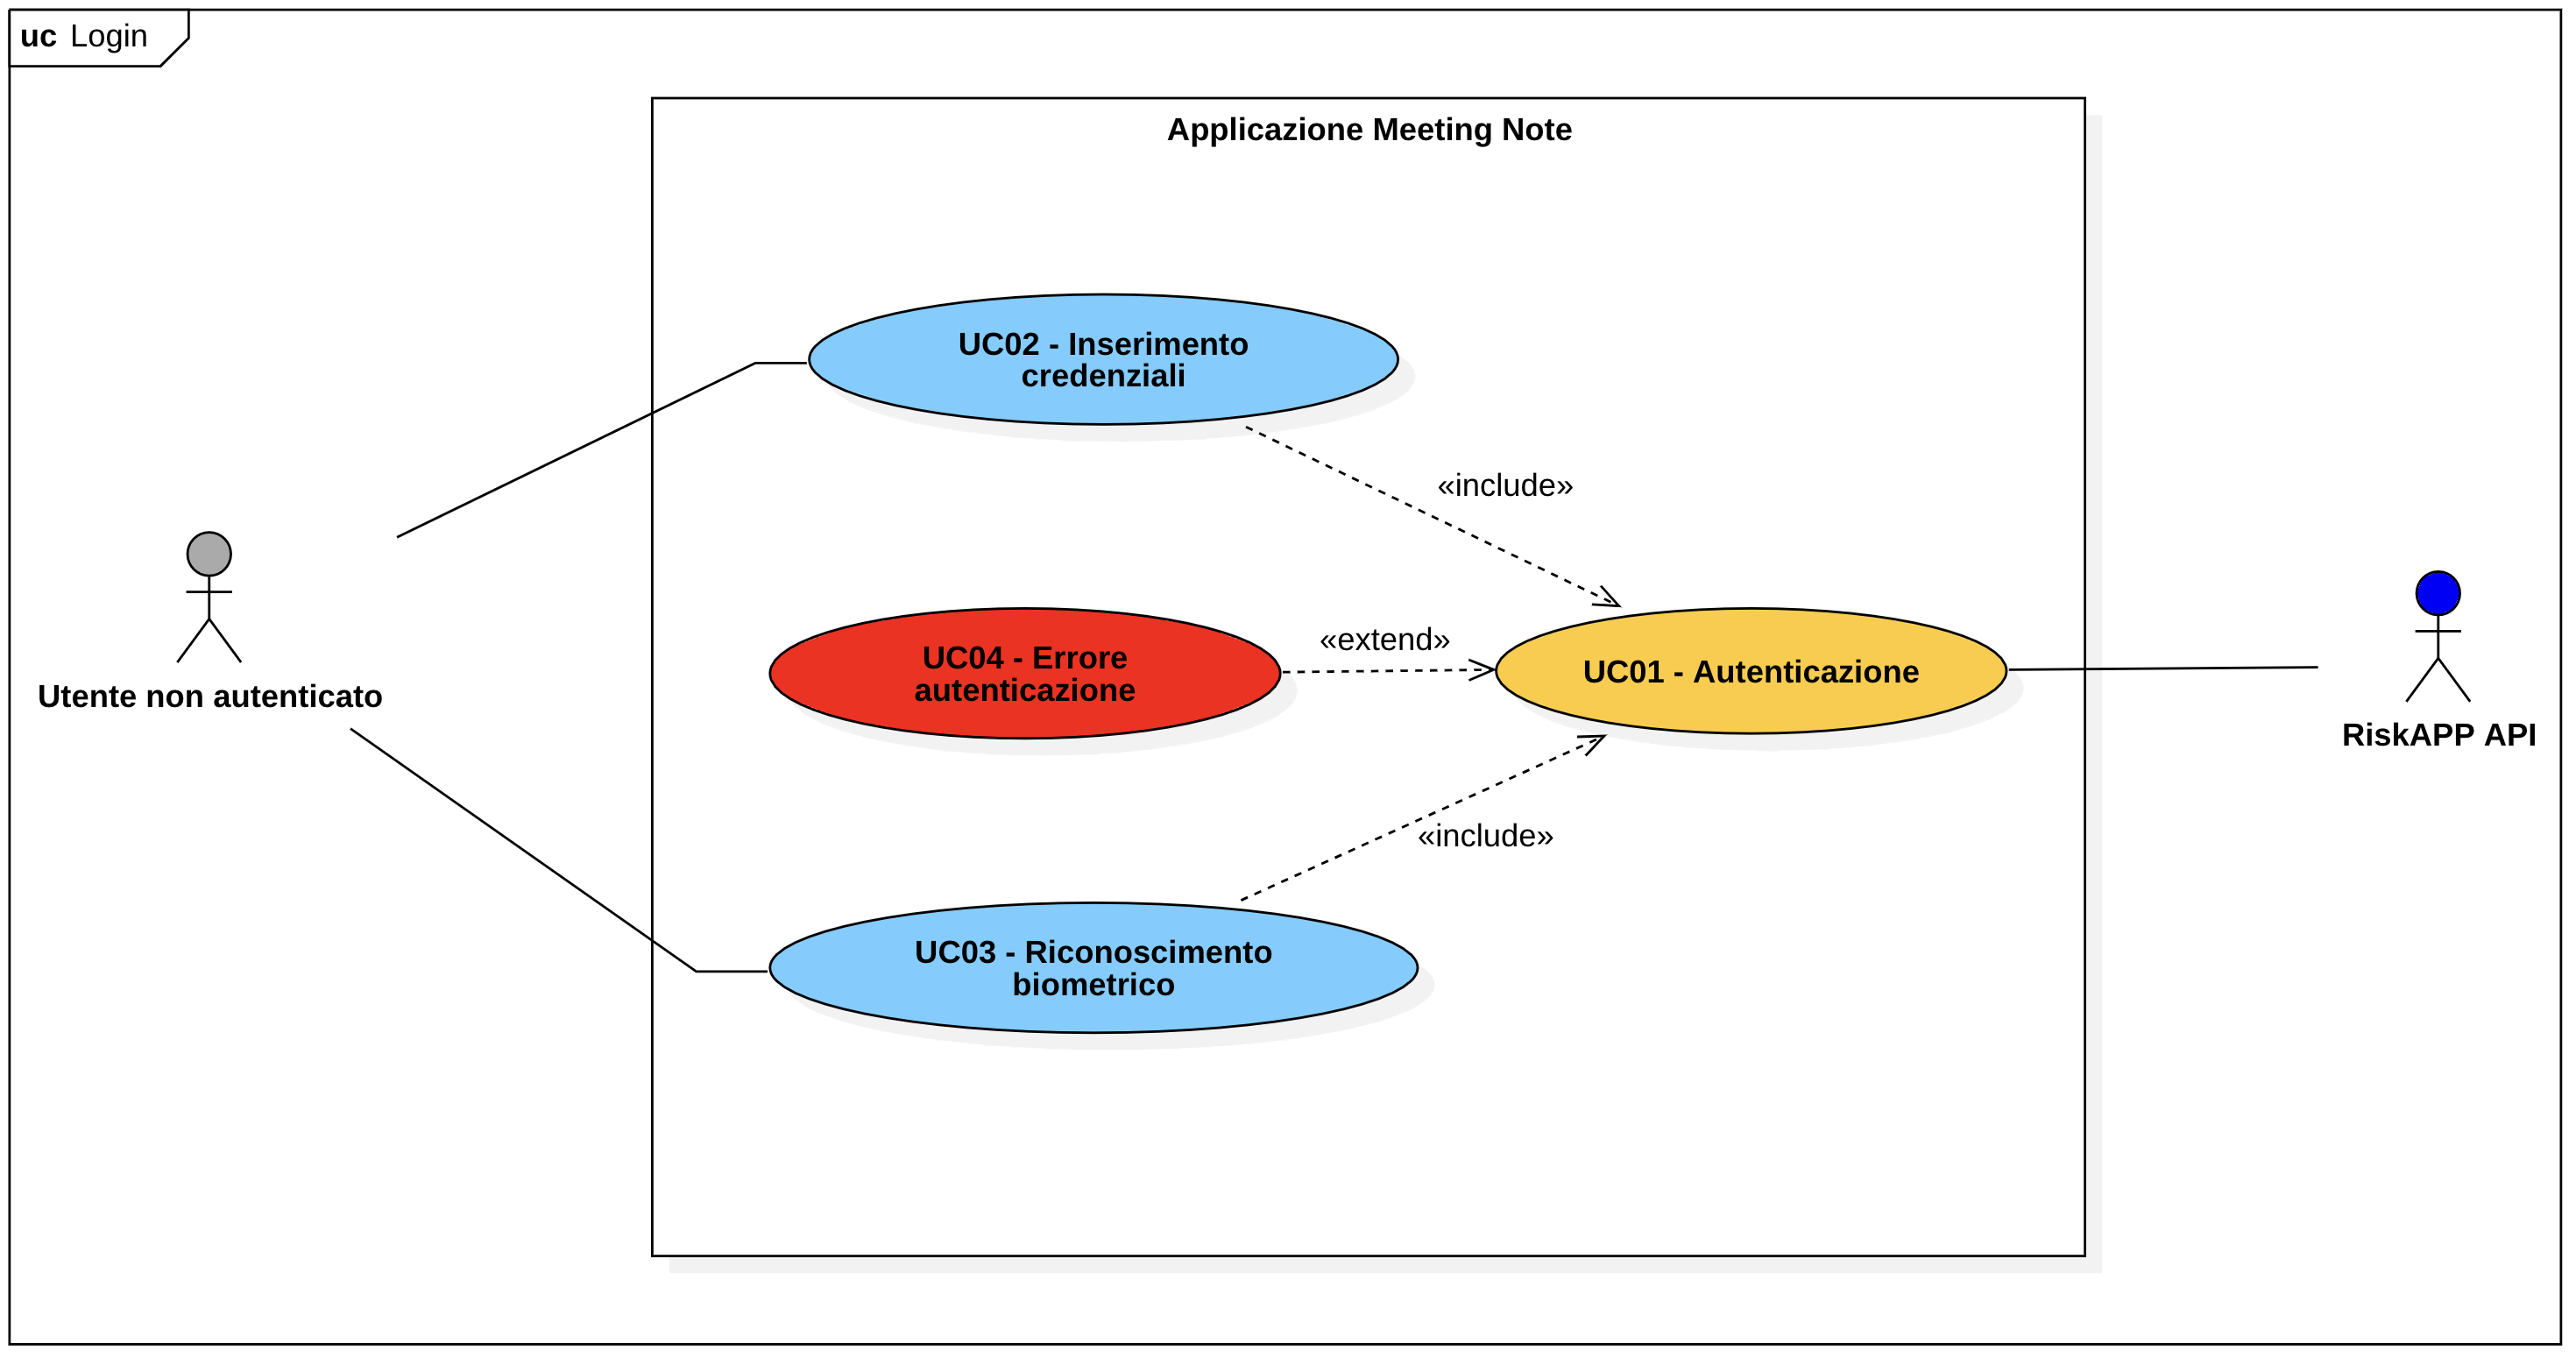
\includegraphics[width=1.0\columnwidth]{usecase/1-uc} 
    \caption{Use Case - Login}
    \label{fig:uc-login}
\end{figure}

\begin{usecase}{01}{Autenticazione}
    \usecasemainactors{Utente non autenticato}
    \usecasesecondaryactors{\emph{RiskAPP API}}
    \usecasepre{L'utente non è ancora autenticato nel sistema}
    \usecasedesc{L'utente effettua l'autenticazione al sistema, scegliendo se farlo, inserendo manualmente le credenziali, oppure tramite \gls{riconoscimentobiometrico}\glsoccur.}
    \usecasepost{L'utente è autenticato nel sistema}
    \usecasealt{Se l'autenticazione fallisce, si verifica \hyperref[UC04]{UC04}}
    \usecaseimg{\ref{fig:uc-login}}
    \label{UC01}
\end{usecase}

\begin{usecase}{02}{Inserimento credenziali}
    \usecasemainactors{Utente non autenticato}
    \usecasepre{L'utente non è ancora autenticato nel sistema}
    \usecasedesc{L'utente inserisce manualmente le proprie credenziali per effettuare l'autenticazione al sistema.}
    \usecasepost{L'utente è autenticato nel sistema}
    \usecaseimg{\ref{fig:uc-login}}
    \label{UC02}
\end{usecase}

\begin{usecase}{03}{Riconoscimento biometrico}
    \usecasemainactors{Utente non autenticato}
    \usecasepre{L'utente non è ancora autenticato nel sistema}
    \usecasedesc{L'utente utilizza il \gls{riconoscimentobiometrico}\glsoccur per effettuare l'autenticazione al sistema.}
    \usecasepost{L'utente è autenticato nel sistema}
    \usecaseimg{\ref{fig:uc-login}}
    \label{UC03}
\end{usecase}

\begin{usecase}{04}{Errore autenticazione}
    \usecasemainactors{Utente non autenticato}
    \usecasesecondaryactors{\emph{RiskAPP API}}
    \usecasepre{L'utente non è ancora autenticato nel sistema}
    \usecasedesc{L'autenticazione fallisce e l'utente viene informato dell'errore; le motivazioni possono essere le seguenti:
        \begin{itemize}
            \item le credenziali inserite non sono corrette;
            \item il sistema non è raggiungibile;
            \item il \gls{riconoscimentobiometrico}\glsoccur è fallito;
            \item connessione ad internet assente.
        \end{itemize}}
    \usecasepost{L'utente non è autenticato nel sistema}
    \usecaseimg{\ref{fig:uc-login}}
    \label{UC04}
\end{usecase}

\begin{figure}[!h] 
    \centering 
    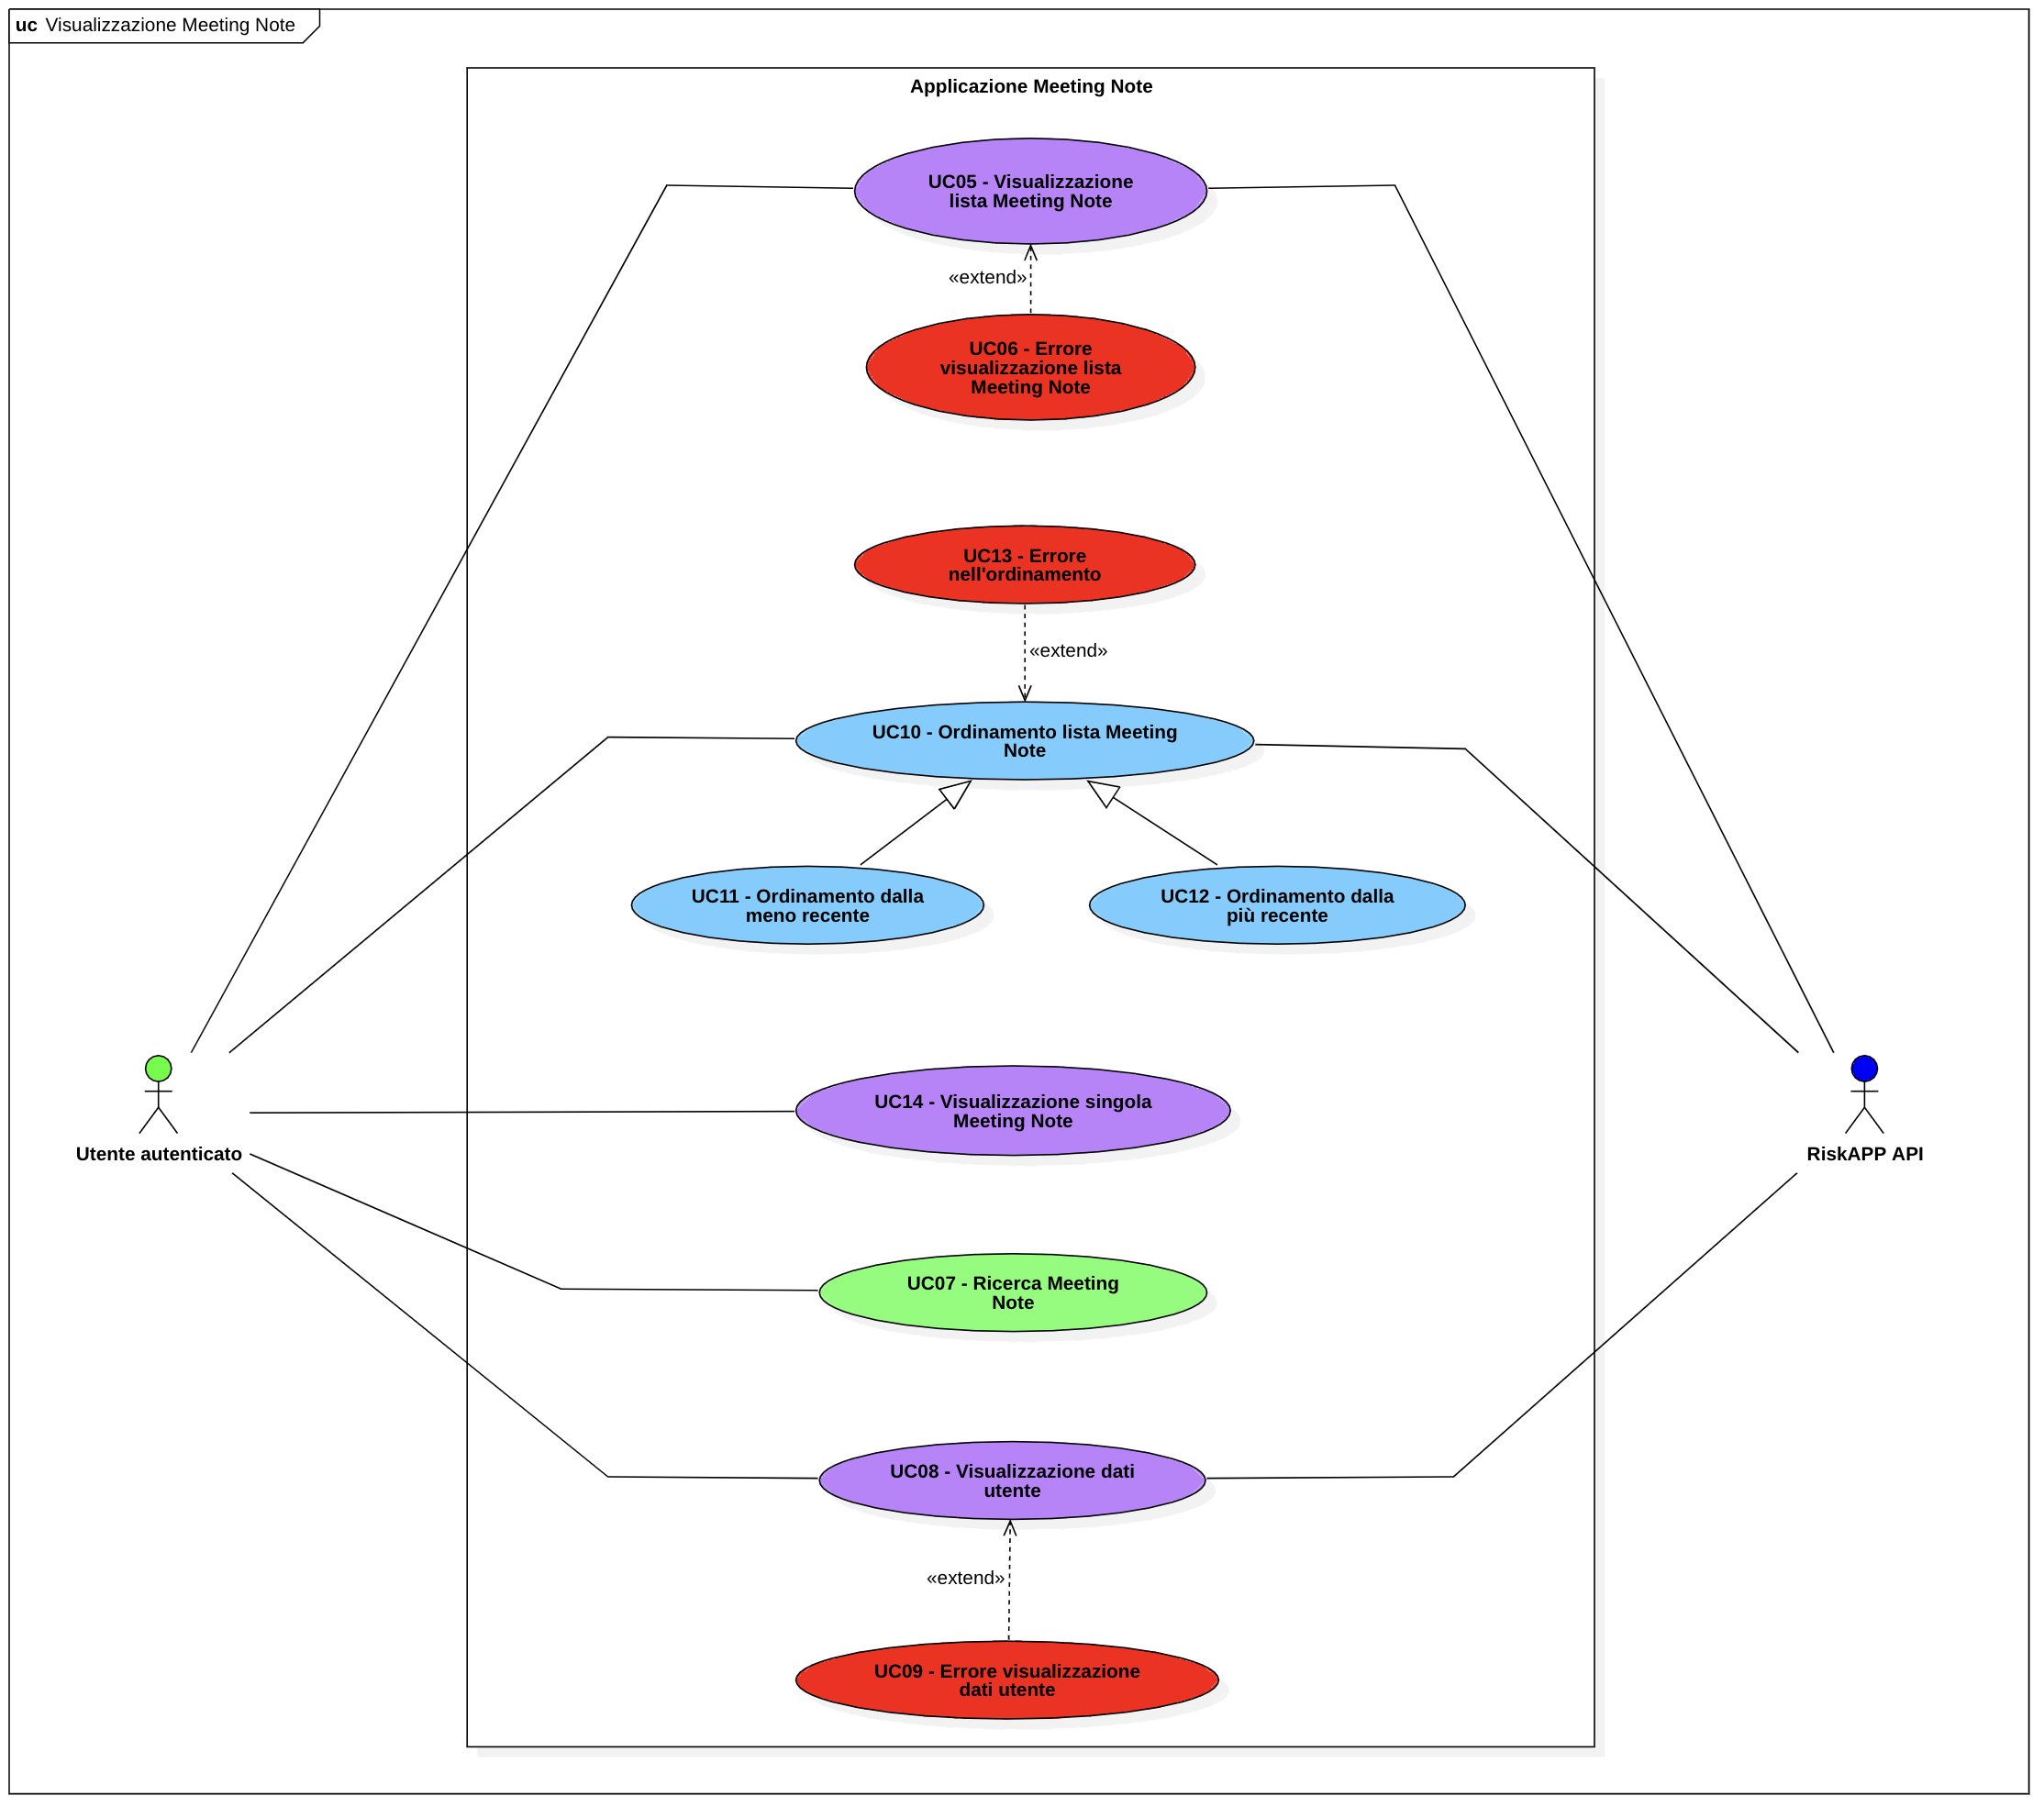
\includegraphics[width=1.0\columnwidth]{usecase/2-uc} 
    \caption{Use Case - Visualizzazione Meeting Note}
    \label{fig:uc-meetingnote}
\end{figure}

\begin{usecase}{05}{Visualizzazione lista Meeting Note}
    \usecasemainactors{Utente autenticato}
    \usecasesecondaryactors{\emph{RiskAPP API}}
    \usecasepre{L'utente è autenticato nel sistema}
    \usecasedesc{L'utente vuole visualizzare la lista di tutte le \gls{meetingnote}\glsoccur associate.}
    \usecasepost{È visualizzabile la lista delle \gls{meetingnote}\glsoccur}
    \usecasealt{Se la visualizzazione fallisce, si verifica \hyperref[UC06]{UC06}}
    \usecaseimg{\ref{fig:uc-meetingnote}}
    \label{UC05}
\end{usecase}

\begin{figure}[!h] 
    \centering 
    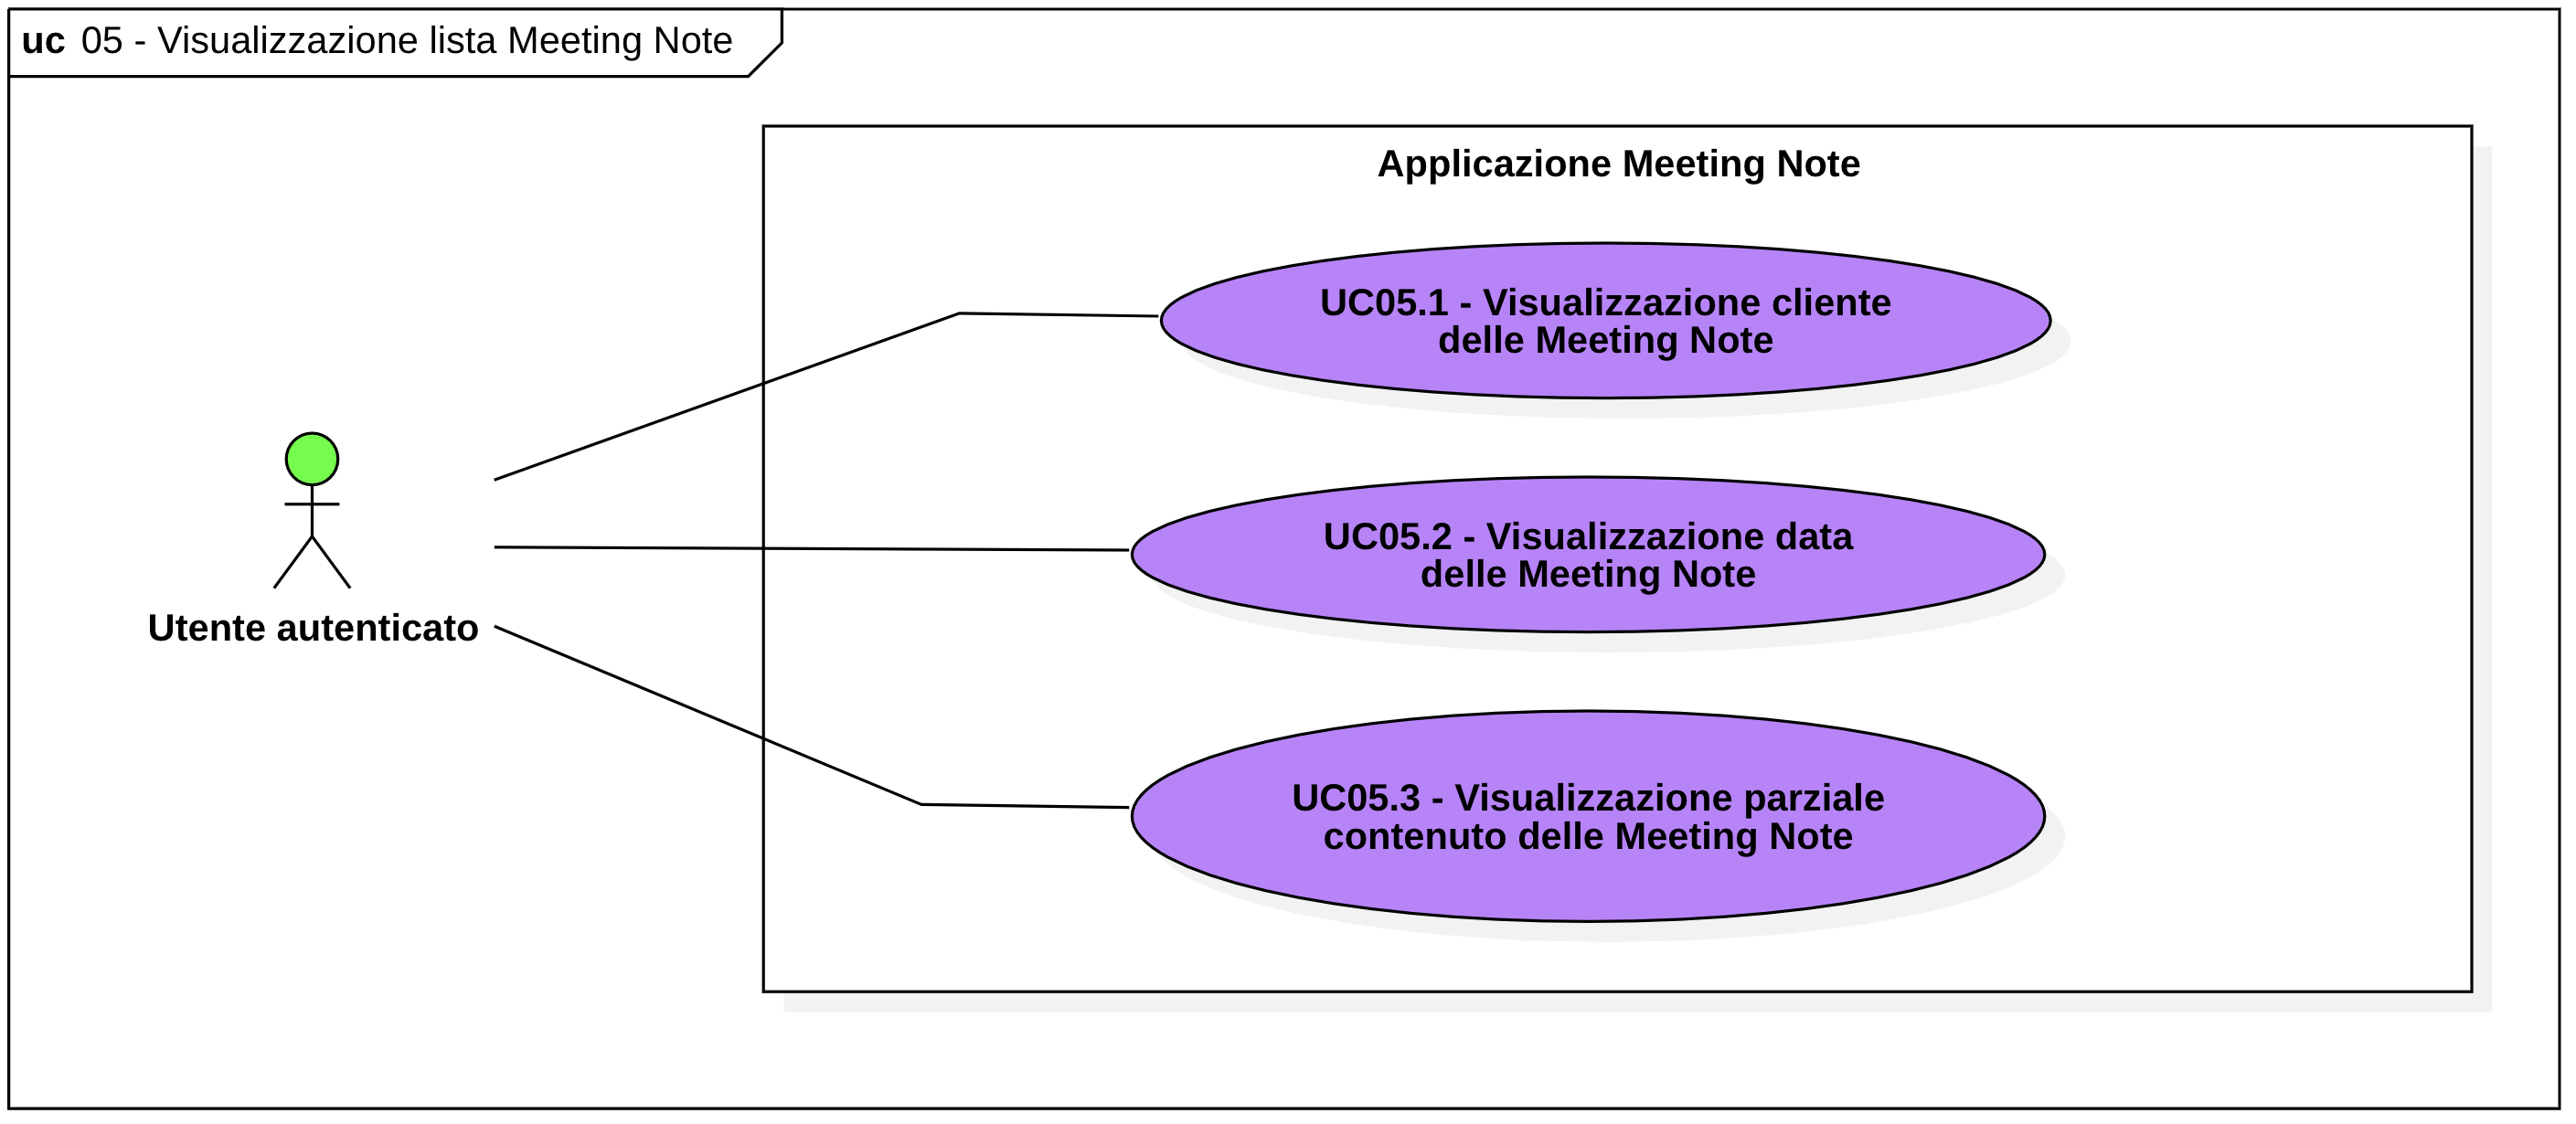
\includegraphics[width=1.0\columnwidth]{usecase/3-uc} 
    \caption{Use Case - Visualizzazione lista Meeting Note}
    \label{fig:uc-meetingnote-list-details}
\end{figure}

\begin{usecase}{05.1}{Visualizzazione cliente delle Meeting Note}
    \usecasemainactors{Utente autenticato}
    \usecasepre{L'utente visualizza la lista delle \gls{meetingnote}\glsoccur}
    \usecasedesc{L'utente vuole visualizzare gli identificativi dei \glspl{cliente}\glsoccur associati alle \gls{meetingnote}\glsoccur.}
    \usecasepost{Sono visualizzabili i \glspl{cliente}\glsoccur associati alle \gls{meetingnote}\glsoccur}
    \usecaseimg{\ref{fig:uc-meetingnote-list-details}}
    \label{UC05.1}
\end{usecase}

\begin{usecase}{05.2}{Visualizzazione data della Meeting Note}
    \usecasemainactors{Utente autenticato}
    \usecasepre{L'utente visualizza la lista delle \gls{meetingnote}\glsoccur}
    \usecasedesc{L'utente vuole visualizzare le date degli incontri associati alle \gls{meetingnote}\glsoccur.}
    \usecasepost{Sono visualizzabili le date degli incontri associati alle \gls{meetingnote}\glsoccur}
    \usecaseimg{\ref{fig:uc-meetingnote-list-details}}
    \label{UC05.2}
\end{usecase}

\begin{usecase}{05.3}{Visualizzazione parziale contenuto delle Meeting Note}
    \usecasemainactors{Utente autenticato}
    \usecasepre{L'utente visualizza la lista delle \gls{meetingnote}\glsoccur}
    \usecasedesc{L'utente vuole visualizzare parzialmente i contenuti delle \gls{meetingnote}\glsoccur.}
    \usecasepost{Sono visualizzabili parzialmente i contenuti delle \gls{meetingnote}\glsoccur}
    \usecaseimg{\ref{fig:uc-meetingnote-list-details}}
    \label{UC05.3}
\end{usecase}

\begin{usecase}{06}{Errore visualizzazione lista Meeting Note}
    \usecasemainactors{Utente autenticato}
    \usecasesecondaryactors{\emph{RiskAPP API}}
    \usecasepre{L'utente è autenticato nel sistema}
    \usecasedesc{La visualizzazione della lista delle \gls{meetingnote}\glsoccur fallisce e l'utente viene informato dell'errore; le motivazioni possono essere le seguenti:
        \begin{itemize}
            \item la lista è vuota;
            \item il sistema non è raggiungibile;
            \item token di autenticazione scaduto;
            \item connessione ad internet assente.
        \end{itemize}}
    \usecasepost{Non è visualizzabile la lista delle \gls{meetingnote}\glsoccur}
    \usecaseimg{\ref{fig:uc-meetingnote}}
    \label{UC06}
\end{usecase}

\begin{usecase}{07}{Ricerca Meeting Note}
    \usecasemainactors{Utente autenticato}
    \usecasepre{L'utente visualizza la lista delle \gls{meetingnote}\glsoccur a lui associate}
    \usecasedesc{L'utente effettua una ricerca all'interno della lista delle \gls{meetingnote}\glsoccur.}
    \usecasepost{Lista delle \gls{meetingnote}\glsoccur è filtrata}
    \usecaseimg{\ref{fig:uc-meetingnote}}
    \label{UC07}
\end{usecase}

\newpage

\begin{figure}[!h] 
    \centering 
    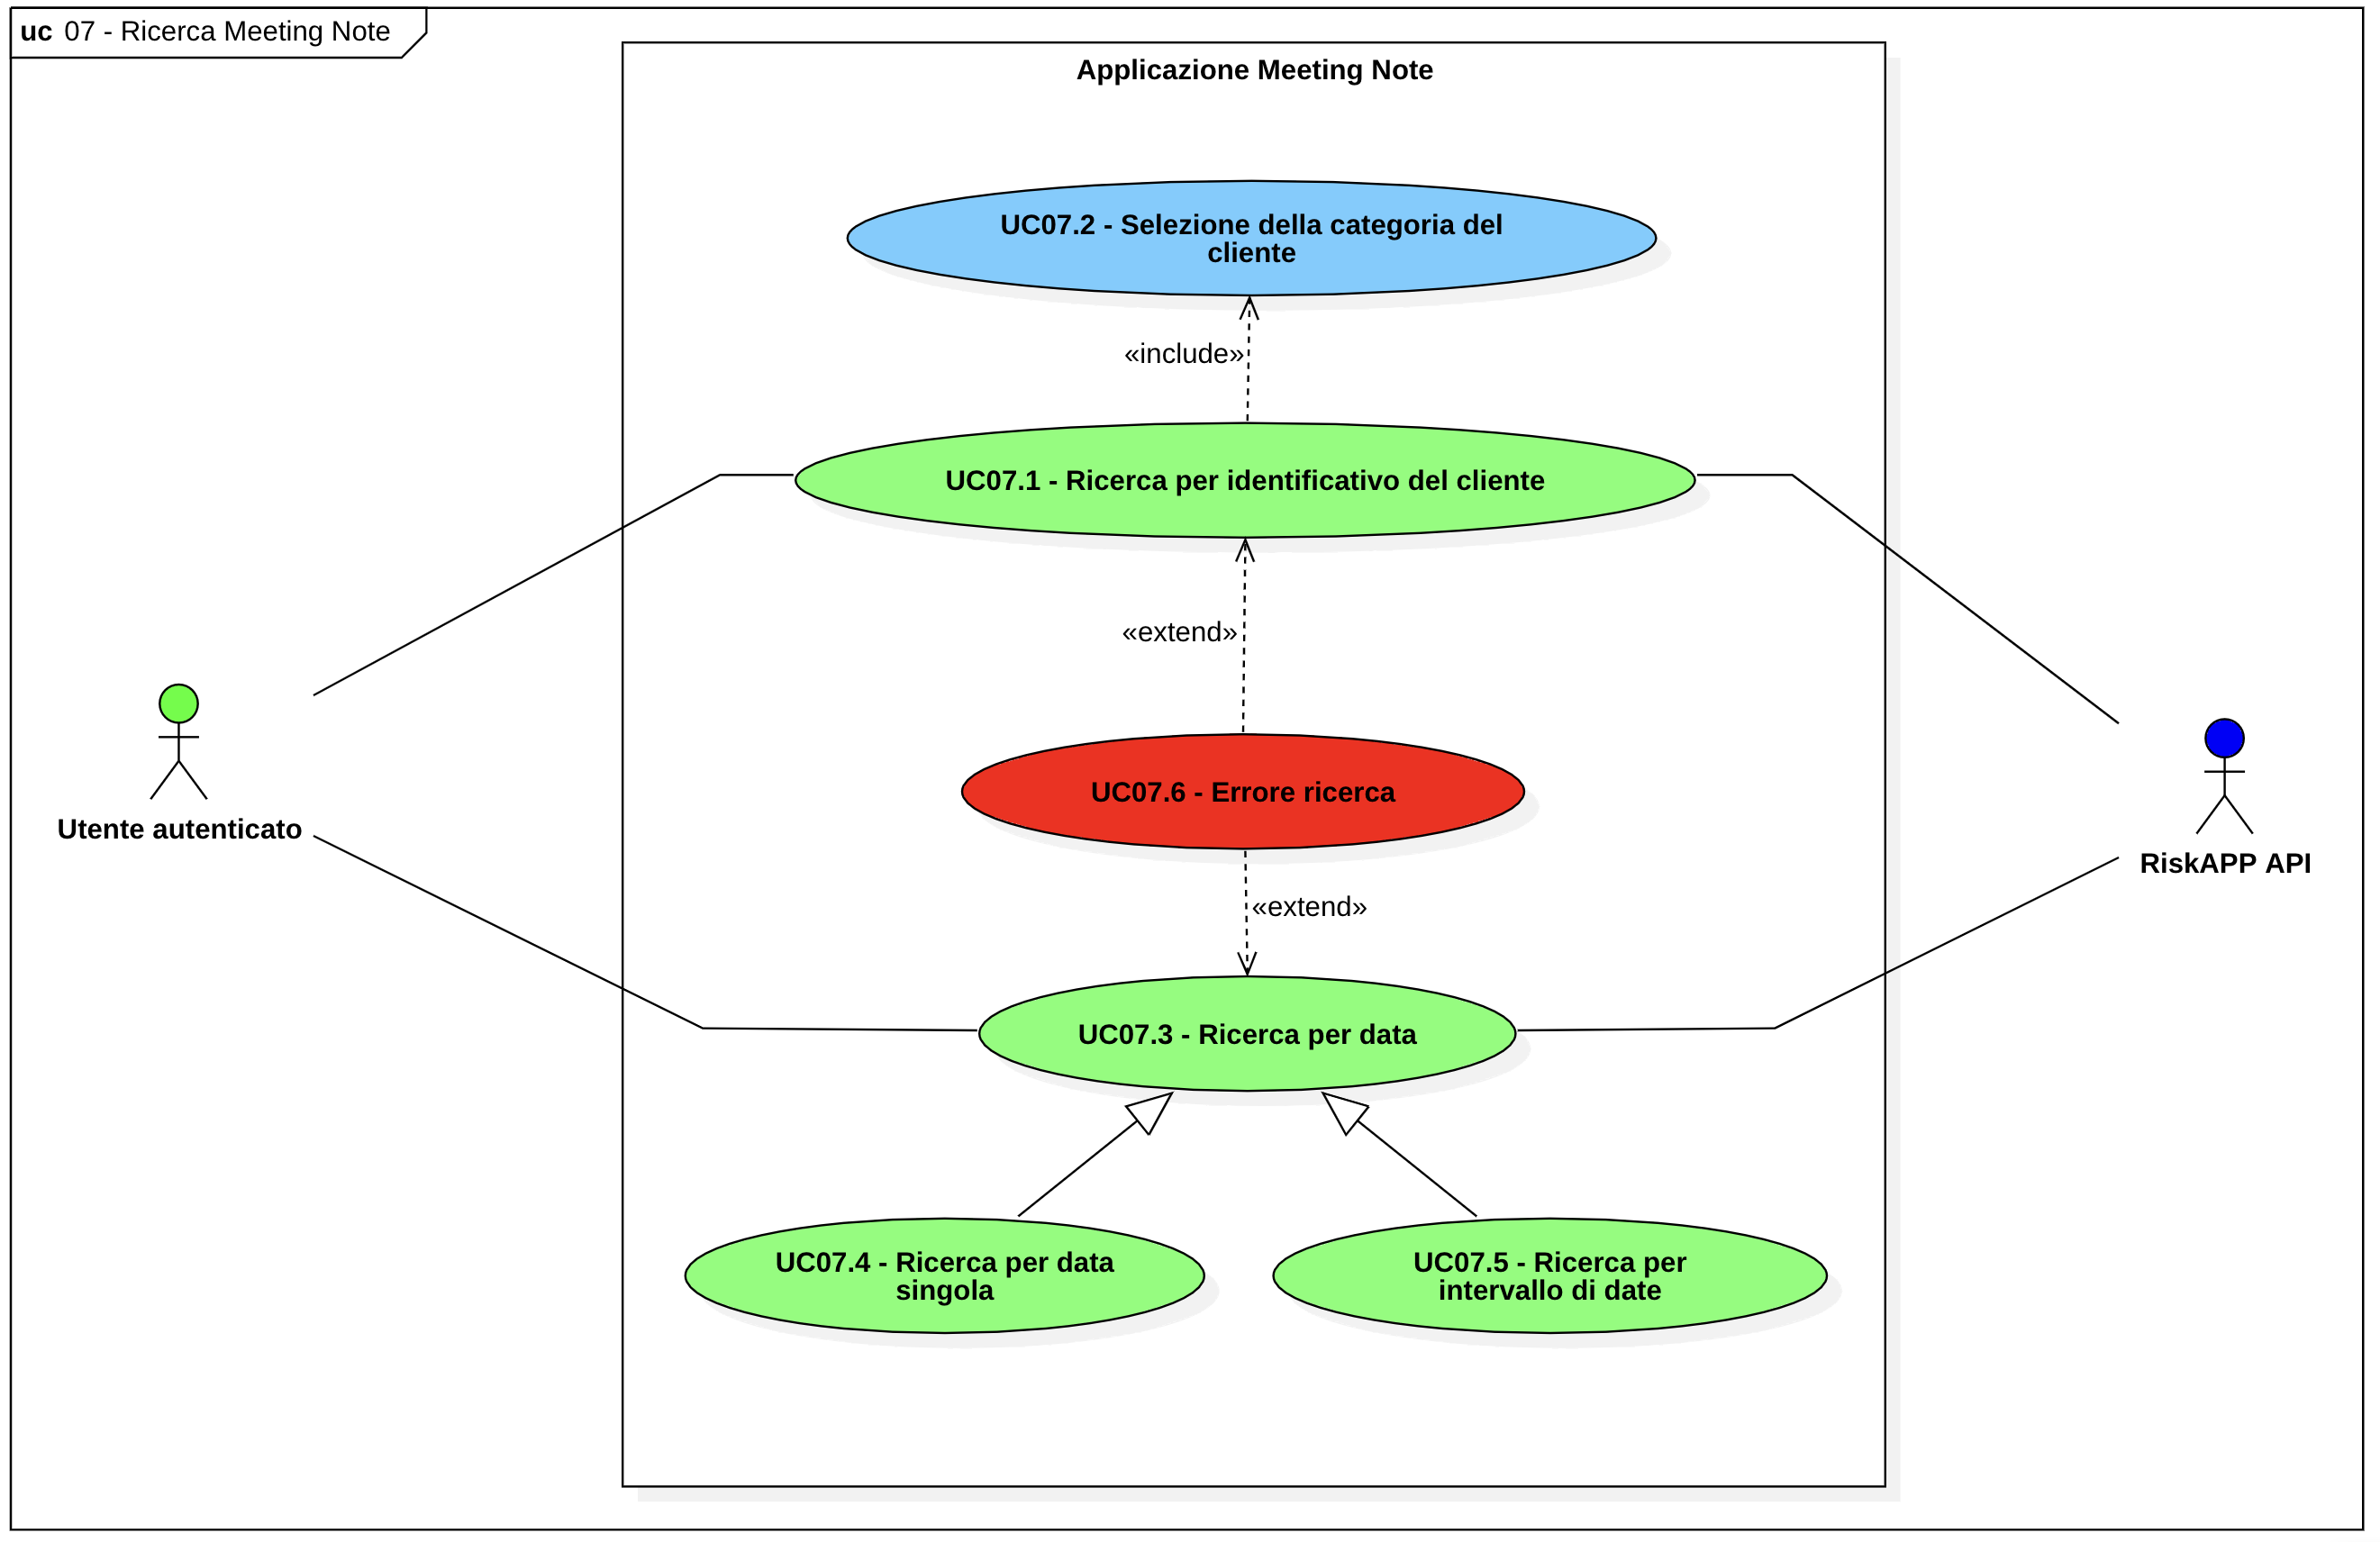
\includegraphics[width=1.0\columnwidth]{usecase/4-uc} 
    \caption{Use Case - Ricerca Meeting Note}
    \label{fig:uc-meetingnote-search}
\end{figure}

\begin{usecase}{07.1}{Ricerca per identificativo del cliente}
    \usecasemainactors{Utente autenticato}
    \usecasesecondaryactors{\emph{RiskAPP API}}
    \usecasepre{L'utente ha selezionato la categoria del \gls{cliente}\glsoccur}
    \usecasedesc{L'utente effettua una ricerca per identificativo del \gls{cliente}\glsoccur all'interno della lista delle \gls{meetingnote}\glsoccur.}
    \usecasepost{Lista delle \gls{meetingnote}\glsoccur è filtrata per identificativo del \gls{cliente}\glsoccur}
    \usecasealt{Se la ricerca fallisce, si verifica \hyperref[UC07.6]{UC07.6}}
    \usecaseimg{\ref{fig:uc-meetingnote-search}}
    \label{UC07.1}
\end{usecase}

\begin{usecase}{07.2}{Selezione della categoria del cliente}
    \usecasemainactors{Utente autenticato}
    \usecasepre{L'utente visualizza la lista delle \gls{meetingnote}\glsoccur a lui associate}
    \usecasedesc{L'utente seleziona la categoria del \gls{cliente}\glsoccur per effettuare la ricerca per identificativo all'interno della lista delle \gls{meetingnote}\glsoccur.}
    \usecasepost{La categoria del \gls{cliente}\glsoccur è selezionata}
    \usecaseimg{\ref{fig:uc-meetingnote-search}}
    \label{UC07.2}
\end{usecase}

\begin{usecase}{07.3}{Ricerca per data}
    \usecasemainactors{Utente autenticato}
    \usecasesecondaryactors{\emph{RiskAPP API}}
    \usecasepre{L'utente visualizza la lista delle \gls{meetingnote}\glsoccur a lui associate}
    \usecasedesc{L'utente effettua una ricerca per data all'interno della lista delle \gls{meetingnote}\glsoccur.}
    \usecasepost{Lista delle \gls{meetingnote}\glsoccur è filtrata per data}
    \usecasealt{Se la ricerca fallisce, si verifica \hyperref[UC07.6]{UC07.6}}
    \usecaseimg{\ref{fig:uc-meetingnote-search}}
    \label{UC07.3}
\end{usecase}

\begin{usecase}{07.4}{Ricerca per data singola}
    \usecasemainactors{Utente autenticato}
    \usecasepre{L'utente visualizza la lista delle \gls{meetingnote}\glsoccur a lui associate}
    \usecasedesc{L'utente effettua una ricerca per data singola all'interno della lista delle \gls{meetingnote}\glsoccur.}
    \usecasepost{Lista delle \gls{meetingnote}\glsoccur è filtrata per data singola}
    \usecaseimg{\ref{fig:uc-meetingnote-search}}
    \label{UC07.4}
\end{usecase}

\begin{usecase}{07.5}{Ricerca per intervallo di date}
    \usecasemainactors{Utente autenticato}
    \usecasepre{L'utente visualizza la lista delle \gls{meetingnote}\glsoccur a lui associate}
    \usecasedesc{L'utente effettua una ricerca per intervallo di date all'interno della lista delle \gls{meetingnote}\glsoccur.}
    \usecasepost{Lista delle \gls{meetingnote}\glsoccur è filtrata per intervallo di date}
    \usecaseimg{\ref{fig:uc-meetingnote-search}}
    \label{UC07.5}
\end{usecase}

\begin{usecase}{07.6}{Errore ricerca}
    \usecasemainactors{Utente autenticato}
    \usecasesecondaryactors{\emph{RiskAPP API}}
    \usecasepre{L'utente ha effettuato una ricerca all'interno della lista delle \gls{meetingnote}\glsoccur}
    \usecasedesc{La ricerca fallisce e l'utente viene informato dell'errore; le motivazioni possono essere le seguenti:
        \begin{itemize}
            \item la lista risultante è vuota;
            \item il sistema non è raggiungibile;
            \item token di autenticazione scaduto;
            \item connessione ad internet assente.
        \end{itemize}}
    \usecasepost{Lista delle \gls{meetingnote}\glsoccur non è filtrata}
    \usecaseimg{\ref{fig:uc-meetingnote-search}}
    \label{UC07.6}
\end{usecase}

\begin{usecase}{08}{Visualizzazione dati utente}
    \usecasemainactors{Utente autenticato}
    \usecasesecondaryactors{\emph{RiskAPP API}}
    \usecasepre{L'utente è autenticato nel sistema}
    \usecasedesc{L'utente vuole visualizzare i propri dati personali.}
    \usecasepost{Sono visualizzabili i dati personali dell'utente}
    \usecasealt{Se la visualizzazione fallisce, si verifica \hyperref[UC09]{UC09}} 
    \usecaseimg{\ref{fig:uc-meetingnote}}
    \label{UC08}
\end{usecase}

\begin{figure}[!h] 
    \centering 
    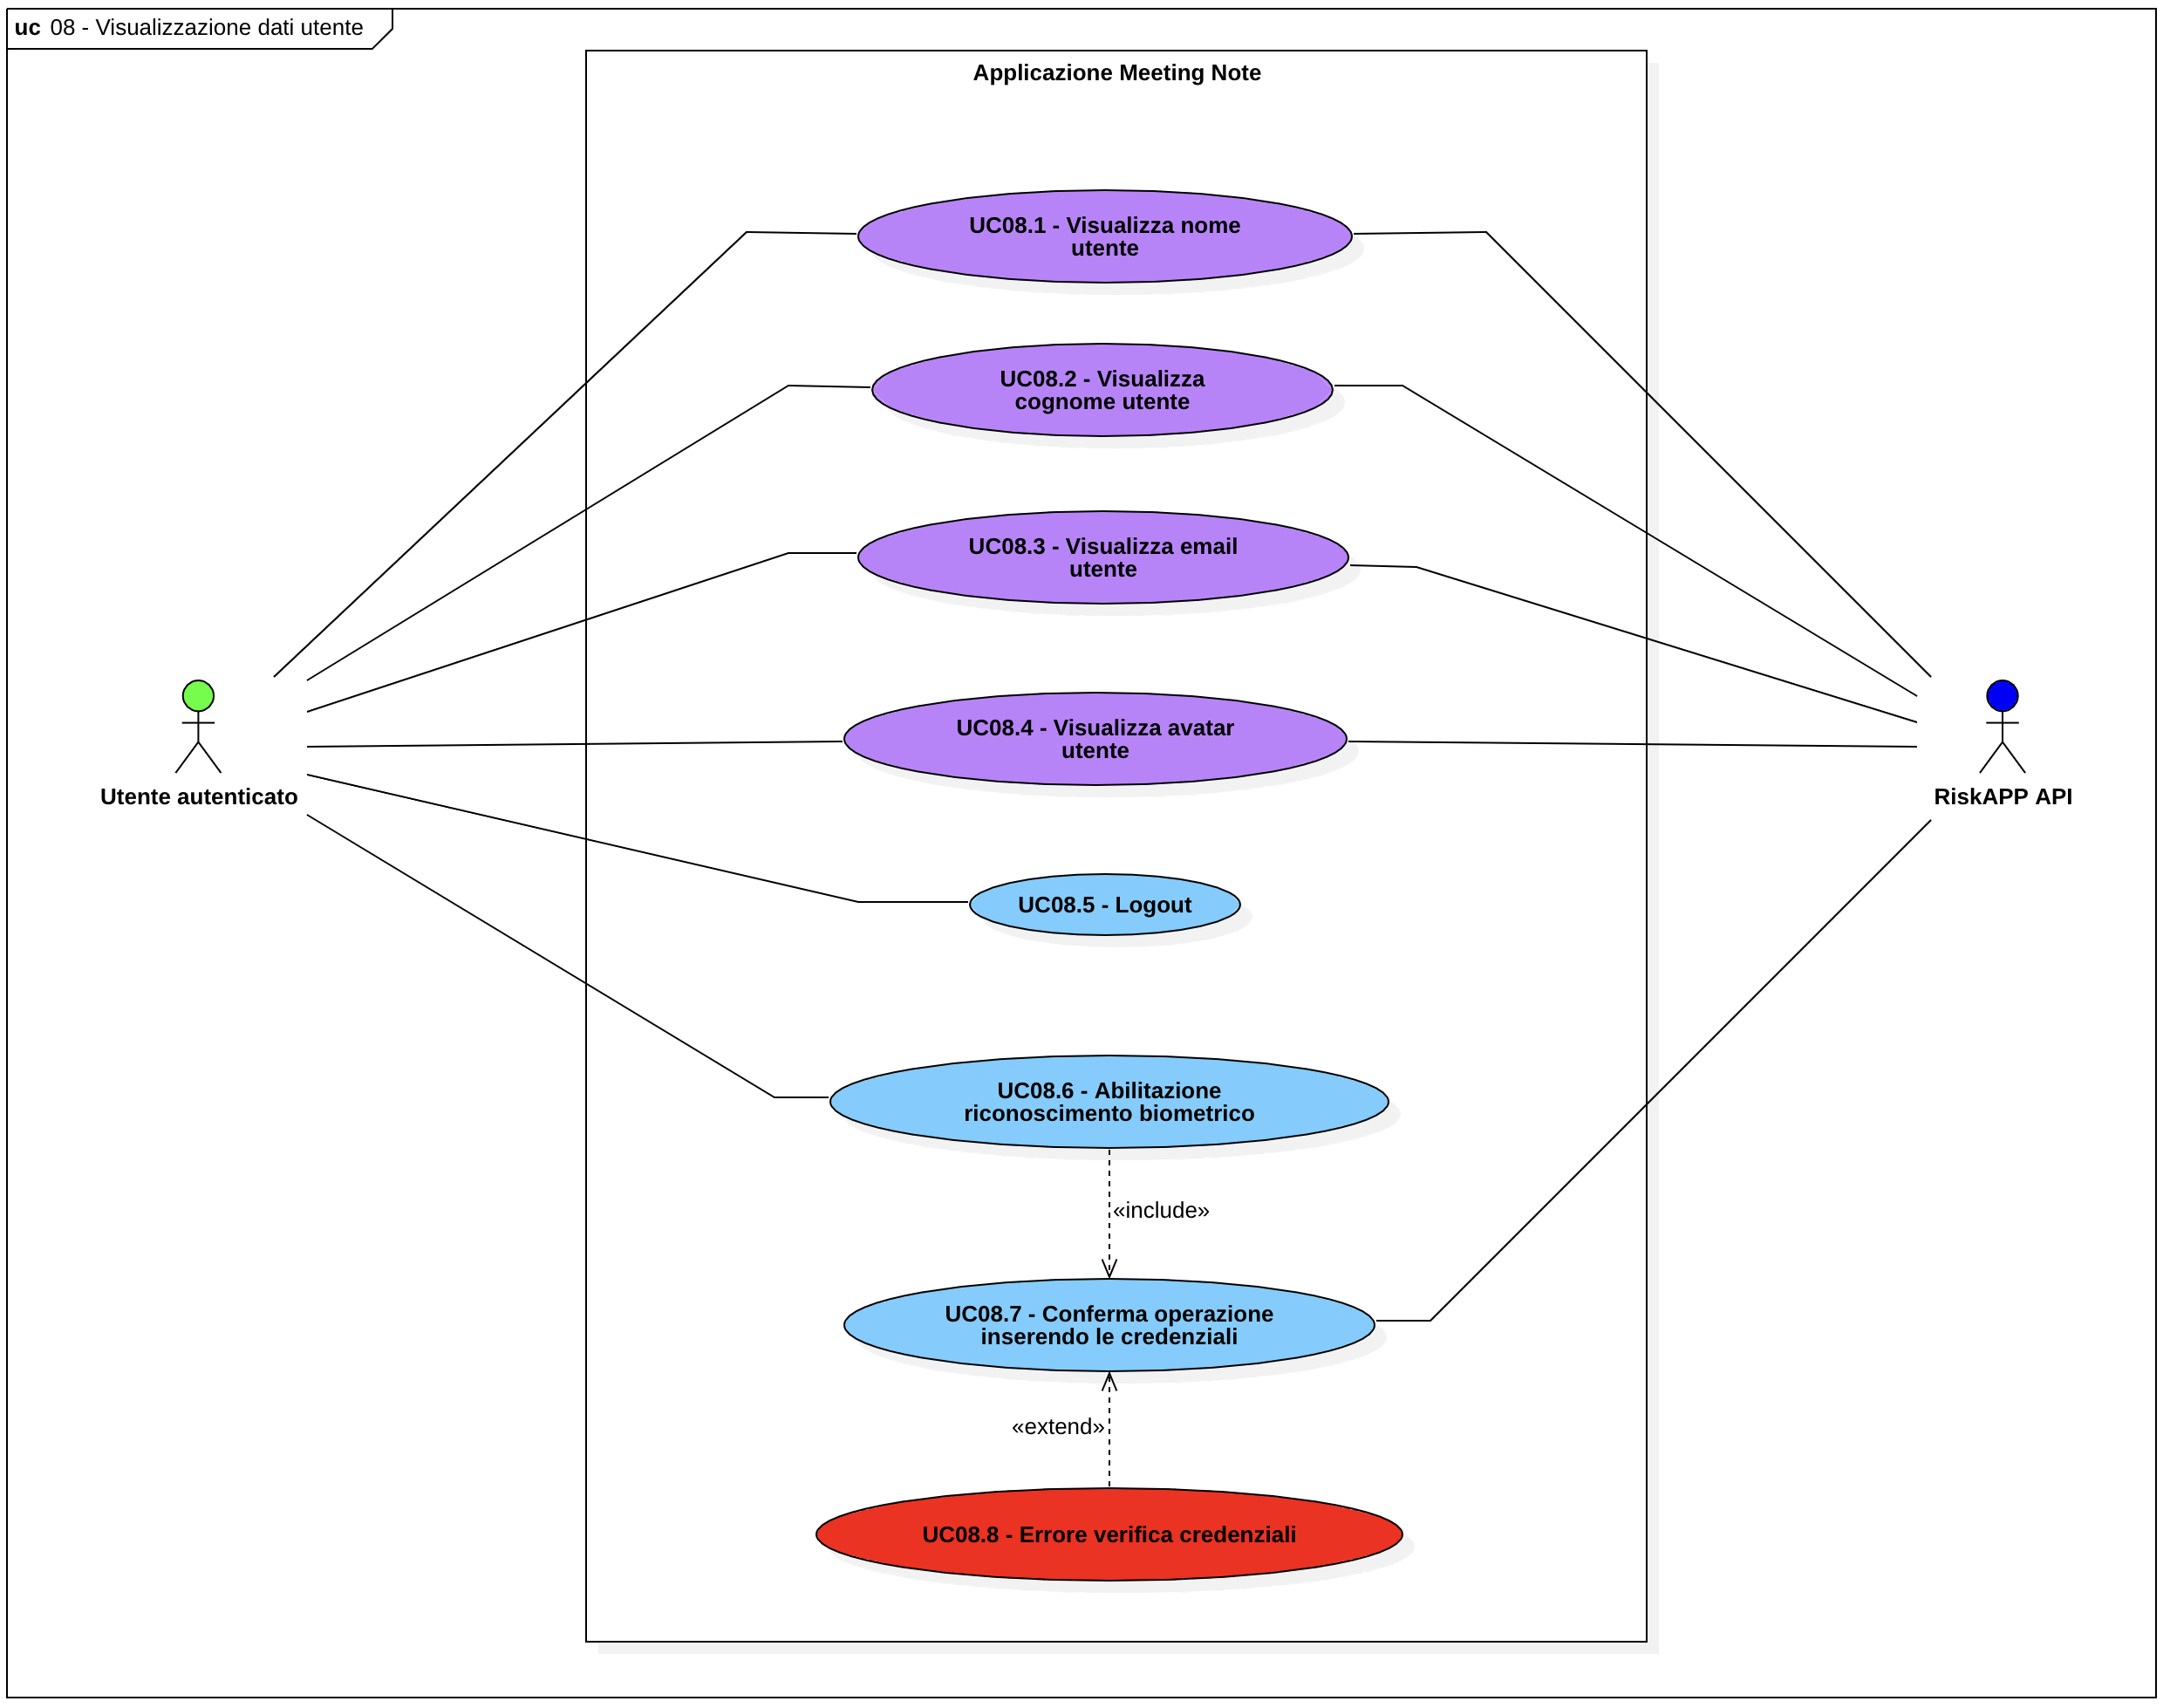
\includegraphics[width=1.0\columnwidth]{usecase/5-uc} 
    \caption{Use Case - Visualizzazione dati utente}
    \label{fig:uc-user}
\end{figure}

\begin{usecase}{08.1}{Visualizzazione nome utente}
    \usecasemainactors{Utente autenticato}
    \usecasesecondaryactors{\emph{RiskAPP API}}
    \usecasepre{L'utente visualizza i propri dati personali}
    \usecasedesc{L'utente vuole visualizzare il proprio nome.}
    \usecasepost{È visualizzabile il nome dell'utente}
    \usecaseimg{\ref{fig:uc-user}}
    \label{UC08.1}
\end{usecase}

\begin{usecase}{08.2}{Visualizzazione cognome utente}
    \usecasemainactors{Utente autenticato}
    \usecasesecondaryactors{\emph{RiskAPP API}}
    \usecasepre{L'utente visualizza i propri dati personali}
    \usecasedesc{L'utente vuole visualizzare il proprio cognome.}
    \usecasepost{È visualizzabile il cognome dell'utente}
    \usecaseimg{\ref{fig:uc-user}}
    \label{UC08.2}
\end{usecase}

\begin{usecase}{08.3}{Visualizzazione email utente}
    \usecasemainactors{Utente autenticato}
    \usecasesecondaryactors{\emph{RiskAPP API}}
    \usecasepre{L'utente visualizza i propri dati personali}
    \usecasedesc{L'utente vuole visualizzare la propria email.}
    \usecasepost{È visualizzabile la email dell'utente}
    \usecaseimg{\ref{fig:uc-user}}
    \label{UC08.3}
\end{usecase}

\begin{usecase}{08.4}{Visualizzazione avatar utente}
    \usecasemainactors{Utente autenticato}
    \usecasesecondaryactors{\emph{RiskAPP API}}
    \usecasepre{L'utente visualizza i propri dati personali}
    \usecasedesc{L'utente vuole visualizzare il proprio avatar.}
    \usecasepost{È visualizzabile l'avatar dell'utente}
    \usecaseimg{\ref{fig:uc-user}}
    \label{UC08.4}
\end{usecase}

\begin{usecase}{08.5}{Logout}
    \usecasemainactors{Utente autenticato}
    \usecasepre{L'utente visualizza i propri dati personali}
    \usecasedesc{L'utente vuole effetuare il logout.}
    \usecasepost{L'utente non è più autenticato al sistema}
    \usecaseimg{\ref{fig:uc-user}}
    \label{UC08.5}
\end{usecase}

\begin{usecase}{08.6}{Abilitazione riconoscimento biometrico}
    \usecasemainactors{Utente autenticato}
    \usecasesecondaryactors{\emph{RiskAPP API}}
    \usecasepre{L'utente visualizza i propri dati personali}
    \usecasedesc{L'utente vuole abilitare il \gls{riconoscimentobiometrico}\glsoccur, deve inserire le proprie credenziali per la conferma.}
    \usecasepost{Riconoscimento biometrico abilitato}
    \usecaseimg{\ref{fig:uc-user}}
    \label{UC08.6}
\end{usecase}

\begin{usecase}{08.7}{Conferma operazione inserendo le credenziali}
    \usecasemainactors{Utente autenticato}
    \usecasesecondaryactors{\emph{RiskAPP API}}
    \usecasepre{L'utente visualizza i propri dati personali}
    \usecasedesc{L'utente inserisce le proprie credenziali per abilitare il \gls{riconoscimentobiometrico}\glsoccur.}
    \usecasepost{Riconoscimento biometrico abilitato}
    \usecasealt{Se la conferma fallisce, si verifica \hyperref[UC08.8]{UC08.8}}
    \usecaseimg{\ref{fig:uc-user}}
    \label{UC08.7}
\end{usecase}

\begin{usecase}{08.8}{Errore verifica credenziali}
    \usecasemainactors{Utente autenticato}
    \usecasesecondaryactors{\emph{RiskAPP API}}
    \usecasepre{L'utente visualizza i propri dati personali}
    \usecasedesc{La verifica delle credenziali fallisce e l'utente viene informato dell'errore; le motivazioni possono essere le seguenti:
        \begin{itemize}
            \item le credenziali inserite non sono corrette;
            \item il sistema non è raggiungibile;
            \item connessione ad internet assente.
        \end{itemize}}
    \usecasepost{Riconoscimento biometrico non abilitato}
    \usecaseimg{\ref{fig:uc-user}}
    \label{UC08.8}
\end{usecase}

\begin{usecase}{09}{Errore visualizzazione dati utente}
    \usecasemainactors{Utente autenticato}
    \usecasesecondaryactors{\emph{RiskAPP API}}
    \usecasepre{L'utente è autenticato nel sistema}
    \usecasedesc{La visualizzazione dei dati utente fallisce e l'utente viene informato dell'errore; le motivazioni possono essere le seguenti:
        \begin{itemize}
            \item il sistema non è raggiungibile;
            \item token di autenticazione scaduto;
            \item connessione ad internet assente.
        \end{itemize}}
    \usecasepost{Non sono visualizzabili i dati personali dell'utente}
    \usecaseimg{\ref{fig:uc-meetingnote}}
    \label{UC09}
\end{usecase}

\begin{usecase}{10}{Ordinamento lista Meeting Note}
    \usecasemainactors{Utente autenticato}
    \usecasesecondaryactors{\emph{RiskAPP API}}
    \usecasepre{L'utente visualizza la lista delle \gls{meetingnote}\glsoccur}
    \usecasedesc{L'utente vuole ordinare la lista delle \gls{meetingnote}\glsoccur.}
    \usecasepost{Lista delle \gls{meetingnote}\glsoccur è ordinata}
    \usecasealt{Se l'ordinamento fallisce, si verifica \hyperref[UC13]{UC13}}
    \usecaseimg{\ref{fig:uc-meetingnote}}
    \label{UC10}
\end{usecase}

\begin{usecase}{11}{Ordinamento dalla meno recente}
    \usecasemainactors{Utente autenticato}
    \usecasesecondaryactors{\emph{RiskAPP API}}
    \usecasepre{L'utente visualizza la lista delle \gls{meetingnote}\glsoccur}
    \usecasedesc{L'utente vuole ordinare la lista delle \gls{meetingnote}\glsoccur dalla meno recente.}
    \usecasepost{Lista delle \gls{meetingnote}\glsoccur è ordinata dalla meno recente}
    \usecasealt{Se l'ordinamento fallisce, si verifica \hyperref[UC13]{UC13}}
    \usecaseimg{\ref{fig:uc-meetingnote}}
    \label{UC11}
\end{usecase}

\begin{usecase}{12}{Ordinamento dalla più recente}
    \usecasemainactors{Utente autenticato}
    \usecasesecondaryactors{\emph{RiskAPP API}}
    \usecasepre{L'utente visualizza la lista delle \gls{meetingnote}\glsoccur}
    \usecasedesc{L'utente vuole ordinare la lista delle \gls{meetingnote}\glsoccur dalla più recente.}
    \usecasepost{Lista delle \gls{meetingnote}\glsoccur è ordinata dalla più recente}
    \usecasealt{Se l'ordinamento fallisce, si verifica \hyperref[UC13]{UC13}}
    \usecaseimg{\ref{fig:uc-meetingnote}}
    \label{UC12}
\end{usecase}

\begin{usecase}{13}{Errore nell'ordinamento}
    \usecasemainactors{Utente autenticato}
    \usecasesecondaryactors{\emph{RiskAPP API}}
    \usecasepre{L'utente vuole ordinare la lista delle \gls{meetingnote}\glsoccur}
    \usecasedesc{L'ordinamento della lista delle \gls{meetingnote}\glsoccur fallisce e l'utente viene informato dell'errore; le motivazioni possono essere le seguenti:
        \begin{itemize}
            \item il sistema non è raggiungibile;
            \item token di autenticazione scaduto;
            \item connessione ad internet assente.
        \end{itemize}}
    \usecasepost{Lista delle \gls{meetingnote}\glsoccur non è ordinata}
    \usecaseimg{\ref{fig:uc-meetingnote}}
    \label{UC13}
\end{usecase}

\begin{usecase}{14}{Visualizzazione singola Meeting Note}
    \usecasemainactors{Utente autenticato}
    \usecasepre{L'utente visualizza la lista delle \gls{meetingnote}\glsoccur}
    \usecasedesc{L'utente vuole visualizzare i dettagli di una singola \gls{meetingnote}\glsoccur.}
    \usecasepost{Sono visualizzabili i dettagli di una singola \gls{meetingnote}\glsoccur}
    \usecaseimg{\ref{fig:uc-meetingnote}}
    \label{UC14}
\end{usecase}

\newpage

\begin{figure}[!h] 
    \centering 
    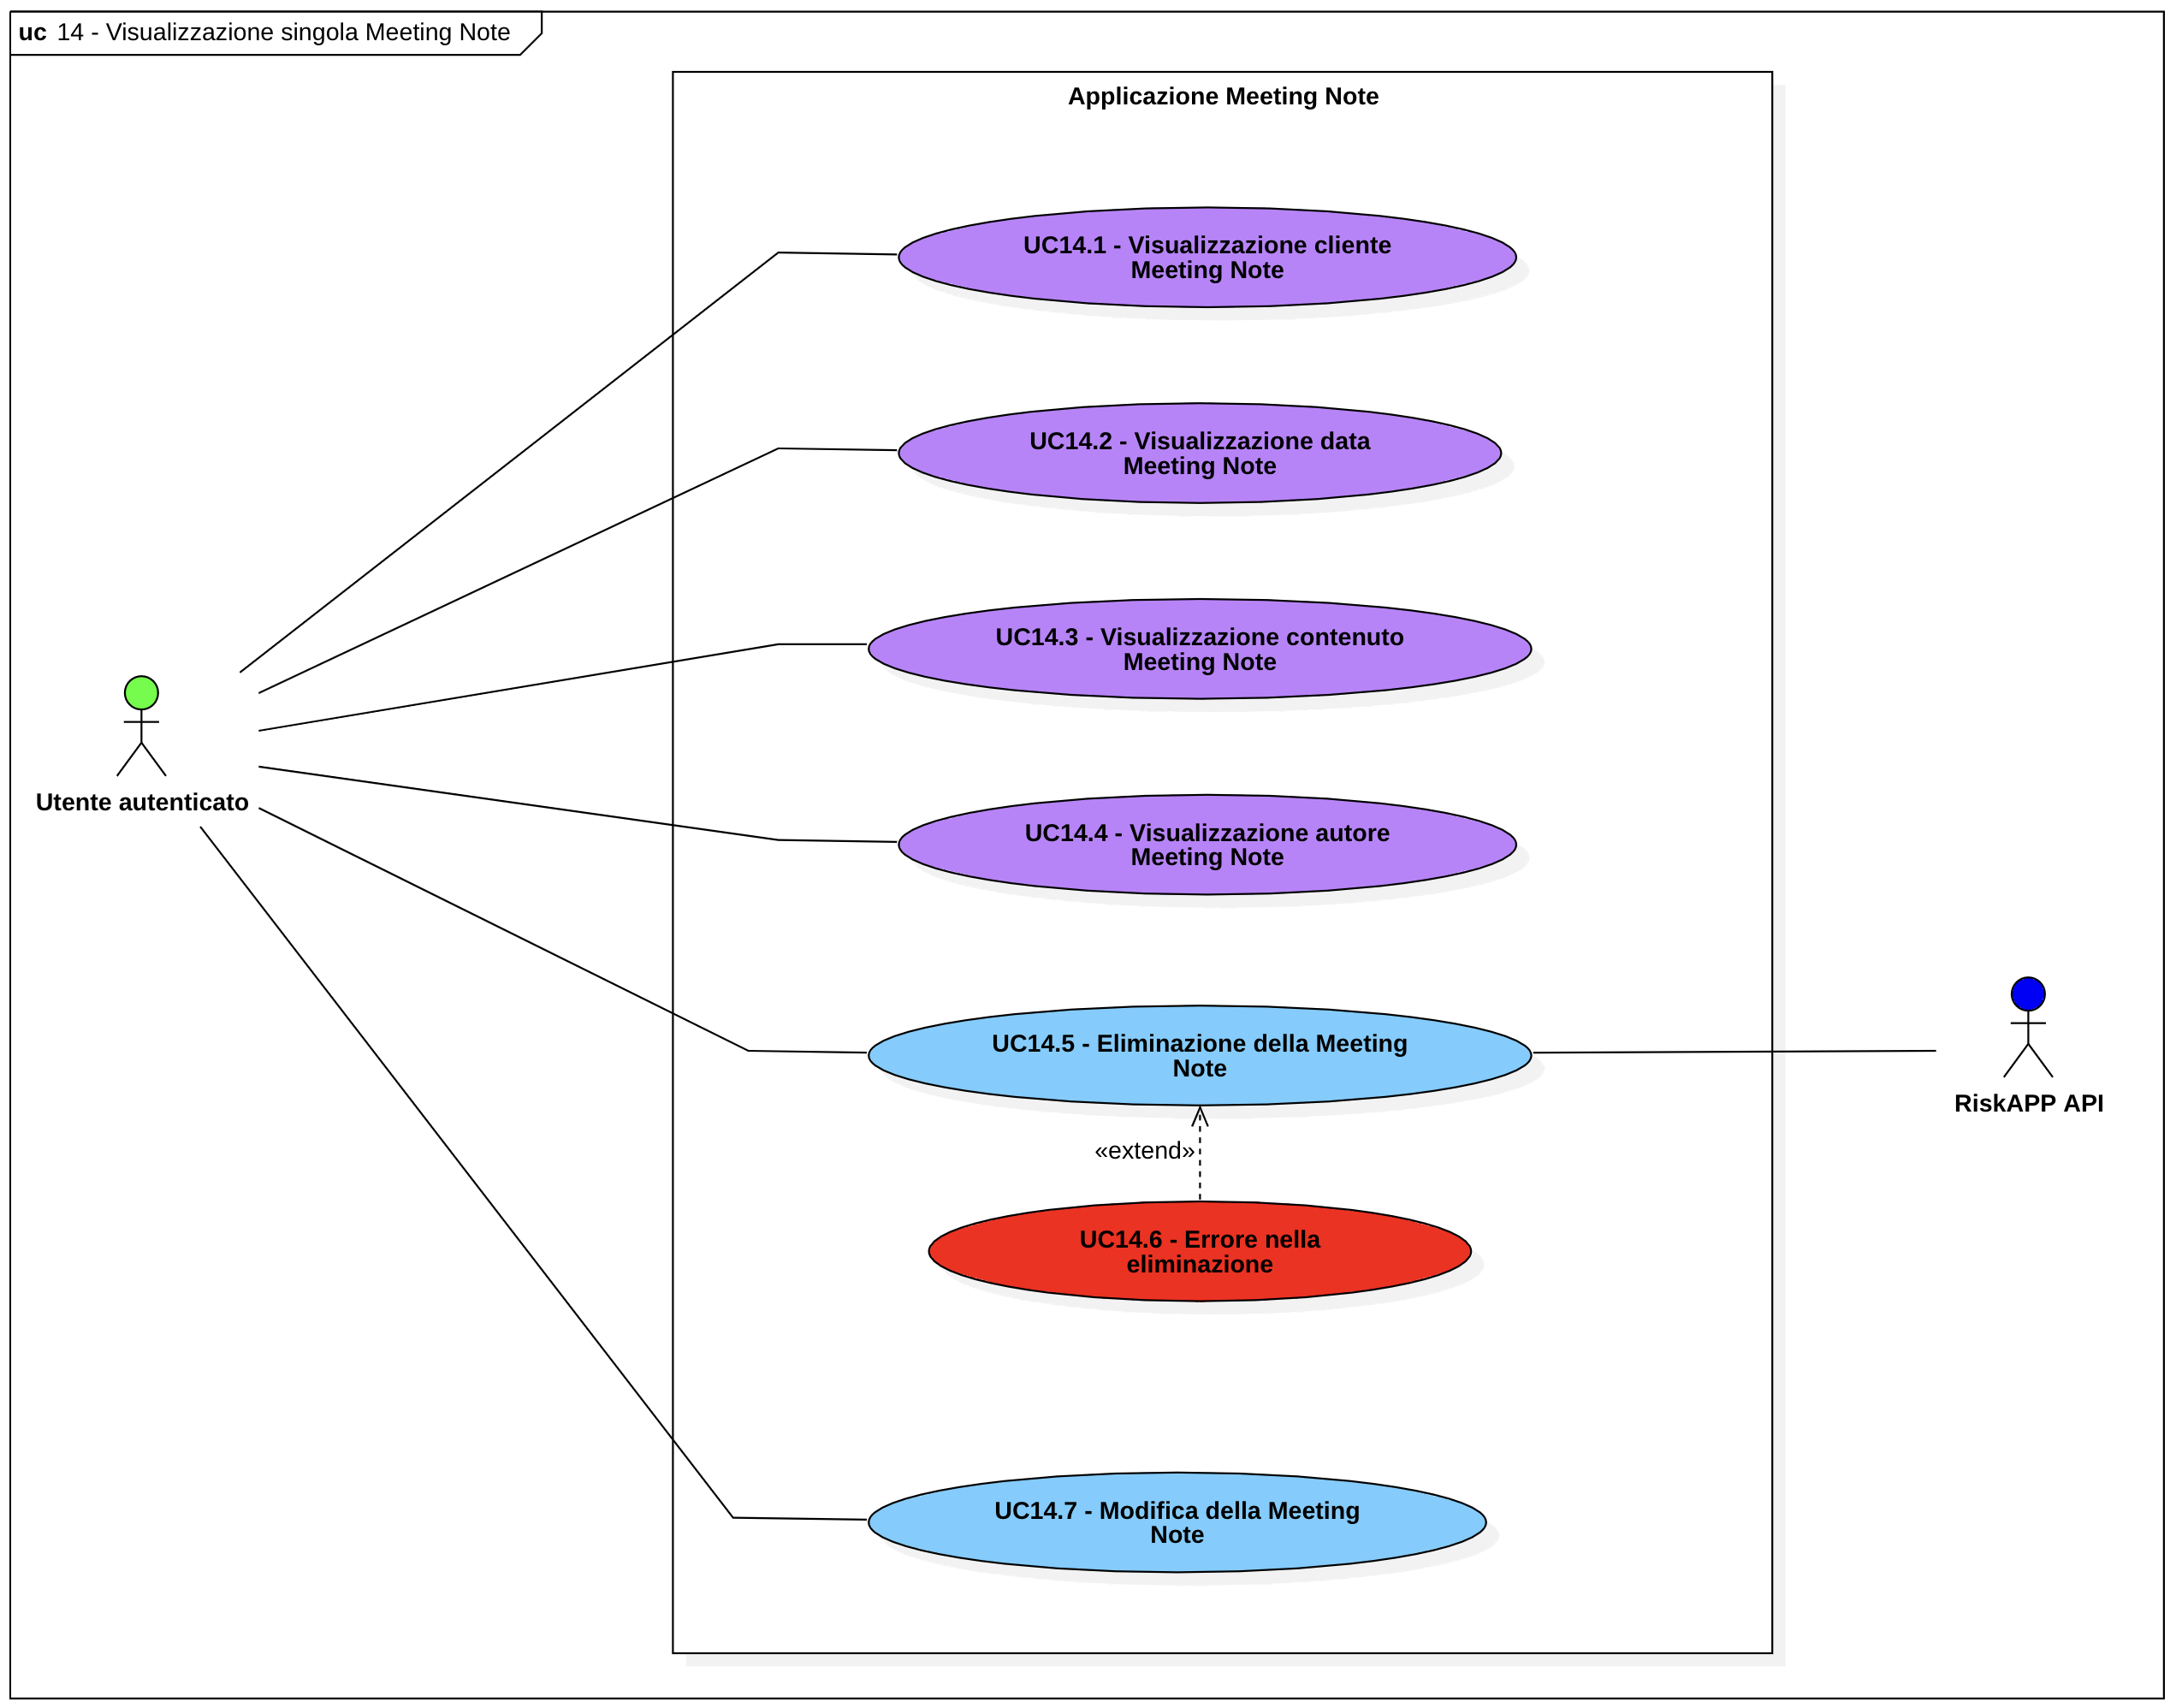
\includegraphics[width=1.0\columnwidth]{usecase/6-uc} 
    \caption{Use Case - Visualizzazione singola Meeting Note}
    \label{fig:uc-meetingnote-details}
\end{figure}

\begin{usecase}{14.1}{Visualizzazione cliente Meeting Note}
    \usecasemainactors{Utente autenticato}
    \usecasepre{L'utente visualizza i dettagli di una singola \gls{meetingnote}\glsoccur}
    \usecasedesc{L'utente vuole visualizzare il \gls{cliente}\glsoccur di una \gls{meetingnote}\glsoccur.}
    \usecasepost{È visualizzabile il \gls{cliente}\glsoccur di una \gls{meetingnote}\glsoccur}
    \usecaseimg{\ref{fig:uc-meetingnote-details}}
    \label{UC14.1}
\end{usecase}

\begin{usecase}{14.2}{Visualizzazione data Meeting Note}
    \usecasemainactors{Utente autenticato}
    \usecasepre{L'utente visualizza i dettagli di una singola \gls{meetingnote}\glsoccur}
    \usecasedesc{L'utente vuole visualizzare la data di una \gls{meetingnote}\glsoccur.}
    \usecasepost{È visualizzabile la data di una \gls{meetingnote}\glsoccur}
    \usecaseimg{\ref{fig:uc-meetingnote-details}}
    \label{UC14.2}
\end{usecase}

\begin{usecase}{14.3}{Visualizzazione contenuto Meeting Note}
    \usecasemainactors{Utente autenticato}
    \usecasepre{L'utente visualizza i dettagli di una singola \gls{meetingnote}\glsoccur}
    \usecasedesc{L'utente vuole visualizzare il contenuto di una \gls{meetingnote}\glsoccur.}
    \usecasepost{È visualizzabile il contenuto di una \gls{meetingnote}\glsoccur}
    \usecaseimg{\ref{fig:uc-meetingnote-details}}
    \label{UC14.3}
\end{usecase}

\begin{usecase}{14.4}{Visualizzazione autore Meeting Note}
    \usecasemainactors{Utente autenticato}
    \usecasepre{L'utente visualizza i dettagli di una singola \gls{meetingnote}\glsoccur}
    \usecasedesc{L'utente vuole visualizzare l'autore di una \gls{meetingnote}\glsoccur.}
    \usecasepost{È visualizzabile l'autore di una \gls{meetingnote}\glsoccur}
    \usecaseimg{\ref{fig:uc-meetingnote-details}}
    \label{UC14.4}
\end{usecase}

\begin{usecase}{14.5}{Eliminazione della Meeting Note}
    \usecasemainactors{Utente autenticato}
    \usecasesecondaryactors{\emph{RiskAPP API}}
    \usecasepre{L'utente visualizza i dettagli di una singola \gls{meetingnote}\glsoccur}
    \usecasedesc{L'utente vuole eliminare la \gls{meetingnote}\glsoccur selezionata.}
    \usecasepost{La \gls{meetingnote}\glsoccur selezionata è stata eliminata}
    \usecasealt{Se l'eliminazione fallisce, si verifica \hyperref[UC14.6]{UC14.6}}
    \usecaseimg{\ref{fig:uc-meetingnote-details}}
    \label{UC14.5}
\end{usecase}

\begin{usecase}{14.6}{Errore nella eliminazione}
    \usecasemainactors{Utente autenticato}
    \usecasesecondaryactors{\emph{RiskAPP API}}
    \usecasepre{L'utente visualizza i dettagli di una singola \gls{meetingnote}\glsoccur}
    \usecasedesc{L'eliminazione della \gls{meetingnote}\glsoccur selezionata fallisce e l'utente viene informato dell'errore; le motivazioni possono essere le seguenti:
        \begin{itemize}
            \item il sistema non è raggiungibile;
            \item token di autenticazione scaduto;
            \item connessione ad internet assente.
        \end{itemize}}
    \usecasepost{La \gls{meetingnote}\glsoccur selezionata non è stata eliminata}
    \usecaseimg{\ref{fig:uc-meetingnote-details}}
    \label{UC14.6}
\end{usecase}

\begin{usecase}{14.7}{Modifica della Meeting Note}
    \usecasemainactors{Utente autenticato}
    \usecasepre{L'utente visualizza i dettagli di una singola \gls{meetingnote}\glsoccur}
    \usecasedesc{L'utente vuole modificare la \gls{meetingnote}\glsoccur selezionata.}
    \usecasepost{La \gls{meetingnote}\glsoccur selezionata è stata modificata}
    \usecaseimg{\ref{fig:uc-meetingnote-details}}
    \label{UC14.7}
\end{usecase}

\newpage

\begin{figure}[!h] 
    \centering 
    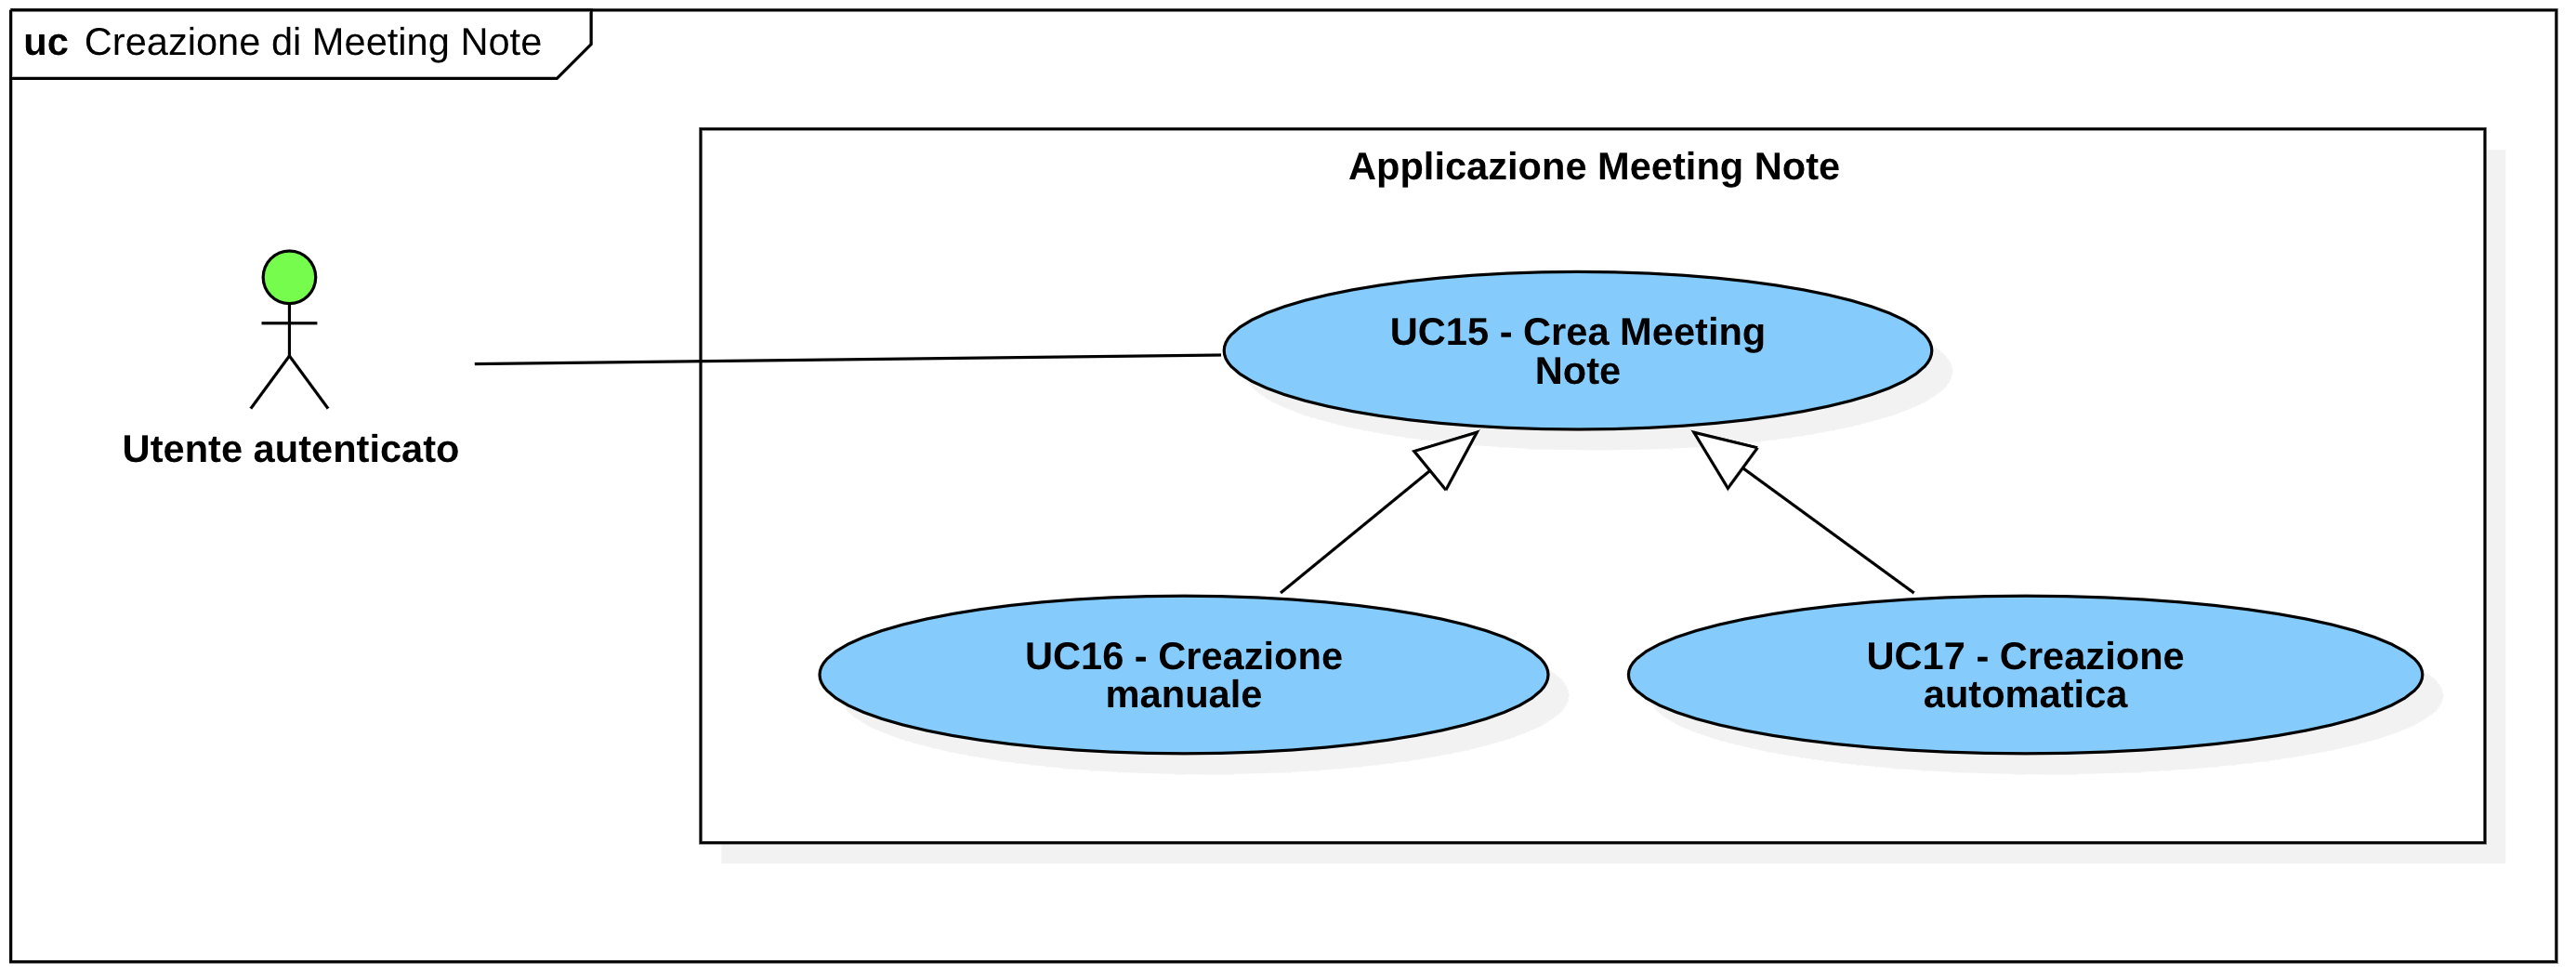
\includegraphics[width=1.0\columnwidth]{usecase/7-uc} 
    \caption{Use Case - Creazione Meeting Note}
    \label{fig:uc-meetingnote-create}
\end{figure}

\begin{usecase}{15}{Crea Meeting Note}
    \usecasemainactors{Utente autenticato}
    \usecasepre{L'utente è autenticato nel sistema}
    \usecasedesc{L'utente vuole creare una nuova \gls{meetingnote}\glsoccur.}
    \usecasepost{Una nuova \gls{meetingnote}\glsoccur è stata creata}
    \usecaseimg{\ref{fig:uc-meetingnote-create}}
    \label{UC15}
\end{usecase}

\begin{usecase}{16}{Creazione manuale}
    \usecasemainactors{Utente autenticato}
    \usecasepre{L'utente è autenticato nel sistema}
    \usecasedesc{L'utente vuole creare manualmente una nuova \gls{meetingnote}\glsoccur.}
    \usecasepost{Una nuova \gls{meetingnote}\glsoccur è stata creata manualmente}
    \usecaseimg{\ref{fig:uc-meetingnote-create}}
    \label{UC16}
\end{usecase}

\begin{usecase}{17}{Creazione automatica}
    \usecasemainactors{Utente autenticato}
    \usecasepre{L'utente è autenticato nel sistema}
    \usecasedesc{L'utente vuole creare automaticamente una nuova \gls{meetingnote}\glsoccur.}
    \usecasepost{Una nuova \gls{meetingnote}\glsoccur è stata creata automaticamente}
    \usecaseimg{\ref{fig:uc-meetingnote-create}}
    \label{UC17}
\end{usecase}

\newpage

\begin{figure}[!h] 
    \centering 
    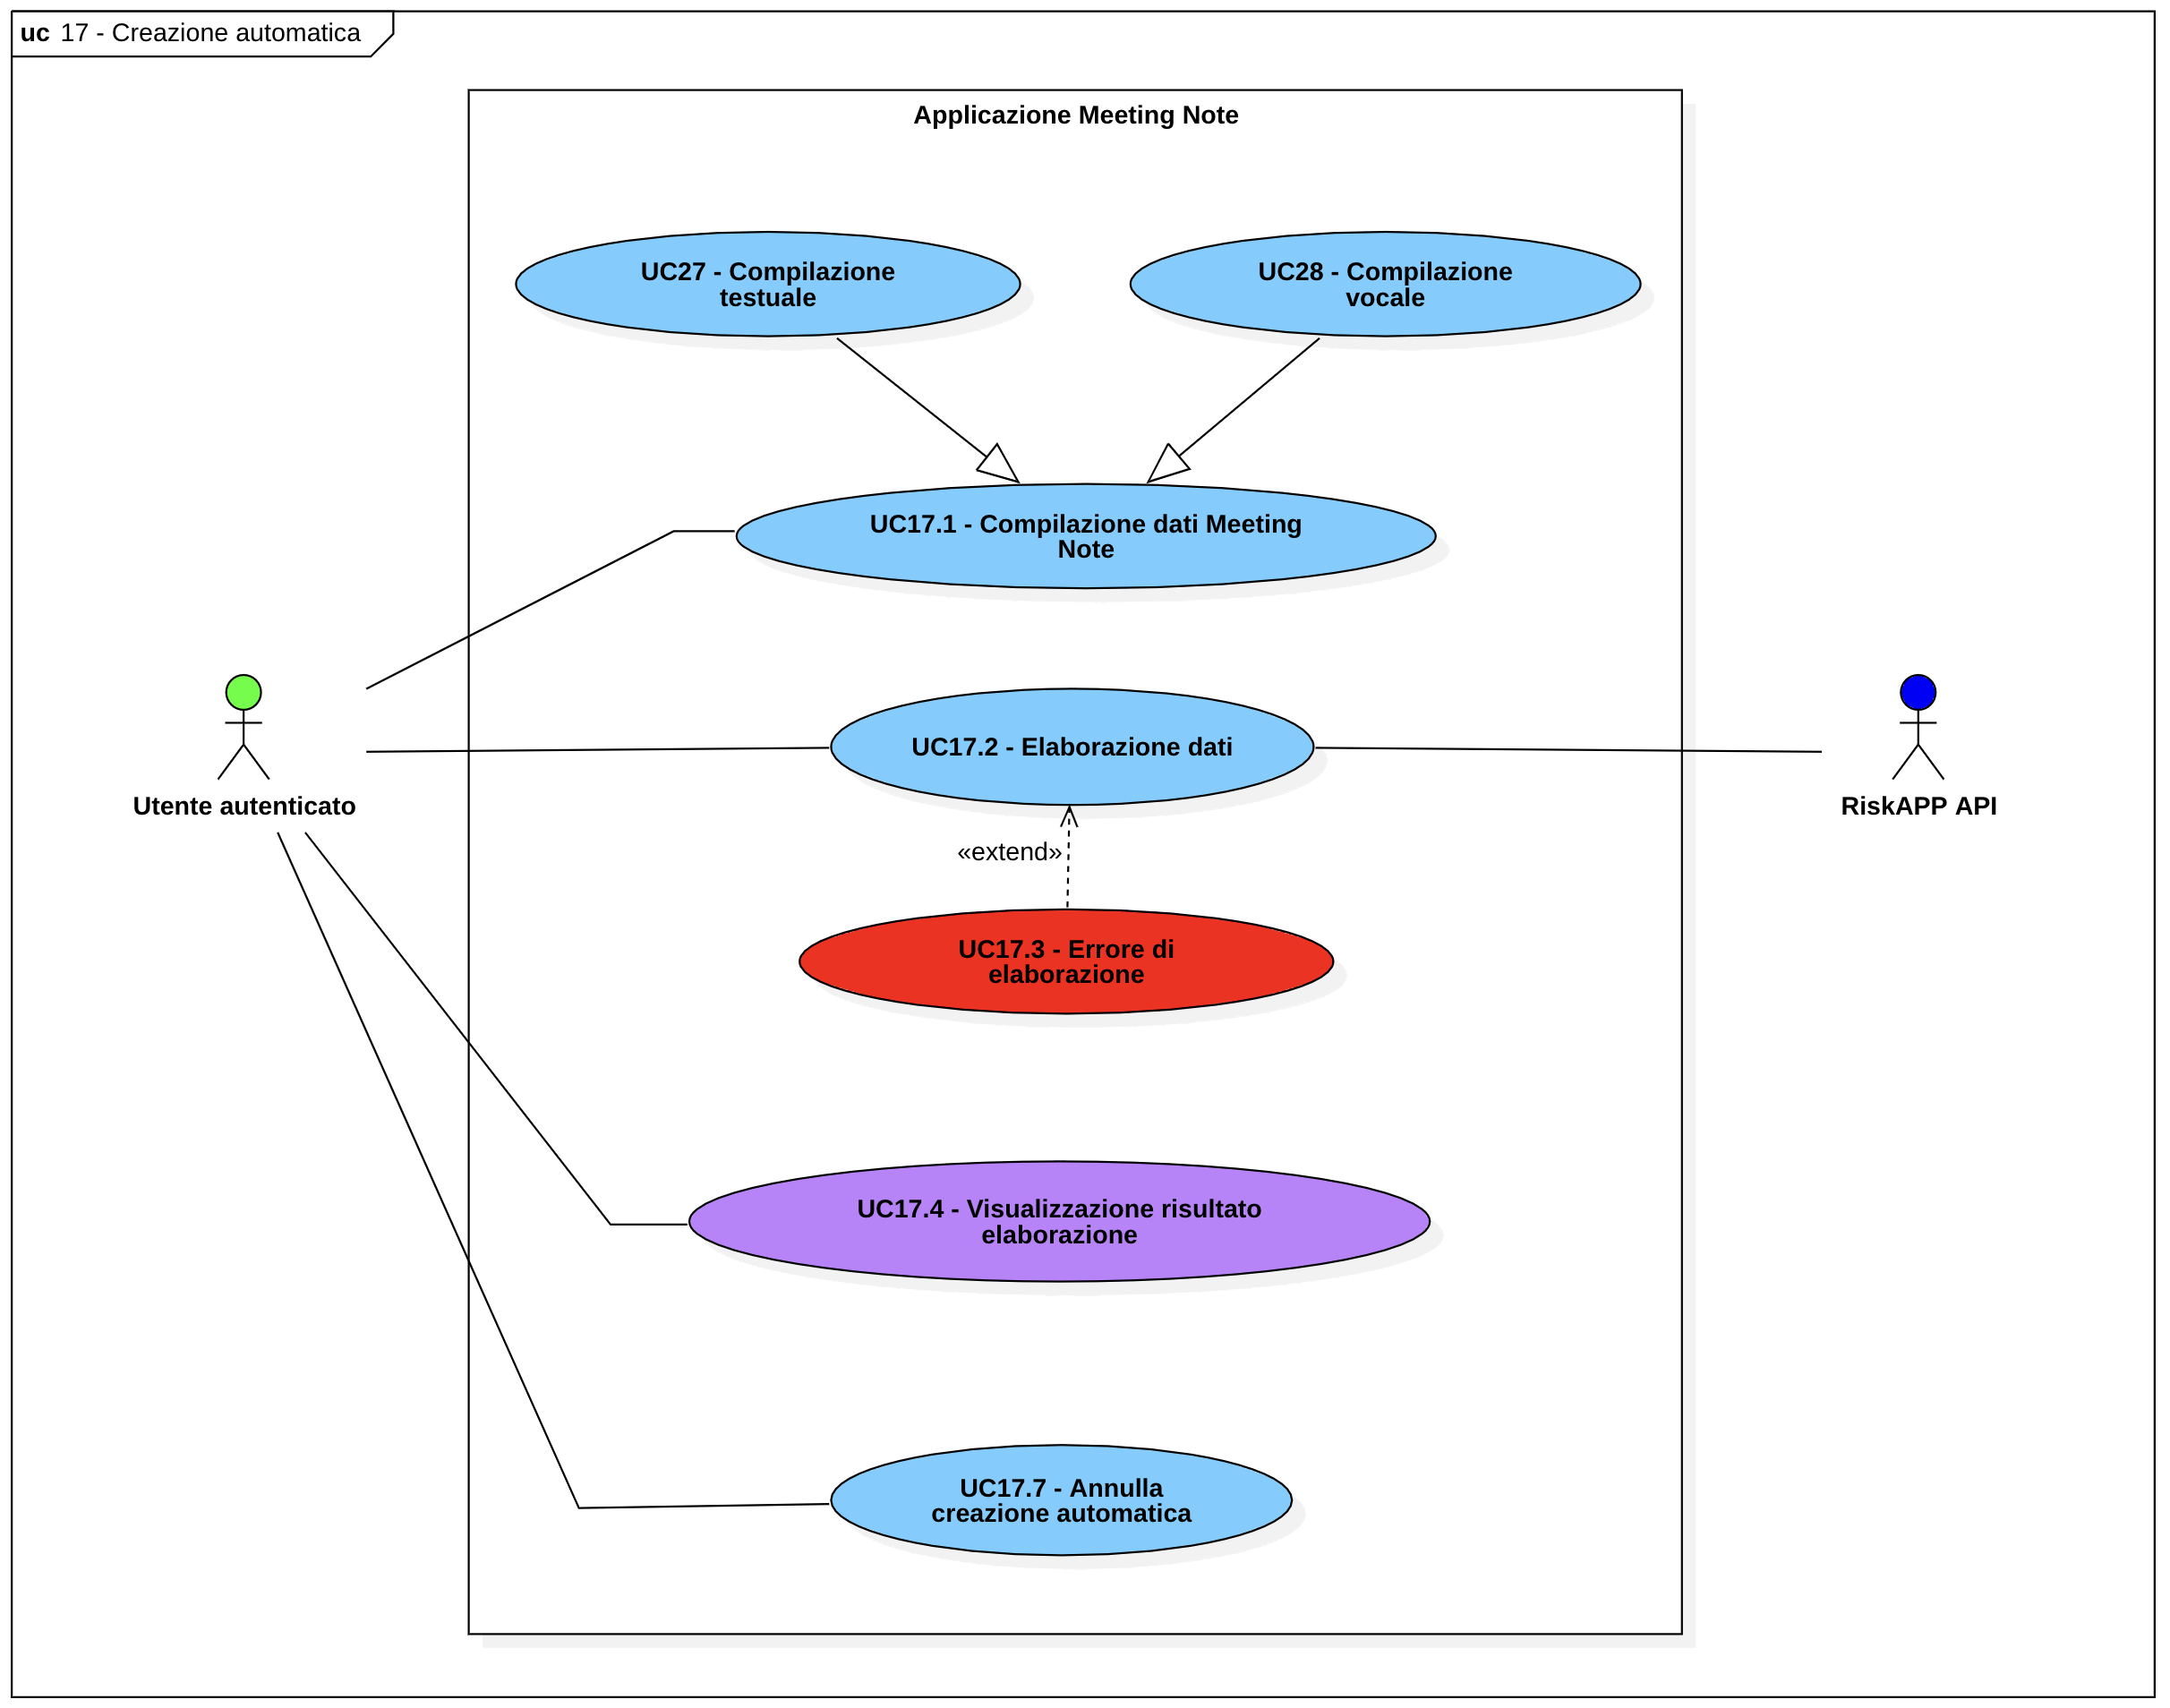
\includegraphics[width=1.0\columnwidth]{usecase/9-uc} 
    \caption{Use Case - Creazione automatica}
    \label{fig:uc-meetingnote-create-automatic}
\end{figure}

\begin{usecase}{17.1}{Compilazione dati Meeting Note}
    \usecasemainactors{Utente autenticato}
    \usecasepre{L'utente vuole creare automaticamente una \gls{meetingnote}\glsoccur}
    \usecasedesc{L'utente compila i dati necessari per la creazione automatica di una \gls{meetingnote}\glsoccur sotto forma di una descrizione testuale.}
    \usecasepost{È stato scritto una breve descrizione testuale con i dati necessari per la creazione automatica di una \gls{meetingnote}\glsoccur}
    \usecaseimg{\ref{fig:uc-meetingnote-create-automatic}}
    \label{UC17.1}
\end{usecase}

\begin{usecase}{17.2}{Elaborazione dati}
    \usecasemainactors{Utente autenticato}
    \usecasesecondaryactors{\emph{RiskAPP API}}
    \usecasepre{L'utente ha compilato i dati necessari per la creazione automatica di una \gls{meetingnote}\glsoccur}
    \usecasedesc{Il testo viene elaborato da una algoritmo di \gls{iag}\glsoccur per estrapolare i dati (cliente, data e contenuto) per la creazione automatica di una \gls{meetingnote}\glsoccur.}
    \usecasepost{I dati (cliente, data e contenuto) per la creazione automatica di una \gls{meetingnote}\glsoccur sono stati estrapolati}
    \usecasealt{Se l'elaborazione fallisce, si verifica \hyperref[UC17.3]{UC17.3}}
    \usecaseimg{\ref{fig:uc-meetingnote-create-automatic}}
    \label{UC17.2}
\end{usecase}

\begin{usecase}{17.3}{Errore elaborazione dati}
    \usecasemainactors{Utente autenticato}
    \usecasesecondaryactors{\emph{RiskAPP API}}
    \usecasepre{L'utente ha compilato i dati necessari per la creazione automatica di una \gls{meetingnote}\glsoccur}
    \usecasedesc{L'elaborazione dei dati per la creazione di una \gls{meetingnote}\glsoccur fallisce e l'utente viene informato dell'errore; le motivazioni possono essere le seguenti:
        \begin{itemize}
            \item l'algoritmo non è stato in grado di estrapolare i dati;
            \item il sistema non è raggiungibile;
            \item token di autenticazione scaduto;
            \item connessione ad internet assente.
        \end{itemize}}
    \usecasepost{I dati per la creazione automatica di una \gls{meetingnote}\glsoccur non sono stati estrapolati}
    \usecaseimg{\ref{fig:uc-meetingnote-create-automatic}}
    \label{UC17.3}
\end{usecase}

\begin{usecase}{17.4}{Visualizzazione risultato elaborazione}
    \usecasemainactors{Utente autenticato}
    \usecasepre{L'algoritmo ha estrapolato i dati per la creazione di una \gls{meetingnote}\glsoccur}
    \usecasedesc{L'utente vuole visualizzare i dati estrapolati dall'algoritmo per la creazione automatica di una \gls{meetingnote}\glsoccur, per accertarsi della loro correttezza.}
    \usecasepost{Sono visualizzabili i dati estrapolati dall'algoritmo per la creazione di una \gls{meetingnote}\glsoccur}
    \usecaseimg{\ref{fig:uc-meetingnote-create-automatic}}
    \label{UC17.4}
\end{usecase}

\newpage

\begin{figure}[!h] 
    \centering 
    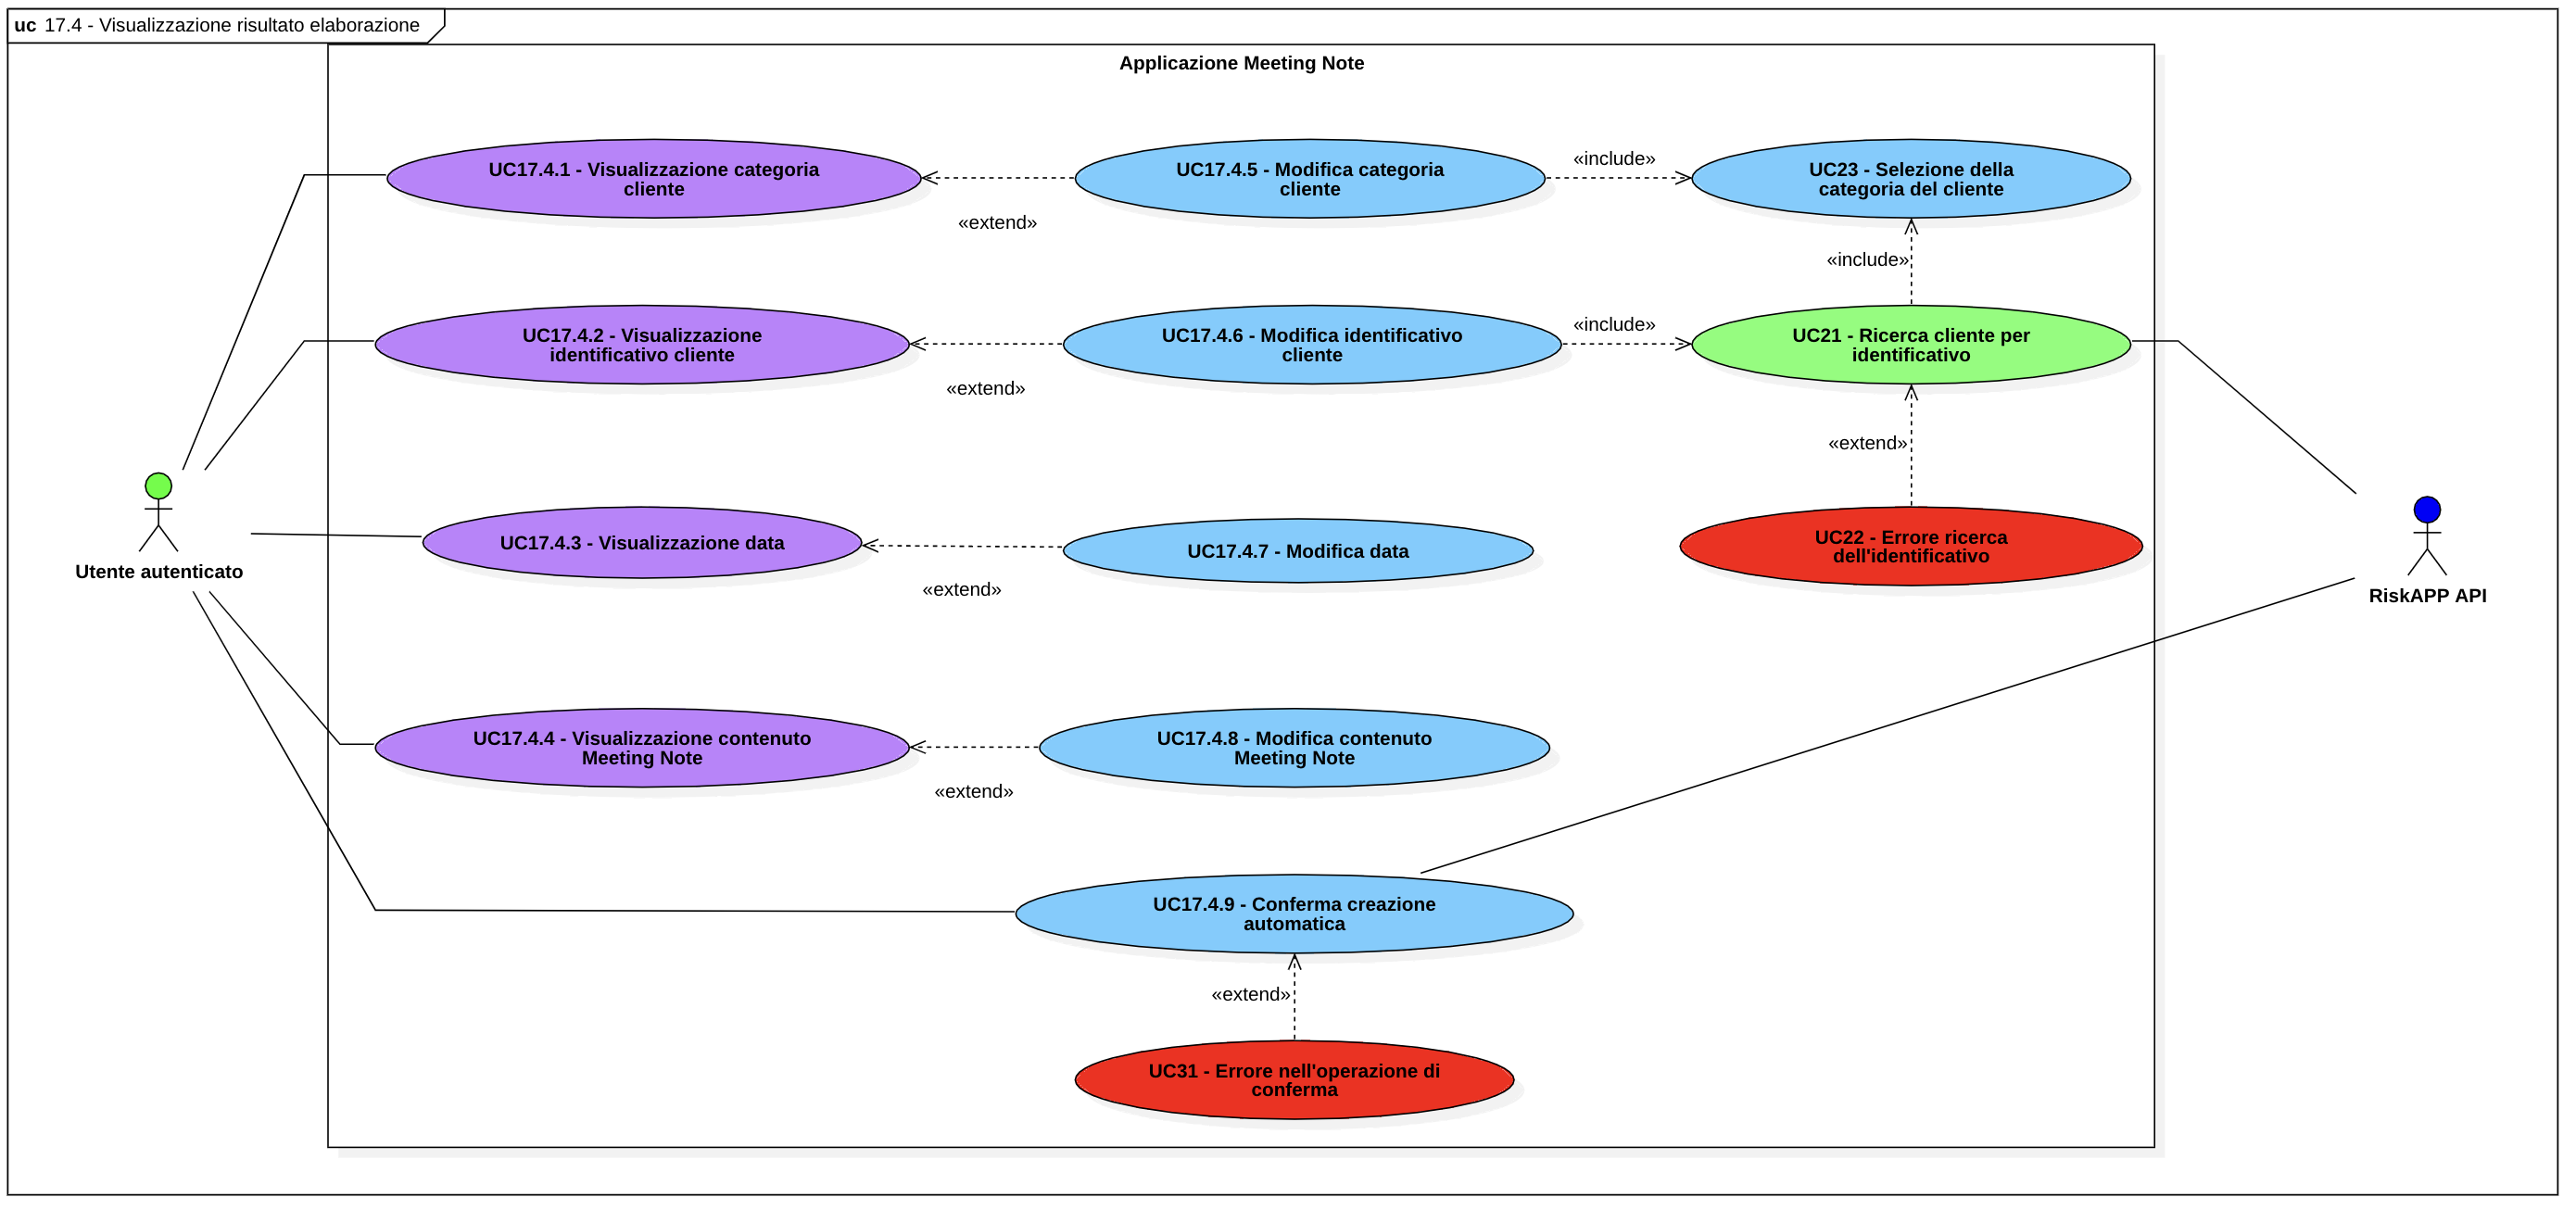
\includegraphics[width=1.0\columnwidth]{usecase/10-uc} 
    \caption{Use Case - Visualizzazione risultato elaborazione}
    \label{fig:uc-meetingnote-create-automatic-result}
\end{figure}

\begin{usecase}{17.4.1}{Visualizzazione categoria cliente}
    \usecasemainactors{Utente autenticato}
    \usecasepre{L'utente visualizza i dati estrapolati dall'algoritmo}
    \usecasedesc{L'utente vuole visualizzare la categoria del \gls{cliente}\glsoccur estrapolato}
    \usecasepost{È visualizzabile la categoria del \gls{cliente}\glsoccur estrapolato}
    \usecaseimg{\ref{fig:uc-meetingnote-create-automatic-result}}
    \label{UC17.4.1}
\end{usecase}

\begin{usecase}{17.4.2}{Visualizzazione identificativo cliente}
    \usecasemainactors{Utente autenticato}
    \usecasepre{L'utente visualizza i dati estrapolati dall'algoritmo}
    \usecasedesc{L'utente vuole visualizzare del \gls{cliente}\glsoccur estrapolato}
    \usecasepost{È visualizzabile l'identificativo del \gls{cliente}\glsoccur estrapolato}
    \usecaseimg{\ref{fig:uc-meetingnote-create-automatic-result}}
    \label{UC17.4.2}
\end{usecase}

\begin{usecase}{17.4.3}{Visualizzazione data}
    \usecasemainactors{Utente autenticato}
    \usecasepre{L'utente visualizza i dati estrapolati dall'algoritmo}
    \usecasedesc{L'utente vuole visualizzare la data estrapolata}
    \usecasepost{È visualizzabile la data estrapolata}
    \usecaseimg{\ref{fig:uc-meetingnote-create-automatic-result}}
    \label{UC17.4.3}
\end{usecase}

\begin{usecase}{17.4.4}{Visualizzazione il contenuto Meeting Note}
    \usecasemainactors{Utente autenticato}
    \usecasepre{L'utente visualizza i dati estrapolati dall'algoritmo}
    \usecasedesc{L'utente vuole visualizzare il contenuto estrapolato}
    \usecasepost{È visualizzabile il contenuto estrapolato}
    \usecaseimg{\ref{fig:uc-meetingnote-create-automatic-result}}
    \label{UC17.4.4}
\end{usecase}

\begin{usecase}{17.4.5}{Modifica categoria cliente}
    \usecasemainactors{Utente autenticato}
    \usecasepre{L'utente visualizza la categoria del \gls{cliente}\glsoccur estrapolato}
    \usecasedesc{L'utente modifica la categoria del \gls{cliente}\glsoccur}
    \usecasepost{La categoria del \gls{cliente}\glsoccur è stato modificato}
    \usecaseimg{\ref{fig:uc-meetingnote-create-automatic-result}}
    \label{15.4.5}
\end{usecase}

\begin{usecase}{17.4.6}{Modifica identificativo cliente}
    \usecasemainactors{Utente autenticato}
    \usecasepre{L'utente visualizza l'identificativo del \gls{cliente}\glsoccur estrapolato}
    \usecasedesc{L'utente modifica l'identificativo del \gls{cliente}\glsoccur}
    \usecasepost{L'identificativo del \gls{cliente}\glsoccur è stato modificato}
    \usecaseimg{\ref{fig:uc-meetingnote-create-automatic-result}}
    \label{15.4.6}
\end{usecase}

\begin{usecase}{17.4.7}{Modifica data}
    \usecasemainactors{Utente autenticato}
    \usecasepre{L'utente visualizza la data estrapolata}
    \usecasedesc{L'utente modifica la data}
    \usecasepost{La data è stata modificata}
    \usecaseimg{\ref{fig:uc-meetingnote-create-automatic-result}}
    \label{15.4.7}
\end{usecase}

\begin{usecase}{17.4.8}{Modifica contenuto Meeting Note}
    \usecasemainactors{Utente autenticato}
    \usecasepre{L'utente visualizza il contenuto estrapolato}
    \usecasedesc{L'utente modifica il contenuto}
    \usecasepost{Il contenuto è stato modificato}
    \usecaseimg{\ref{fig:uc-meetingnote-create-automatic-result}}
    \label{15.4.8}
\end{usecase}

\begin{usecase}{17.4.9}{Conferma creazione automatica}
    \usecasemainactors{Utente autenticato}
    \usecasepre{L'utente vuole creare automaticamente una \gls{meetingnote}\glsoccur}
    \usecasedesc{L'utente conferma la creazione automatica di una \gls{meetingnote}\glsoccur.}
    \usecasepost{Una nuova \gls{meetingnote}\glsoccur è stata creata automaticamente}
    \usecasealt{Se la conferma fallisce, si verifica \hyperref[UC31]{UC31}}
    \usecaseimg{\ref{fig:uc-meetingnote-create-automatic-result}}
    \label{15.4.9}
\end{usecase}

\begin{usecase}{17.5}{Annulla creazione automatica}
    \usecasemainactors{Utente autenticato}
    \usecasepre{L'utente é in fase di creazione automatica di una \gls{meetingnote}\glsoccur}
    \usecasedesc{L'utente annulla la creazione automatica di una \gls{meetingnote}\glsoccur.}
    \usecasepost{Non è stata creata una nuova \gls{meetingnote}\glsoccur}
    \usecaseimg{\ref{fig:uc-meetingnote-create-automatic}}
    \label{UC17.5}
\end{usecase}

\newpage

\begin{figure}[!h] 
    \centering 
    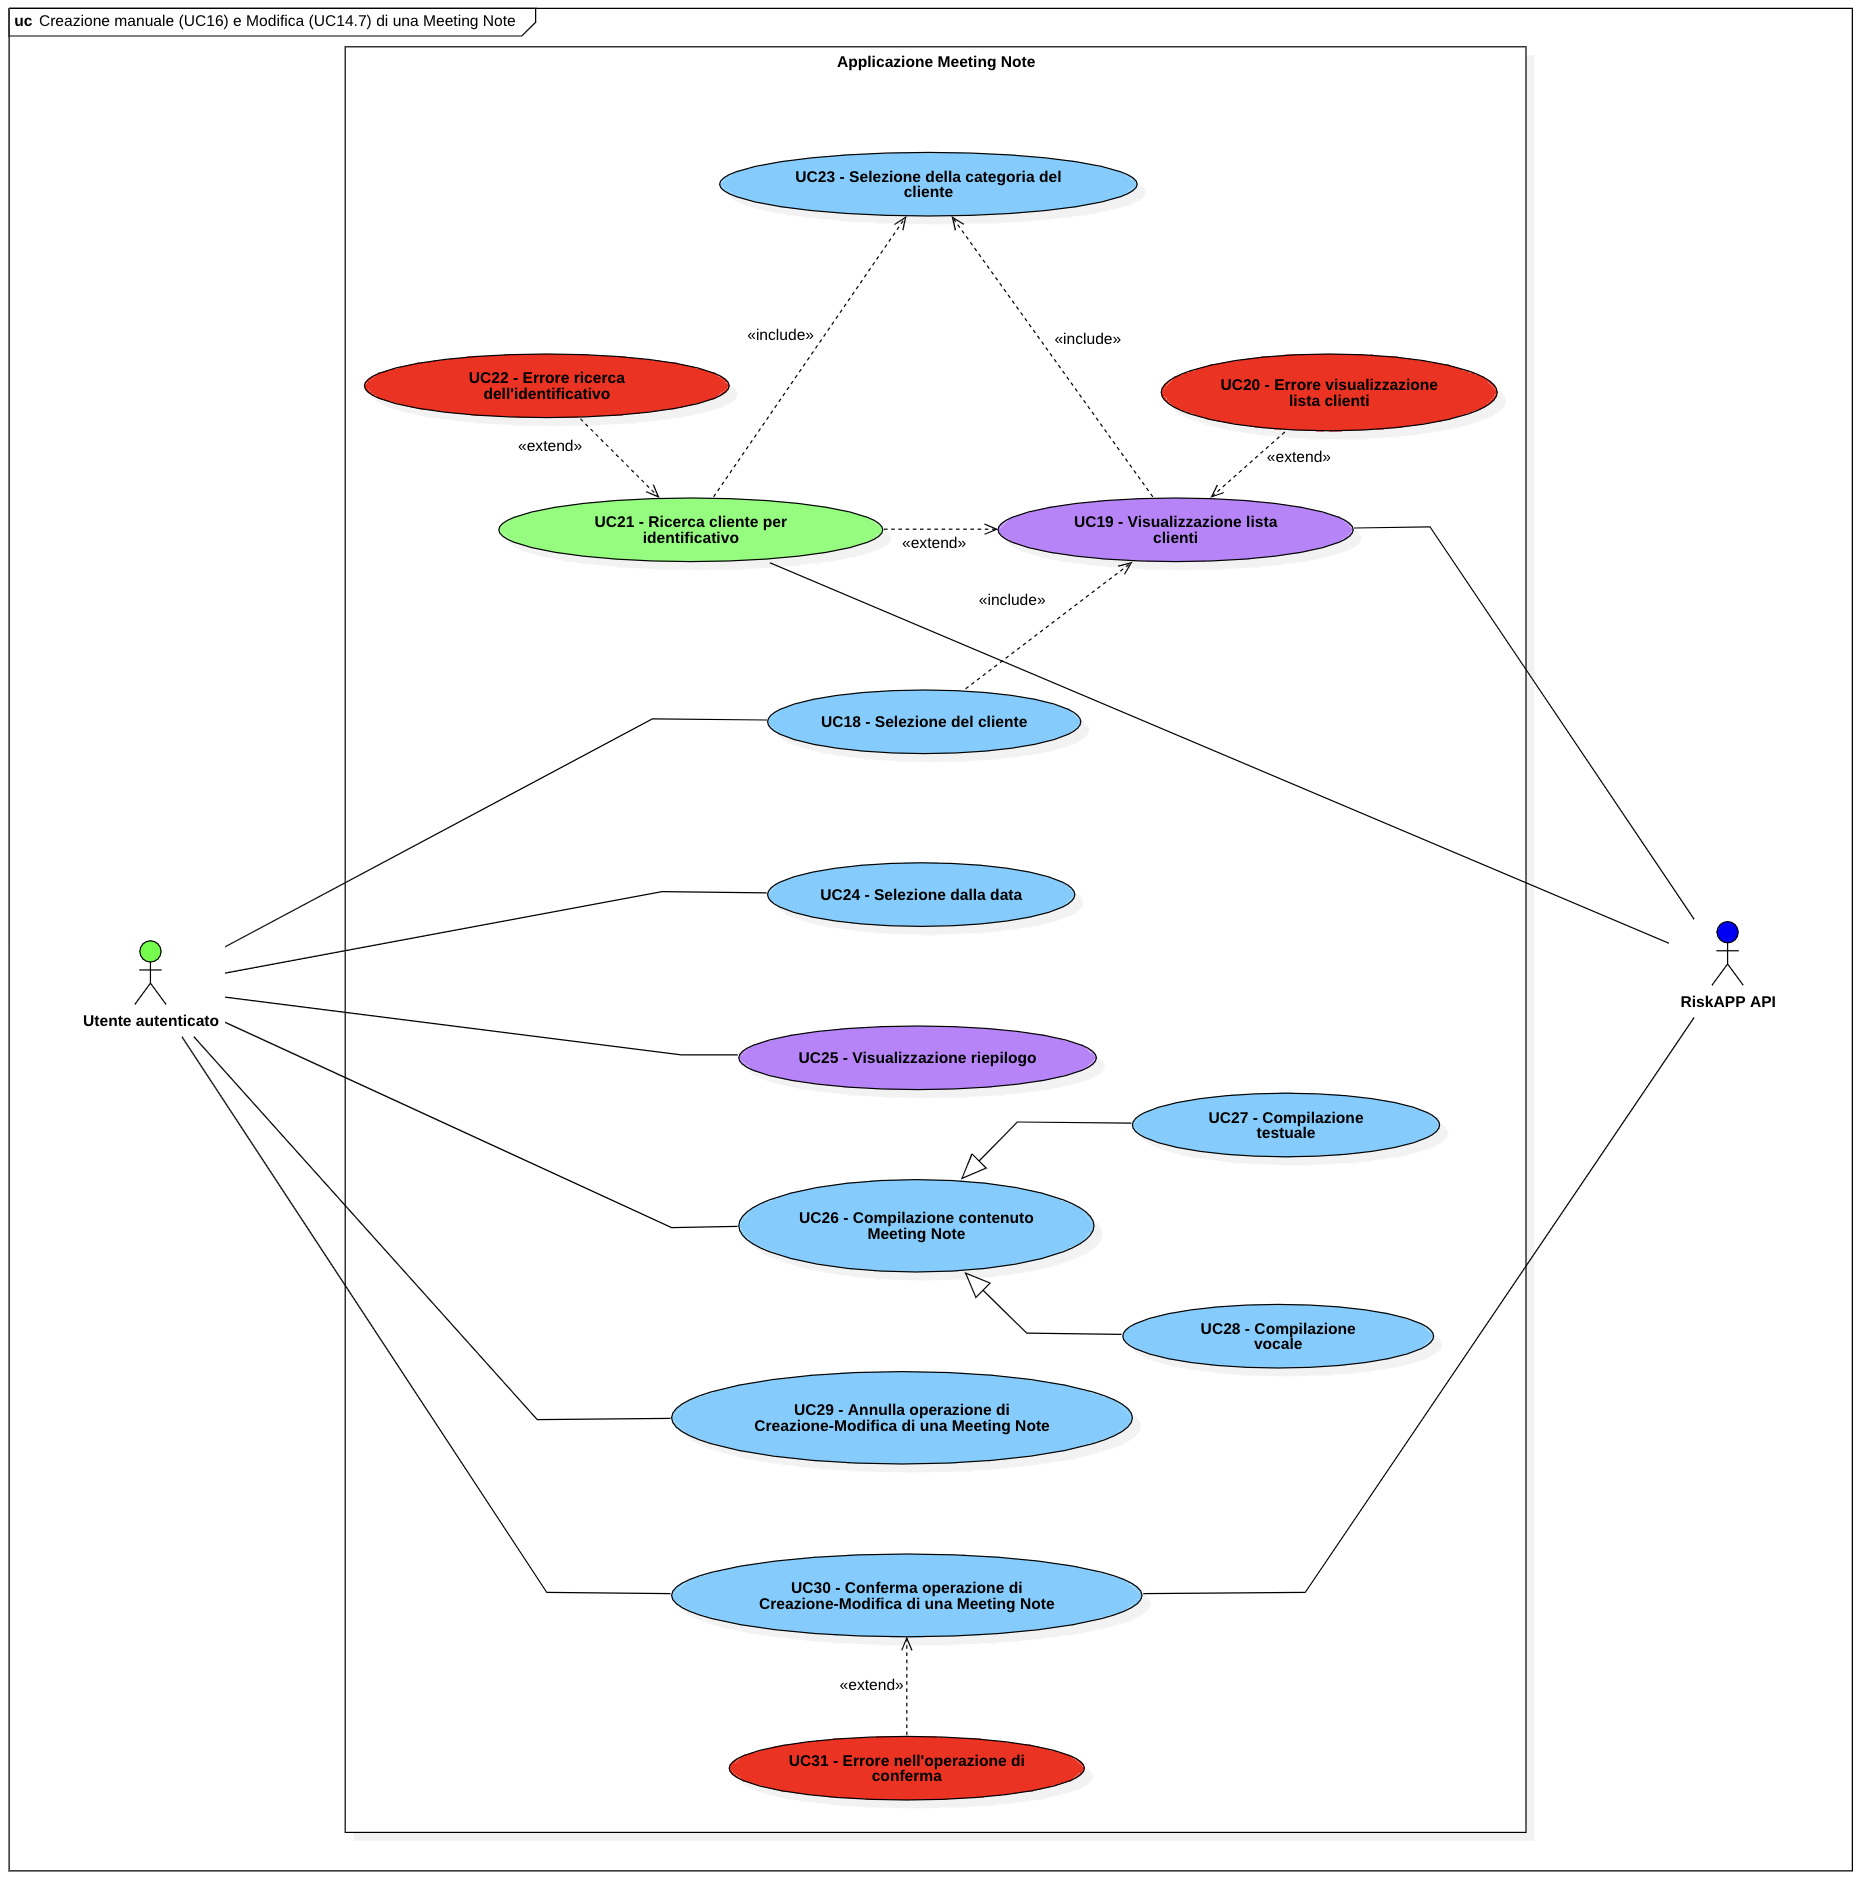
\includegraphics[width=1.0\columnwidth]{usecase/8-uc} 
    \caption{Use Case - Creazione manuale (\hyperref[UC16]{UC16}) e Modifica (\hyperref[UC14.7]{UC14.7}) di una Meeting Note}
    \label{fig:uc-meetingnote-create-manual}
\end{figure}

\noindent Per la creazione manuale (\hyperref[UC16]{UC16}) e modifica (\hyperref[UC14.7]{UC14.7}) di una \gls{meetingnote}\glsoccur sono stati individuati i seguenti \glspl{usecase}\glsoccur, che sono in comune tra le due funzionalità sopra citate, in quanto condividono la stessa sequenza di azioni, e dunque di attori principali, secondari, precondizioni e postcondizioni.

\begin{usecase}{18}{Selezione del cliente}
    \usecasemainactors{Utente autenticato}
    \usecasepre{L'utente vuole creare manualmente o modificare una \gls{meetingnote}\glsoccur}
    \usecasedesc{L'utente deve selezionare un \gls{cliente}\glsoccur per la creazione o la modifica di una \gls{meetingnote}\glsoccur.}
    \usecasepost{Il \gls{cliente}\glsoccur è stato selezionato}
    \usecaseimg{\ref{fig:uc-meetingnote-create-manual}}
    \label{UC18}
\end{usecase}

\begin{usecase}{19}{Visualizzazione lista clienti}
    \usecasemainactors{Utente autenticato}
    \usecasesecondaryactors{\emph{RiskAPP API}}
    \usecasepre{L'utente ha selezionato la categoria del \gls{cliente}\glsoccur}
    \usecasedesc{L'utente vuole visualizzare la lista di tutti i \glspl{cliente}\glsoccur della categoria selezionata.}
    \usecasepost{È visualizzabile la lista dei \glspl{cliente}\glsoccur filtrata per categoria}
    \usecasealt{Se la visualizzazione fallisce, si verifica \hyperref[UC20]{UC20}}
    \usecaseimg{\ref{fig:uc-meetingnote-create-manual}}
    \label{UC19}
\end{usecase}

\begin{usecase}{20}{Errore visualizzazione lista clienti}
    \usecasemainactors{Utente autenticato}
    \usecasesecondaryactors{\emph{RiskAPP API}}
    \usecasepre{L'utente ha selezionato la categoria del \gls{cliente}\glsoccur}
    \usecasedesc{La visualizzazione della lista dei \glspl{cliente}\glsoccur fallisce e l'utente viene informato dell'errore; le motivazioni possono essere le seguenti:
        \begin{itemize}
            \item la lista è vuota;
            \item il sistema non è raggiungibile;
            \item token di autenticazione scaduto;
            \item connessione ad internet assente.
        \end{itemize}}
    \usecasepost{Non è visualizzabile la lista dei \glspl{cliente}\glsoccur filtrata per categoria}
    \usecaseimg{\ref{fig:uc-meetingnote-create-manual}}
    \label{UC20}
\end{usecase}

\begin{usecase}{21}{Ricerca cliente per identificativo}
    \usecasemainactors{Utente autenticato}
    \usecasesecondaryactors{\emph{RiskAPP API}}
    \usecasepre{L'utente ha selezionato la categoria del \gls{cliente}\glsoccur}
    \usecasedesc{L'utente effettua una ricerca per identificativo del \gls{cliente}\glsoccur.}
    \usecasepost{L'identificativo del \gls{cliente}\glsoccur è stato trovato}
    \usecasealt{Se la ricerca fallisce, si verifica \hyperref[UC22]{UC22}}
    \usecaseimg{\ref{fig:uc-meetingnote-create-manual}}
    \label{UC21}
\end{usecase}

\begin{usecase}{22}{Errore ricerca dell'identificativo}
    \usecasemainactors{Utente autenticato}
    \usecasesecondaryactors{\emph{RiskAPP API}}
    \usecasepre{L'utente ha effettuato una ricerca per identificativo del \gls{cliente}\glsoccur}
    \usecasedesc{La ricerca dell'identificativo del \gls{cliente}\glsoccur fallisce e l'utente viene informato dell'errore; le motivazioni possono essere le seguenti:
        \begin{itemize}
            \item la lista risultante è vuota;
            \item il sistema non è raggiungibile;
            \item token di autenticazione scaduto;
            \item connessione ad internet assente.
        \end{itemize}}
    \usecasepost{L'identificativo del \gls{cliente}\glsoccur non è stato trovato}
    \usecaseimg{\ref{fig:uc-meetingnote-create-manual}}
    \label{UC22}
\end{usecase}

\begin{usecase}{23}{Selezione della categoria del cliente}
    \usecasemainactors{Utente autenticato}
    \usecasepre{L'utente è in fase di creazione o modifica}
    \usecasedesc{L'utente seleziona la categoria del \gls{cliente}\glsoccur per filtrare la lista dei \glspl{cliente}\glsoccur e/o la ricerca dell'identificativo.}
    \usecasepost{La categoria del \gls{cliente}\glsoccur è stata selezionata}
    \usecaseimg{\ref{fig:uc-meetingnote-create-manual}}
    \label{UC23}
\end{usecase}

\begin{usecase}{24}{Selezione della data}
    \usecasemainactors{Utente autenticato}
    \usecasepre{L'utente vuole creare manualmente o modificare una \gls{meetingnote}\glsoccur}
    \usecasedesc{L'utente deve selezionare una data, in cui è avvenuto l'incontro, per la creazione o la modifica di una \gls{meetingnote}\glsoccur.}
    \usecasepost{La data dell'incontro è stata selezionata}
    \usecaseimg{\ref{fig:uc-meetingnote-create-manual}}
    \label{UC24}
\end{usecase}

\begin{usecase}{25}{Visualizzazione riepilogo}
    \usecasemainactors{Utente autenticato}
    \usecasepre{L'utente ha selezionato un \gls{cliente}\glsoccur e una data}
    \usecasedesc{Viene visualizzato il riepilogo dei dati selezionati.}
    \usecasepost{È visualizzabile il riepilogo dei dati selezionati}
    \usecaseimg{\ref{fig:uc-meetingnote-create-manual}}
    \label{UC25}
\end{usecase}

\newpage

\begin{figure}[!h] 
    \centering 
    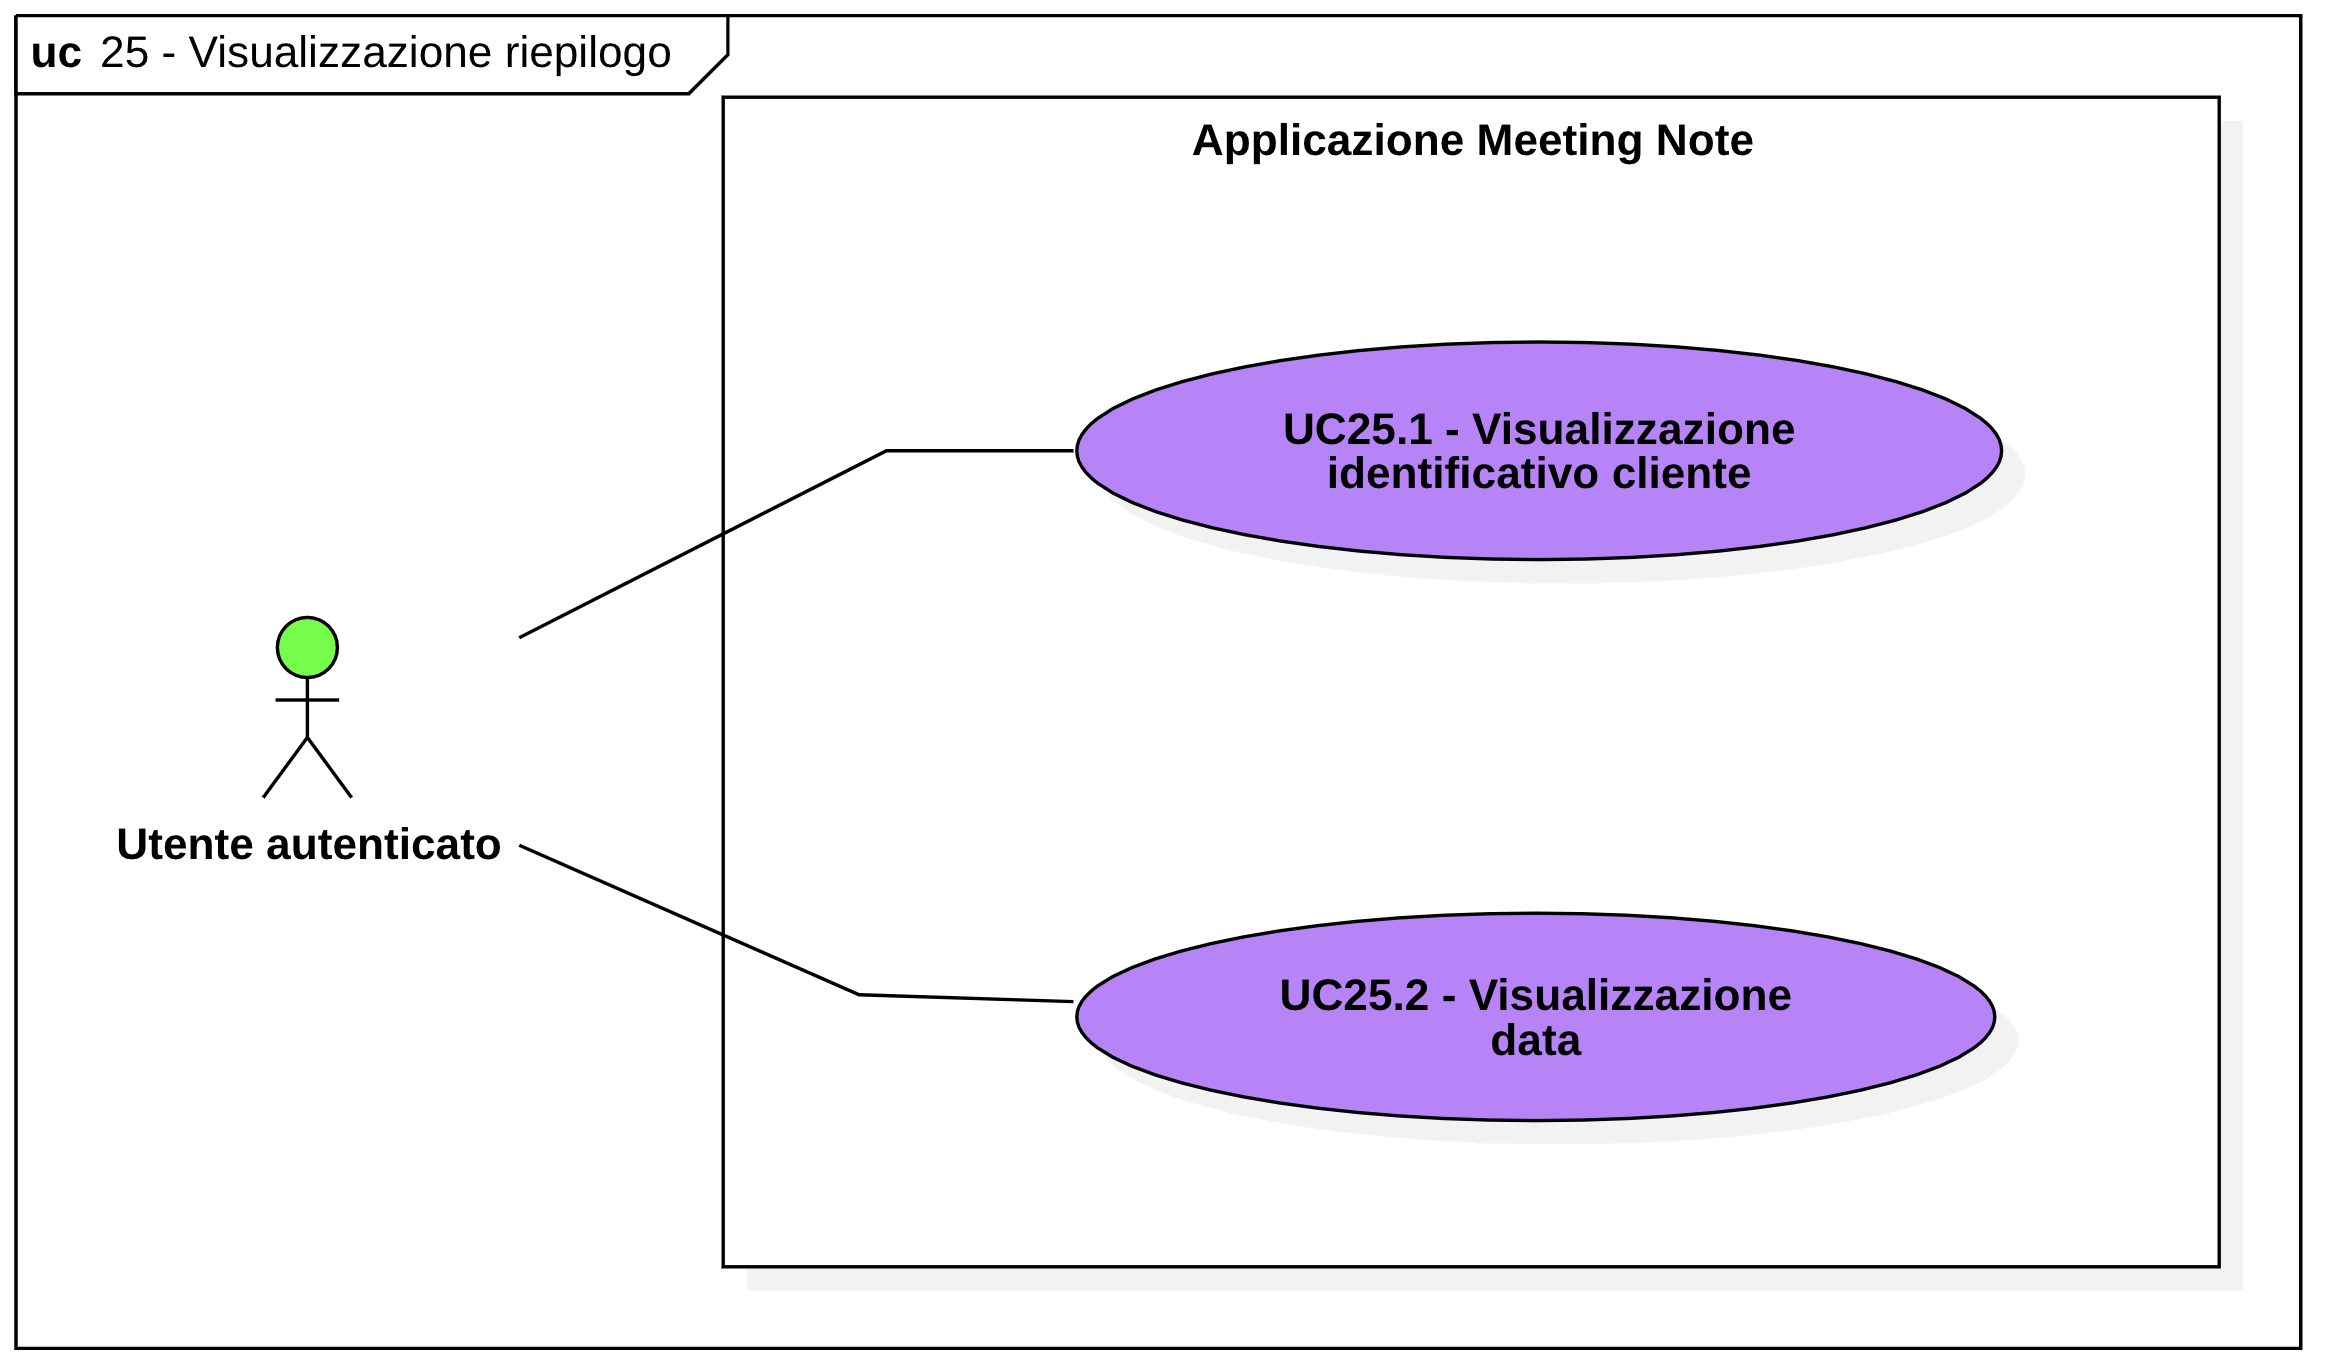
\includegraphics[width=1.0\columnwidth]{usecase/11-uc} 
    \caption{Use Case - Visualizzazione riepilogo}
    \label{fig:uc-meetingnote-create-manual-result}
\end{figure}

\begin{usecase}{25.1}{Visualizzazione identificativo cliente}
    \usecasemainactors{Utente autenticato}
    \usecasepre{L'utente visualizza il riepilogo}
    \usecasedesc{Viene visualizzato l'identificativo del \gls{cliente}\glsoccur selezionato.}
    \usecasepost{È visualizzabile l'identificativo del \gls{cliente}\glsoccur selezionato}
    \usecaseimg{\ref{fig:uc-meetingnote-create-manual-result}}
    \label{UC25.1}
\end{usecase}

\begin{usecase}{25.2}{Visualizzazione data}
    \usecasemainactors{Utente autenticato}
    \usecasepre{L'utente visualizza il riepilogo}
    \usecasedesc{Viene visualizzata la data selezionata.}
    \usecasepost{È visualizzabile la data selezionata}
    \usecaseimg{\ref{fig:uc-meetingnote-create-manual-result}}
    \label{UC25.2}
\end{usecase}

\begin{usecase}{26}{Compilazione contenuto Meeting Note}
    \usecasemainactors{Utente autenticato}
    \usecasepre{L'utente vuole creare manualmente o modificare una \gls{meetingnote}\glsoccur}
    \usecasedesc{L'utente deve compilare il contenuto della \gls{meetingnote}\glsoccur.}
    \usecasepost{Il contenuto della \gls{meetingnote}\glsoccur è compilato}
    \usecaseimg{\ref{fig:uc-meetingnote-create-manual}}
    \label{UC26}
\end{usecase}

\begin{usecase}{27}{Compilazione testuale}
    \usecasemainactors{Utente autenticato}
    \usecasepre{L'utente deve compilare il contenuto della \gls{meetingnote}\glsoccur}
    \usecasedesc{L'utente deve compilare il contenuto della \gls{meetingnote}\glsoccur con l'ausilio della tastiera.}
    \usecasepost{Il contenuto della \gls{meetingnote}\glsoccur è stato compilato con l'ausilio della tastiera}
    \usecaseimg{\ref{fig:uc-meetingnote-create-manual}}
    \label{UC27}
\end{usecase}

\begin{usecase}{28}{Compilazione vocale}
    \usecasemainactors{Utente autenticato}
    \usecasepre{L'utente deve compilare il contenuto della \gls{meetingnote}\glsoccur}
    \usecasedesc{L'utente deve compilare il contenuto della \gls{meetingnote}\glsoccur attraverso la dettatura vocale.}
    \usecasepost{Il contenuto della \gls{meetingnote}\glsoccur è stato compilato attraverso la dettatura vocale}
    \usecaseimg{\ref{fig:uc-meetingnote-create-manual}}
    \label{UC28}
\end{usecase}

\begin{usecase}{29}{Annulla operazione di Creazione-Modifica di una Meeting Note}
    \usecasemainactors{Utente autenticato}
    \usecasepre{L'utente ha selezionato: \gls{cliente}\glsoccur, data e compilato il contenuto della \gls{meetingnote}\glsoccur}
    \usecasedesc{L'utente vuole annullare l'operazione di creazione o modifica di una \gls{meetingnote}\glsoccur.}
    \usecasepost{L'operazione di creazione o modifica di una \gls{meetingnote}\glsoccur è annullata}
    \usecaseimg{\ref{fig:uc-meetingnote-create-manual}}
    \label{UC29}
\end{usecase}

\begin{usecase}{30}{Conferma operazione di Creazione-Modifica di una Meeting Note}
    \usecasemainactors{Utente autenticato}
    \usecasesecondaryactors{\emph{RiskAPP API}}
    \usecasepre{L'utente ha selezionato: \gls{cliente}\glsoccur, data e compilato il contenuto della \gls{meetingnote}\glsoccur}
    \usecasedesc{L'utente vuole confermare l'operazione di creazione o modifica di una \gls{meetingnote}\glsoccur.}
    \usecasepost{L'operazione di creazione o modifica di una \gls{meetingnote}\glsoccur è confermata}
    \usecasealt{Se la conferma fallisce, si verifica \hyperref[UC31]{UC31}}
    \usecaseimg{\ref{fig:uc-meetingnote-create-manual}}
    \label{UC30}
\end{usecase}

\begin{usecase}{31}{Errore nell'operazione di conferma}
    \usecasemainactors{Utente autenticato}
    \usecasesecondaryactors{\emph{RiskAPP API}}
    \usecasepre{L'utente ha confermato l'operazione di creazione o modifica di una \gls{meetingnote}\glsoccur}
    \usecasedesc{La conferma dell'operazione di creazione o modifica della \gls{meetingnote}\glsoccur fallisce e l'utente viene informato dell'errore; le motivazioni possono essere le seguenti:
        \begin{itemize}
            \item il sistema non è raggiungibile;
            \item token di autenticazione scaduto;
            \item connessione ad internet assente.
        \end{itemize}}
    \usecasepost{La conferma dell'operazione di creazione o modifica di una \gls{meetingnote}\glsoccur è fallita}
    \usecaseimg{\ref{fig:uc-meetingnote-create-manual}}
    \label{UC31}
\end{usecase}

\clearpage

\section{Tracciamento dei requisiti}

Da un'attenta analisi dei requisiti e dei casi d'uso effettuata sul progetto è stata stilata la tabella che traccia i requisiti.\\
Sono stati individuati diversi tipi di requisiti e si è quindi fatto utilizzo di un codice identificativo per distinguerli.\\
Il codice dei requisiti è così strutturato R(F/Q/V)(N/D/O) dove:
\begin{enumerate}
	\item[R =] requisito
    \item[F =] funzionale
    \item[Q =] qualitativo
    \item[V =] di vincolo
    \item[N =] obbligatorio (necessario)
    \item[D =] desiderabile
    \item[Z =] opzionale
\end{enumerate}

Di seguito sono riportate le tabelle che raccolgono, per tipologia, i requisiti individuati.\\
\begin{itemize}
    \item \textbf{Requisiti funzionali}: descrivono le funzionalità offerte dal prodotto software. Si faccia riferimento alle tabelle \ref{tab:requisiti-funzionali-1}, \ref{tab:requisiti-funzionali-2}, \ref{tab:requisiti-funzionali-3}, \ref{tab:requisiti-funzionali-4};
    \item \textbf{Requisiti qualitativi}: descrivono le caratteristiche qualitative che il prodotto software deve possedere. Si faccia riferimento alla tabella \ref{tab:requisiti-qualitativi};
    \item \textbf{Requisiti di vincolo}: descrivono i vincoli che il prodotto software deve rispettare. Si faccia riferimento alla tabella \ref{tab:requisiti-vincolo}.
\end{itemize}

\clearpage

\begin{table}%
\caption{Tabella del tracciamento dei requisti funzionali - 1}
\label{tab:requisiti-funzionali-1}
\begin{tabularx}{\textwidth}{lXl}
\hline\hline
\textbf{Requisito} & \textbf{Descrizione} & \textbf{Use Case}\\
\hline
RFN-1 \label{RFN-1} & Il sistema permette di effettuare l'autenticazione & \hyperref[UC01]{UC01} \\
\hline
RFN-2 \label{RFN-2} & Il sistema permette di inserire le credenziali (\emph{username} e \emph{password}) per effettuare l'autenticazione & \hyperref[UC02]{UC02} \\
\hline
RFN-3 \label{RFN-3} & Il sistema permette il riconoscimento biometrico per effettuare l'autenticazione & \hyperref[UC03]{UC03} \\
\hline
% INSERIRE RFN CHE SPECIFICA IL FALLIMENTO DELL'AUTENTICAZIONE (IN TEORIA CI SONO ALTRI CASI SIMILI, DA SPECIFICARE ANALOGAMENTE)
RFN-4 \label{RFN-4} & Il sistema deve notificare l'utente in caso di inserimento di credenziali errate & \hyperref[UC04]{UC04} \\ % \hyperref[UC08.8]{UC08.8}
\hline
RFN-5 \label{RFN-5} & Il sistema deve notificare l'utente in caso in cui il sistema, ovvero la piattaforma \emph{RiskAPP} non sia raggiungibile & \hyperref[UC04]{UC04} \\ %, \hyperref[UC06]{UC06}, \hyperref[UC07.6]{UC07.6}, \hyperref[UC08.8]{UC08.8}, \hyperref[UC09]{UC09}, \hyperref[UC13]{UC13}, \hyperref[UC14.6]{UC14.6}, \hyperref[UC17.3]{UC17.3}, \hyperref[UC20]{UC20}, \hyperref[UC22]{UC22}, \hyperref[UC31]{UC31} 
\hline
RFN-6 \label{RFN-6} & Il sistema deve permettere all'utente, in caso in cui il riconoscimento biometrico fallisca, di poter inserire le credenziali manualmente & \hyperref[UC04]{UC04} \\
\hline
RFN-7 \label{RFN-7} & Il sistema deve notificare l'utente in caso di connessione internet assente & \hyperref[UC04]{UC04} \\ %, \hyperref[UC06]{UC06}, \hyperref[UC07.6]{UC07.6}, \hyperref[UC08.8]{UC08.8}, \hyperref[UC09]{UC09}, \hyperref[UC13]{UC13}, \hyperref[UC14.6]{UC14.6}, \hyperref[UC17.3]{UC17.3}, \hyperref[UC20]{UC20}, \hyperref[UC22]{UC22}, \hyperref[UC31]{UC31} 
\hline
RFN-8 \label{RFN-8} & Il sistema permette di visualizzare la lista di \emph{Meeting Note} & \hyperref[UC05]{UC05} \\
\hline
RFN-9 \label{RFN-9} & Il sistema permette di visualizzare i clienti di ciascuna \emph{Meeting Note} nella lista & \hyperref[UC05.1]{UC05.1} \\
\hline
RFN-10 \label{RFN-10} & Il sistema permette di visualizzare la data dell'incontro di ciascuna \emph{Meeting Note} nella lista & \hyperref[UC05.2]{UC05.2} \\
\hline
RFN-11 \label{RFN-11} & Il sistema permette di visualizzare parzialmente il contenuto di ciascuna \emph{Meeting Note} nella lista & \hyperref[UC05.3]{UC05.3} \\
\hline
RFN-12 \label{RFN-12} & Il sistema deve notificare l'utente in caso la lista di \emph{Meeting Note} sia vuota & \hyperref[UC06]{UC06} \\
\hline
RFN-13 \label{RFN-13} & Il sistema deve notificare l'utente in caso sia scaduto il token di autenticazione & \hyperref[UC06]{UC06} \\ % \hyperref[UC07.6]{UC07.6}, \hyperref[UC08.8]{UC08.8}, \hyperref[UC09]{UC09}, \hyperref[UC13]{UC13}, \hyperref[UC14.6]{UC14.6}, \hyperref[UC17.3]{UC17.3}, \hyperref[UC20]{UC20}, \hyperref[UC22]{UC22}, \hyperref[UC31]{UC31}
\hline
RFN-14 \label{RFN-14} & Il sistema permette di effettuare una ricerca nella lista di \emph{Meeting Note} & \hyperref[UC07]{UC07} \\
\hline
RFN-15 \label{RFN-15} & Il sistema permette di effettuare una ricerca nella lista di \emph{Meeting Note} per identificativo del cliente & \hyperref[UC07.1]{UC07.1} \\
\hline
RFN-16 \label{RFN-16} & Il sistema permette di selezionare la categoria del cliente in modo da effettuare una ricerca nella lista di \emph{Meeting Note} per identificativo del cliente & \hyperref[UC07.2]{UC07.2} \\
\hline
RFN-17 \label{RFN-17} & Il sistema permette di effettuare una ricerca nella lista di \emph{Meeting Note} per data & \hyperref[UC07.3]{UC07.3} \\
\hline
RFN-18 \label{RFN-18} & Il sistema permette di effettuare una ricerca nella lista di \emph{Meeting Note} per data singola & \hyperref[UC07.4]{UC07.4} \\
\hline
RFN-19 \label{RFN-19} & Il sistema permette di effettuare una ricerca nella lista di \emph{Meeting Note} per intervallo di date & \hyperref[UC07.5]{UC07.5} \\
\hline
RFN-20 \label{RFN-20} & Il sistema permette di notificare l'utente in caso la lista filtrata sia vuota & \hyperref[UC07.6]{UC07.6} \\
\hline
RFN-21 \label{RFN-21} & Il sistema permette di visualizzare i dati personali dell'utente & \hyperref[UC08]{UC08} \\
\hline
\end{tabularx}
\end{table}

\clearpage

\begin{table}%
\caption{Tabella del tracciamento dei requisti funzionali - 2}
\label{tab:requisiti-funzionali-2}
\begin{tabularx}{\textwidth}{lXl}
\hline\hline
\textbf{Requisito} & \textbf{Descrizione} & \textbf{Use Case}\\
\hline
RFN-22 \label{RFN-22} & Il sistema permette di visualizzare il nome dell'utente & \hyperref[UC08.1]{UC08.1} \\
\hline
RFN-23 \label{RFN-23} & Il sistema permette di visualizzare il cognome dell'utente & \hyperref[UC08.2]{UC08.2} \\
\hline
RFN-24 \label{RFN-24} & Il sistema permette di visualizzare la email dell'utente & \hyperref[UC08.3]{UC08.3} \\
\hline
RFN-25 \label{RFN-25} & Il sistema permette di visualizzare l'avatar dell'utente & \hyperref[UC08.4]{UC08.4} \\
\hline
RFN-26 \label{RFN-26} & Il sistema permette di effettuare il logout & \hyperref[UC08.5]{UC08.5} \\
\hline
RFN-27 \label{RFN-27} & Il sistema permette di abilitare il riconoscimento biometrico & \hyperref[UC08.6]{UC08.6} \\
\hline
RFN-28 \label{RFN-28} & Il sistema permette di confermare l'abilitazione del riconoscimento biometrico, inserendo le credenziali (\emph{username} e \emph{password}) & \hyperref[UC08.7]{UC08.7} \\
\hline
RFN-29 \label{RFN-29} & Il sistema permette di notificare l'utente in caso in cui la conferma per l'abilitazione del riconoscimento biometrico non vada a buon fine & \hyperref[UC08.8]{UC08.8} \\
\hline
RFN-30 \label{RFN-30} & Il sistema permette di notificare l'utente se la visualizzazione dei dati personali fallisce & \hyperref[UC09]{UC09} \\
\hline
RFN-31 \label{RFN-31} & Il sistema permette di ordinare la lista di \emph{Meeting Note} & \hyperref[UC10]{UC10} \\
\hline
RFN-32 \label{RFN-32} & Il sistema permette di ordinare la lista di \emph{Meeting Note} per data meno recente & \hyperref[UC11]{UC11} \\
\hline
RFN-33 \label{RFN-33} & Il sistema permette di ordinare la lista di \emph{Meeting Note} per data più recente & \hyperref[UC12]{UC12} \\
\hline
RFN-34 \label{RFN-34} & Il sistema permette di notificare l'utente se l'ordinamento della lista di \emph{Meeting Note} fallisce & \hyperref[UC13]{UC13} \\
\hline
RFN-35 \label{RFN-35} & Il sistema permette di visualizzare il contenuto integrale di una \emph{Meeting Note} selezionata & \hyperref[UC14]{UC14} \\
\hline
RFN-36 \label{RFN-36} & Il sistema permette di visualizzare l'identificativo del cliente di una \emph{Meeting Note} selezionata & \hyperref[UC14.1]{UC14.1} \\
\hline
% SCORDATO LA PARTITA IVA PER I CONTRAENTI (CLIENTI)
RFN-37 \label{RFN-37} & Il sistema permette di visualizzare la data dell'incontro di una \emph{Meeting Note} selezionata & \hyperref[UC14.2]{UC14.2} \\
\hline
RFN-38 \label{RFN-38} & Il sistema permette di visualizzare il contenuto dell'incontro di una \emph{Meeting Note} selezionata & \hyperref[UC14.3]{UC14.3} \\
\hline
RFN-39 \label{RFN-39} & Il sistema permette di visualizzare l'autore di una \emph{Meeting Note} selezionata & \hyperref[UC14.4]{UC14.4} \\
\hline
RFN-40 \label{RFN-40} & Il sistema permette di eliminare una \emph{Meeting Note} selezionata & \hyperref[UC14.5]{UC14.5} \\
\hline
RFN-41 \label{RFN-41} & Il sistema permette di notificare l'utente in caso in cui l'eliminazione di una \emph{Meeting Note} selezionata fallisca & \hyperref[UC14.6]{UC14.6} \\
\hline
RFN-42 \label{RFN-42} & Il sistema permette di modificare una \emph{Meeting Note} selezionata & \hyperref[UC14.7]{UC14.7} \\
\hline
\end{tabularx}
\end{table}

\clearpage

\begin{table}%
    \caption{Tabella del tracciamento dei requisti funzionali - 3}
    \label{tab:requisiti-funzionali-3}
    \begin{tabularx}{\textwidth}{lXl}
    \hline\hline
    \textbf{Requisito} & \textbf{Descrizione} & \textbf{Use Case}\\
    \hline
    RFN-43 \label{RFN-43} & Il sistema permette di effettuare la creazione di una \emph{Meeting Note} & \hyperref[UC15]{UC15} \\
    \hline
    RFN-44 \label{RFN-44} & Il sistema permette di effettuare la creazione manuale di una \emph{Meeting Note} & \hyperref[UC16]{UC16} \\
    \hline
    RFD-45 \label{RFD-45} & Il sistema permette di effettuare la creazione automatica di una \emph{Meeting Note} & \hyperref[UC17]{UC17} \\
    \hline
    RFD-46 \label{RFD-46} & Il sistema permette di compilare i dati (cliente, data e contenuto), sotto forma di una descrizione testuale, di una \emph{Meeting Note} per la creazione automatica & \hyperref[UC17.1]{UC17.1} \\
    \hline
    RFD-47 \label{RFD-47} & Il sistema permette di effettuare l'elaborazione del testo da parte di un algoritmo di \gls{iag}\glsoccur per l'estrapolazione dei dati (cliente, data e contenuto) & \hyperref[UC17.2]{UC17.2} \\
    \hline
    RFD-48 \label{RFD-48} & Il sistema permette di notificare l'utente in caso in cui l'elaborazione del testo non vada a buon fine & \hyperref[UC17.3]{UC17.3} \\
    \hline
    RFD-49 \label{RFD-49} & Il sistema permette di notificare l'utente in caso in cui l'algoritmo di elaborazione non è in grado di estrapolare, dal testo, i dati (cliente, data e contenuto) & \hyperref[UC17.3]{UC17.3} \\
    \hline
    RFD-50 \label{RFD-50} & Il sistema permette di visualizzare il risultato dell'elaborazione dei dati & \hyperref[UC17.4]{UC17.4} \\
    \hline
    RFD-51 \label{RFD-51} & Il sistema permette di visualizzare la categoria del cliente estrapolato & \hyperref[UC17.4.1]{UC17.4.1} \\
    \hline
    RFD-52 \label{RFD-52} & Il sistema permette di visualizzare l'identificativo del cliente estrapolato & \hyperref[UC17.4.2]{UC17.4.2} \\
    \hline
    RFD-53 \label{RFD-53} & Il sistema permette di visualizzare la data dell'incontro estrapolata & \hyperref[UC17.4.3]{UC17.4.3} \\
    \hline
    RFD-54 \label{RFD-54} & Il sistema permette di visualizzare il contenuto dell'incontro estrapolato & \hyperref[UC17.4.4]{UC17.4.4} \\
    \hline
    RFD-55 \label{RFD-55} & Il sistema permette di modificare la categoria del cliente estrapolato & \hyperref[UC17.4.5]{UC17.4.5} \\
    \hline
    RFD-56 \label{RFD-56} & Il sistema permette di modificare l'identificativo del cliente estrapolato & \hyperref[UC17.4.6]{UC17.4.6} \\
    \hline
    RFD-57 \label{RFD-57} & Il sistema permette di modificare la data dell'incontro estrapolata & \hyperref[UC17.4.7]{UC17.4.7} \\
    \hline
    RFD-58 \label{RFD-58} & Il sistema permette di modificare il contenuto dell'incontro estrapolato & \hyperref[UC17.4.8]{UC17.4.8} \\
    \hline
    RFD-59 \label{RFD-59} & Il sistema permette di confermare la creazione automatica & \hyperref[UC17.4.9]{UC17.4.9} \\
    \hline
    RFD-60 \label{RFD-60} & Il sistema permette di annullare l'operazione di creazione automatica & \hyperref[UC17.5]{UC17.5} \\
    \hline
\end{tabularx}
\end{table}

\clearpage

\begin{table}%
    \caption{Tabella del tracciamento dei requisti funzionali - 4}
    \label{tab:requisiti-funzionali-4}
    \begin{tabularx}{\textwidth}{lXl}
    \hline\hline
    \textbf{Requisito} & \textbf{Descrizione} & \textbf{Use Case}\\
    \hline
    RFN-61 \label{RFN-61} & Il sistema permette di selezionare il cliente per la creazione manuale di una \emph{Meeting Note} & \hyperref[UC18]{UC18} \\
    \hline
    RFN-62 \label{RFN-62} & Il sistema permette di visualizzare la lista dei clienti per la selezione & \hyperref[UC19]{UC19} \\
    \hline
    RFN-63 \label{RFN-63} & Il sistema permette di notificare l'utente in caso cui la visualizzazione della lista dei clienti fallisca & \hyperref[UC20]{UC20} \\
    \hline
    RFN-64 \label{RFN-64} & Il sistema deve notificare l'utente in caso la lista dei clienti sia vuota & \hyperref[UC20]{UC20} \\ % \hyperref[UC22]{UC22}
    \hline
    RFN-65 \label{RFN-65} & Il sistema deve permettere di ricercare un cliente nella lista per identificativo & \hyperref[UC21]{UC21} \\
    \hline
    RFN-66 \label{RFN-66} & Il sistema deve permettere di selezionare la categoria del cliente & \hyperref[UC23]{UC23} \\
    \hline
    RFN-67 \label{RFN-67} & Il sistema permette di selezionare la data per la creazione manuale di una \emph{Meeting Note} & \hyperref[UC24]{UC24} \\
    \hline
    RFN-68 \label{RFN-68} & Il sistema permette di visualizzare il riepilogo dei dati selezionati & \hyperref[UC25]{UC25} \\
    \hline
    RFN-69 \label{RFN-69} & Il sistema permette di visualizzare l'identificativo del cliente selezionato & \hyperref[UC25.1]{UC25.1} \\
    \hline
    RFN-70 \label{RFN-70} & Il sistema permette di visualizzare la data selezionata & \hyperref[UC25.2]{UC25.2} \\
    \hline
    RFN-71 \label{RFN-71} & Il sistema permette di compilare il contenuto della \emph{Meeting Note} & \hyperref[UC26]{UC26} \\
    \hline
    RFN-72 \label{RFN-72} & Il sistema permette di compilare il contenuto della \emph{Meeting Note} con l'ausilio della tastiera & \hyperref[UC27]{UC27} \\
    \hline
    RFN-73 \label{RFN-73} & Il sistema permette di compilare il contenuto della \emph{Meeting Note} con l'ausilio della dettatura vocale & \hyperref[UC28]{UC28} \\
    \hline
    RFN-74 \label{RFN-74} & Il sistema permette di annullare l'operazione di creazione o modifica di una \emph{Meeting Note} & \hyperref[UC29]{UC29} \\
    \hline
    RFN-75 \label{RFN-75} & Il sistema permette di confermare l'operazione di creazione o modifica di una \emph{Meeting Note} & \hyperref[UC30]{UC30} \\
    \hline
    RFN-76 \label{RFN-76} & Il sistema permette di notificare l'utente in caso in cui la conferma dell'operazione di creazione o modifica di una \emph{Meeting Note} non vada a buon fine & \hyperref[UC31]{UC31} \\
    \hline
\end{tabularx}
\end{table}

\clearpage

\noindent Nelle precedenti tabelle, sono presenti alcuni requisiti funzionali che coinvolgono più \glspl{usecase}\glsoccur, la motivazione risiede nel fatto che essi ne modellano un comportamento comune, nello specifico si trattano di casi in cui vengono descritti scenari alternativi per la gestione di eccezioni.\\
Di seguito, che per questioni di leggibilità non stati inseriti nella tabella, verranno elencati tali \gls{usecase}\glsoccur e i corrispettivi requisiti:
\begin{itemize}
    \item \textbf{\hyperref[RFN-4]{RFN-4 }}: \hyperref[UC08.8]{UC08.8};
    \item \textbf{\hyperref[RFN-5]{RFN-5 }}: \hyperref[UC06]{UC06}, \hyperref[UC07.6]{UC07.6}, \hyperref[UC08.8]{UC08.8}, \hyperref[UC09]{UC09}, \hyperref[UC13]{UC13}, \hyperref[UC14.6]{UC14.6}, \hyperref[UC17.3]{UC17.3}, \hyperref[UC20]{UC20}, \hyperref[UC22]{UC22}, \hyperref[UC31]{UC31};
    \item \textbf{\hyperref[RFN-7]{RFN-7}}: \hyperref[UC06]{UC06}, \hyperref[UC07.6]{UC07.6}, \hyperref[UC08.8]{UC08.8}, \hyperref[UC09]{UC09}, \hyperref[UC13]{UC13}, \hyperref[UC14.6]{UC14.6}, \hyperref[UC17.3]{UC17.3}, \hyperref[UC20]{UC20}, \hyperref[UC22]{UC22}, \hyperref[UC31]{UC31};
    \item \textbf{\hyperref[RFN-13]{RFN-13}}: \hyperref[UC07.6]{UC07.6}, \hyperref[UC08.8]{UC08.8}, \hyperref[UC09]{UC09}, \hyperref[UC13]{UC13}, \hyperref[UC14.6]{UC14.6}, \hyperref[UC17.3]{UC17.3}, \hyperref[UC20]{UC20}, \hyperref[UC22]{UC22}, \hyperref[UC31]{UC31};
    \item \textbf{\hyperref[RFN-64]{RFN-64}}: \hyperref[UC22]{UC22}.
\end{itemize}

\clearpage

\begin{table}%
\caption{Tabella del tracciamento dei requisiti qualitativi}
\label{tab:requisiti-qualitativi}
\begin{tabularx}{\textwidth}{lXl}
\hline\hline
\textbf{Requisito} & \textbf{Descrizione} & \textbf{Fonte}\\
\hline
RQD-1 & Il sistema deve garantire il corretto funzionamento attraverso l'implementazione ed esecuzione di test & \hyperref[F01]{F01} \\
\hline
RQN-2 & Il codice prodotto deve essere disponibile su \gls{github}\glsoccur, nella repository aziendale  & Azienda \\
\hline
RQN-3 & Il codice prodotto deve essere documentato & Azienda \\
\hline
RQN-4 & L'applicazione deve soddisfare la proprietà di \gls{responsivita}\glsoccur del \emph{layout} & Azienda \\
\hline
\end{tabularx}
\end{table}%

\begin{table}%
\caption{Tabella del tracciamento dei requisiti di vincolo}
\label{tab:requisiti-vincolo}
\begin{tabularx}{\textwidth}{lXl}
\hline\hline
\textbf{Requisito} & \textbf{Descrizione} & \textbf{Fonte}\\
\hline
RVN-1 & Utilizzo del linguaggio \emph{dart}\cite{site:dart} per lo sviluppo dell'applicazione & Azienda \\
\hline
RVN-2 & Utilizzo di \emph{Flutter}\cite{site:flutter} per lo sviluppo dell'applicazione & Azienda \\
\hline
RVN-3 & Utilizzo delle \gls{apig}\glsoccur della piattaforma \emph{RiskAPP} per la comunicazione con il \gls{backend}\glsoccur & Azienda \\
\hline
RVN-4 & Assicurare la compatibilità con gli \emph{smartphone} & Azienda \\
\hline
RVN-5 & Assicurare la compatibilità con la versione del sistema operativo \emph{Android} $\geq$ 5 & \hyperref[RVN-2]{RVN-2} \\
\hline
RVN-6 & Assicurare la compatibilità con la versione del sistema operativo \emph{iOS} $\geq$ 11 & \hyperref[RVN-2]{RVN-2} \\
\hline
RVZ-7 & Eseguire il deploy dell'applicazione sui sistemi operativi \emph{Android} e \emph{iOS} & \hyperref[D02]{D02} \\
\hline
RVN-8 & Per l'implementazione della dettatura vocale, utilizzare una libreria di terze parti opportuna & \hyperref[RFN-73]{RFN-73} \\
\hline
RVN-9 & Per l'implementazione del riconoscimento biometrico, utilizzare una librearia di terze parti opportuna & \hyperref[RFN-3]{RFN-3} \\
\hline
RVN-10 & Assicurare il salvataggio del token di autenticazione nella memoria locale del dispositivo & \hyperref[RFN-1]{RFN-1} \\
\hline
RVN-11 & Implementare una libreria di terze parti per il salvataggio in locale del token di autenticazione & \hyperref[RVN-10]{RVN-10} \\
\hline
RVN-12 & Assicurare il salvataggio e la cifratura delle credenziali di accesso nella memoria locale del dispositivo & \hyperref[RFN-2]{RFN-2} \\
\hline
RVN-13 & Implementare una libreria di terze parti per la cifratura delle credenziali di accesso & \hyperref[RVN-12]{RVN-12} \\
\hline
RVN-14 & Assicurare la presenza di connessione ad internet per la comunicazione con le \gls{apig}\glsoccur della piattaforma \emph{RiskAPP} & \hyperref[RVN-3]{RVN-3} \\
\hline
RVN-15 & Implementare una libreria di terze parti per effettuare le chiamate \gls{httpg}\glsoccur & \hyperref[RVN-3]{RVN-3} \\
\hline
RVN-16 & Tutte le \emph{Meeting Note} create devono essere salvate nel \emph{backend} & Azienda \\
\hline
\end{tabularx}
\end{table}%

    \chapter{Progettazione e codifica}
\label{cap:progettazione-codifica}

\intro{Breve introduzione al capitolo}\\

\section{Tecnologie e strumenti}
\label{sec:tecnologie-strumenti}

Di seguito viene data una panoramica delle tecnologie e strumenti utilizzati.

\subsection*{Tecnologia 1}
Descrizione Tecnologia 1.

\subsection*{Tecnologia 2}
Descrizione Tecnologia 2

\section{Ciclo di vita del software}
\label{sec:ciclo-vita-software}

\section{Progettazione}
\label{sec:progettazione}

\subsubsection{Namespace 1} %**************************
Descrizione namespace 1.

\begin{namespacedesc}
    \classdesc{Classe 1}{Descrizione classe 1}
    \classdesc{Classe 2}{Descrizione classe 2}
\end{namespacedesc}


\section{Design Pattern utilizzati}

\section{Codifica}

    \chapter{Progettazione}
\label{cap:progettazione}

\intro{In questo capitolo verrà illustrata la fase di progettazione del prodotto, partendo dalla realizzazione di un mockup, passando per la definizione dell'architettura e le tecnologie da utilizzare.}\\

\section{Mockup}
\label{sec:mockup}

Il primo passo per la progettazione dell'applicazione è stato quello di realizzare un \gls{mockup}\glsoccur con lo scopo di definirne il più dettagliatamente possibile l'interfaccia grafica: il numero di viste necessarie, la loro struttura, i componenti grafici e la loro disposizione, la \emph{palette} dei colori, come l'utente interagirà con l'applicazione e come questa dovrà rispondere a tali interazioni simulabili attraverso un prototipo. Infatti, per l'implementazione della \gls{uig}\glsoccur si è rivelato essere di notevole utilità, in quanto ha reso più semplice e veloce la realizzazione di quest'ultima, avendo compreso a priori come questa dovesse essere strutturata.\\
Inoltre il \gls{mockup} è stato utilizzato per definire le funzionalità che l'applicazione deve offrire, in modo da avere un'idea più chiara di come queste debbano essere implementate e, infine, come è stato menzionato nella sezione \ref{subsec:variazione-pianificazione}, è stato indispensabile per la fase di \emph{analisi dei requisiti} .\\ 
Si specifica che nel corso della fase di implementazione sono state apportate delle modifiche all'interfaccia grafica per migliorarne l'usabilità, mantenendo però invariata la struttura generale dell'applicazione e prestando particolare attenzione all'esperienza utente, in modo da rendere l'utilizzo dell'applicazione, in mobilità, il più semplice e intuitivo possibile.\\
|| FORSE, HA SENSO METTERE IN CONFRONTO IL MOCKUP E REALE UI ? ||\\
Di seguito dunque vengono presentate le schermate che compongono il mockup dell'applicazione, con una breve descrizione riguardanti le funzionalità che esse offrono e i componenti grafici che la compongono, con lo scopo di rendere più chiara la loro funzione e il loro utilizzo. 

\subsection{Schermata di login}
\label{subsec:login}


\section{Architettura}
\label{sec:architettura}
% State Management -> RIVERPOD + Diagramma illustrativo
% https://codewithandrea.com/articles/flutter-app-architecture-riverpod-introduction/

\subsection{Architettura Flutter}
\label{subsec:architettura-flutter}

Per comprendere al meglio la peculiarità di \emph{Flutter} descritta nella sezione \ref{subsec:flutter} è necessario analizzare l'architettura\cite{site:flutter-architecture} delle applicazioni realizzate con essa, che sono composte dagli elementi illustrati nella figura \ref{fig:architettura-flutter}, tra i quali, i principali sono descritti di seguito:
\begin{itemize}
    \item \textbf{Embedder}: fornisce un punto d'ingresso con il sistema operativo ospitante per accedere ai servizi forniti da esso. Questo consente dunque l'esecuzione dell'applicazione su diverse piattaforme e la possibilità di utilizzare librerie per accedere a funzionalità esclusive di determinati sistemi operativi, oppure viceversa, integrare il codice \emph{Flutter} in un'applicazione nativa già esistente;
    \item \textbf{Flutter engine}: è il componente centrale che fornisce l'implementazione di basso livello dell'\gls{apig}\glsoccur principale di \emph{Flutter}, inclusa la grafica, il layout di testo, operazioni di \emph{I/O}, rete, ecc.;
    \item \textbf{Flutter framework}: componente con il quale lo sviluppatore interagisce attraverso un insieme di librerie, che partendo dal basso sono:
    \begin{itemize}
        \item \textbf{foundation}: fornisce un'astrazione delle funzionalità di animazione, grafica e \gls{gesture}\glsoccur;
        \item \textbf{rendering}: fornisce un'astrazione per gestire il layout. Con questo livello è possibile costruire un albero di oggetti renderizzabili.
        \item \textbf{widget}: ogni oggetto renderizzabile ha una classe corrispondente in questa libreria, definiti appunto \emph{widget}, l'unità fondamentale in \emph{Flutter}, che permettono la realizzazione dell'interfaccia grafica;
        \item \textbf{Material e Cupertino}: forniscono un'implementazione di alto livello dei \emph{widget} per la realizzazione di interfacce grafiche seguendo le linee guida di \emph{Material Design} e \emph{Cupertino}, rispettivamente per le piattaforme \emph{Android} e \emph{iOS}.
    \end{itemize}
    \item \textbf{Dart App}: codice sorgente sviluppato dall'utente, contenente i \emph{widget} per l'implementazione della \gls{uig}\glsoccur e la logica dell'applicazione.
\end{itemize}

Inoltre, essendo un \gls{framework}\glsoccur \gls{open-source}\glsoccur, è possibile utilizzare librerie di terze parti, sviluppate dalla community, per aggiungere funzionalità all'applicazione, come ad esempio librerie per la gestione dello stato dell'applicazione, librerie per la gestione delle richieste HTTP, ecc. \\

\begin{figure}[!h] 
    \centering 
    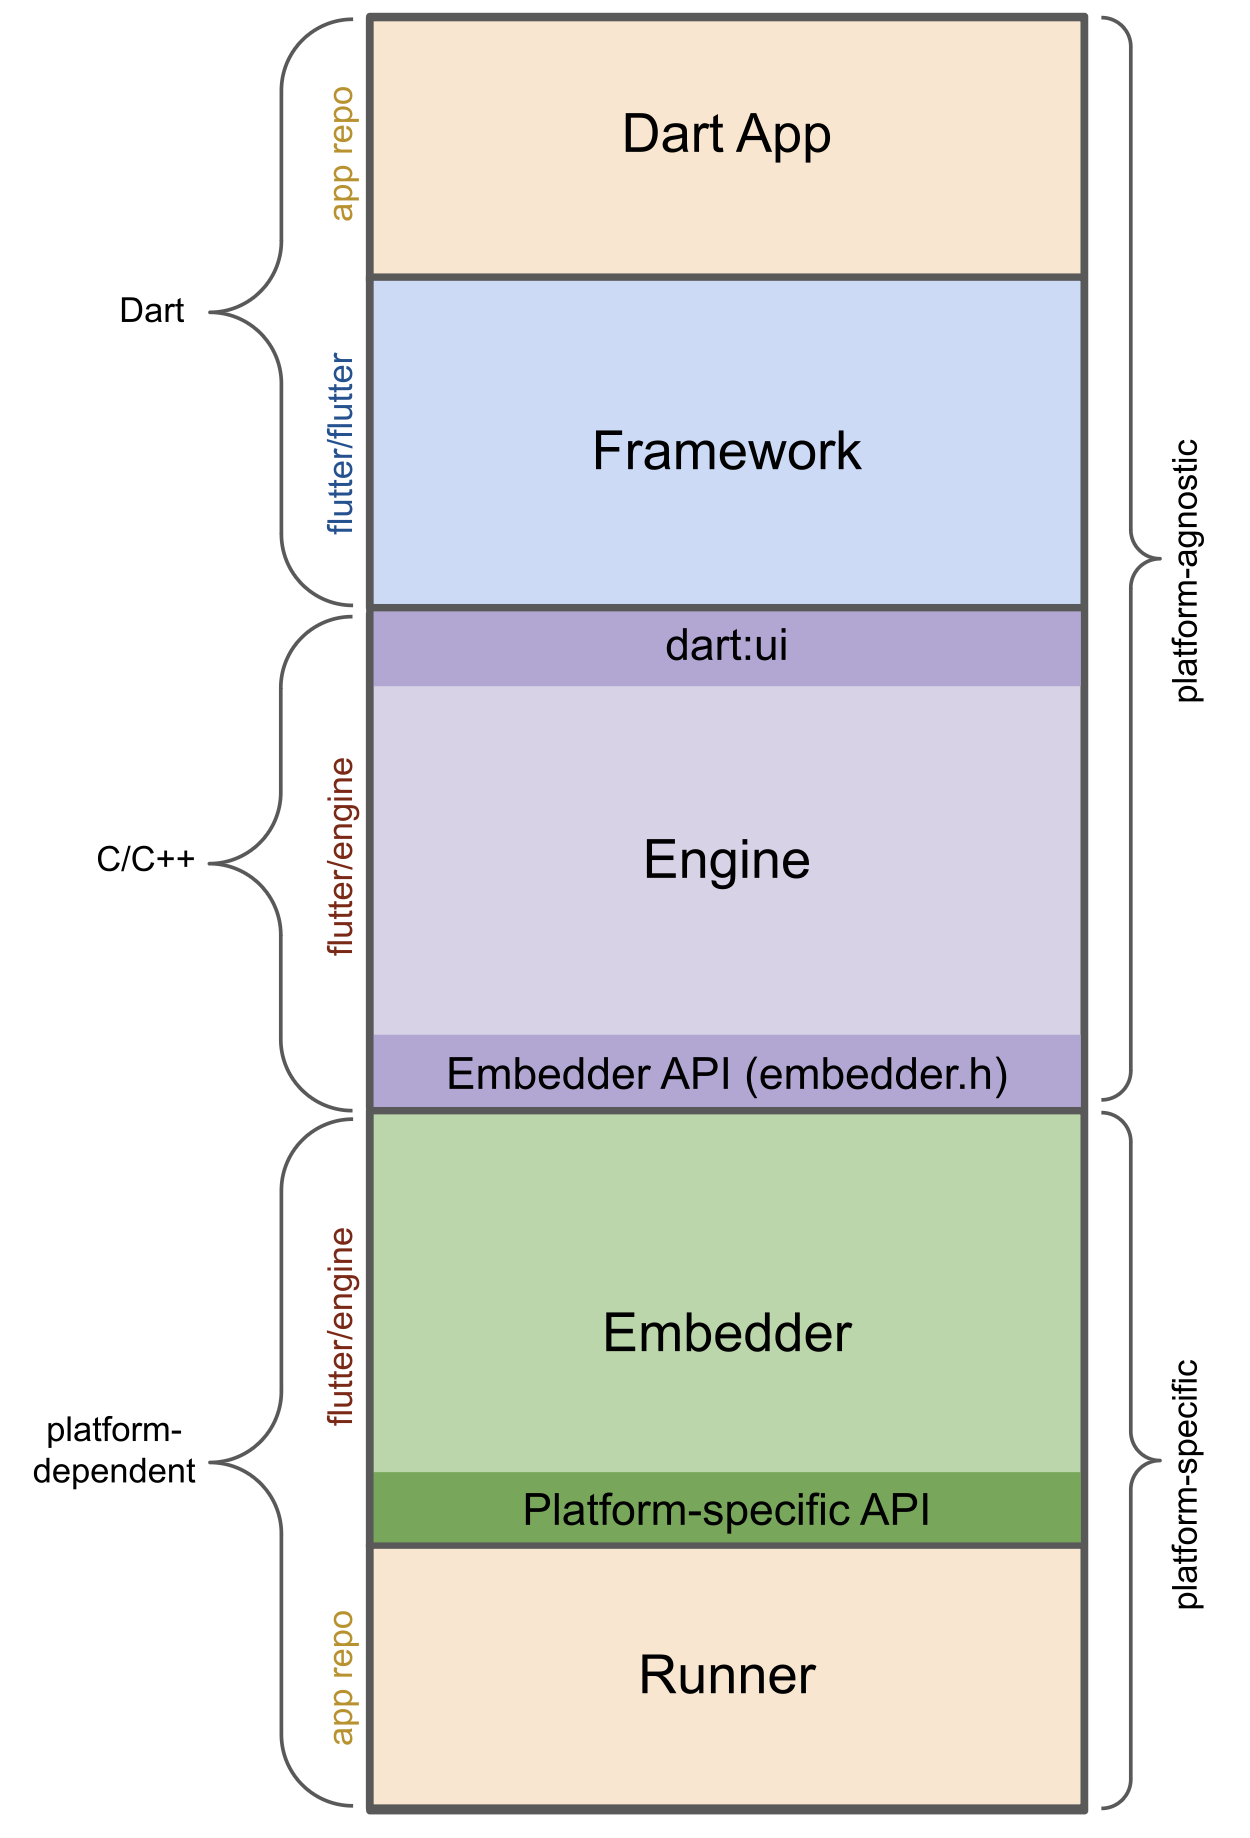
\includegraphics[width=0.4\columnwidth]{images/flutter-app-anatomy.png} 
    \caption{Struttura di un'applicazione in \emph{Flutter}.}
    \label{fig:architettura-flutter}
\end{figure}

Lo stato posseduto dai \lstinline{StatefulWidget} (vedi sezione \ref{subsec:flutter}) può essere considerato come \emph{ephemeral} (ing. effimero) o \emph{app state} (ing. stato dell'applicazione). \\
\emph{Ephemeral} è uno stato che può essere opportunamente confinato all'interno di un singolo \emph{widget} e gestito attraverso la primitiva \lstinline{setState()}, che permette di definire come aggiornarlo.\\
Mentre \emph{app state} è uno stato che viene condiviso tra più \emph{widget} e per la sua gestione, più complessa utilizzando solamente la primitiva sopra citata, esistono diverse librerie di terze parti, ciascuna con le proprie peculiarità a seconda del caso d'uso.\\
\indent La problematica di come gestire lo stato dell'applicazione è definito in gergo \emph{state management}\cite{site:flutter-state-mgmt}, e dopo un'attenta analisi delle librerie disponibili, si è scelto di utilizzare \emph{Riverpod}\cite{site:riverpod}.\\

\subsection{Riverpod}
\label{subsec:riverpod}
% cos'è
% come funziona
% vantaggi
% svantaggi
% motivazione della scelta
\emph{Riverpod} semplifica notevolmente lo \emph{state management} e si basa su un concetto evoluto da \emph{Provider}\cite{site:provider}, libreria da cui deriva.\\
A differenza di \lstinline{InheritedWidget}\cite{site:inheritw} che permette di condividere lo stato tra più \emph{widget}, \emph{Riverpod}, che ne è una reimplementazione, fornisce \emph{providers} che sono indipendenti dai \emph{widget}, in quanto una volta dichiarato il \lstinline{ProviderScope} a livello globale, possono essere richiamati ovunque.\\
Da questo ne consegue che si evita di aggiornare l'interfaccia grafica, ovvero di richiamare il metodo \lstinline{build()} di un \emph{widget} quando non è necessario, poichè è un'operazione costosa.
Un \emph{provider} dunque è un oggetto che può essere richiamato da un \emph{widget} con la finalità di leggerne un valore.\\
Ne esistono di varie tipologie, per le quali si rimanda alla documentazione ufficiale\cite{site:riverpod}, ma quelle utilizzate in questo progetto sono:
\begin{itemize}
    \item \lstinline{FutureProvider}: utilizzato per ricevere un valore generato da un'operazione asincrona (es: richiesta \gls{httpg}\glsoccur);
    \item \lstinline{StateNotifierProvider}: utilizzato per gestire una classe che mantiene uno stato, più complesso di una semplice variabile primitiva, e di esporre dei metodi per monitorarlo o aggiornarlo.
\end{itemize}

\subsection{Architettura dell'applicazione}
\label{subsec:architettura-app}

Per l'architettura dell'applicazione si è scelto di utilizzare un \emph{pattern} architetturale basato su \gls{mvcg}\glsoccur, che permette di separare la logica dell'applicazione dalla sua rappresentazione grafica, in modo da rendere più semplice la manutenzione e l'aggiunta di nuove funzionalità.\\
Nel dettaglio l'applicazione è composta da quattro livelli:
\begin{itemize}
    \item \textbf{Data Layer}: contiene le classi che si occupano di recuperare i dati dal server, attraverso richieste \gls{httpg}\glsoccur, e di convertirli in oggetti rappresentati nel \emph{domain layer};
    \item \textbf{Domain Layer}: contiene le classi che rappresentano i dati dell'applicazione;
    \item \textbf{Application Layer}: contiene le classi che si occupano di gestire la logica dell'applicazione;
    \item \textbf{Presentation Layer}: contiene le classi che si occupano di gestire l'interfaccia, ovvero di eseguire il rendering dei \emph{widget} e di gestire gli eventi generati dall'utente.
\end{itemize}
Questa architettura permette inoltre di avere la possibilità di definire eventualmente più sorgenti da cui recuperare i dati senza dover modificare il codice relativo ai livelli superiori, in quanto è sufficiente modificare il \emph{data layer}\cite{site:app-architecture}.\\

\section{Struttura del progetto}
\label{sec:struttura-progetto}
% Struttura del progetto: cartelle, file, ecc. -> LAYER FIRST
Un altro aspettato importante da considerare per la realizzazione di un progetto software è la sua struttura, ovvero come organizzare i file e le cartelle che lo compongono.\\
Dopo opportune ricerche ed analisi, si è scelto di adottare, tra le due alternative disponibili, la struttura \emph{layer first}, che prevede di organizzare i file e le cartelle in base al livello a cui appartengono, in modo da rendere più semplice la manutenzione e l'aggiunta di nuove funzionalità.\\
\emph{Feature first}, l'altra alternativa, organizza invece i file e le cartelle, mantendendo la separazione tra i livelli, in base alle funzionalità che l'applicazione offre.\\
Il motivo principale per cui la scelta non è ricaduta su quest'ultima è che, nonostante sia quella che garantisca un'organizzazione e manutenzione del codice migliore, risulta essere più complessa da implementare in quanto adatta per progetti di dimensione e complessità maggiore.\\
Di seguito verranno illustrati entrambi gli approcci, in modo da poterli confrontare e comprendere meglio le loro differenze\cite{site:project-structure}.\\
\begin{multicols}{2}
    \begin{verbatim}
        // LAYER FIRST
        lib/
            data/
                feature1.dart
                feature2.dart
            domain/
                feature1.dart
                feature2.dart
            application/
                feature1.dart
                feature2.dart
            presentation/
                feature1.dart
                feature2.dart
    \end{verbatim}
    \begin{verbatim}
        // FEATURE FIRST
        lib/
            feature1/
                data.dart
                domain.dart
                application.dart
                presentation.dart
            feature2/
                data.dart
                domain.dart
                application.dart
                presentation.dart
    \end{verbatim}
\end{multicols}

% \section{Diagrammi UML}
% \label{sec:uml}
% dove inserirli?
% UML -> Diagrammi delle classi

% \subsubsection{Namespace 1} %**************************
% Descrizione namespace 1.

% \begin{namespacedesc}
%     \classdesc{Classe 1}{Descrizione classe 1}
%     \classdesc{Classe 2}{Descrizione classe 2}
% \end{namespacedesc}

\section{Ambiente di sviluppo}
\label{sec:ambiente-sviluppo}
% SEGUI ISSUE #4 E #5 PER LA STESURA DI QUESTA SEZIONE
Di seguito viene descritto l'ambiente di sviluppo e data una panoramica delle tecnologie e strumenti utilizzati.

\subsection*{Figma}
\label{subsec:figma}

\emph{Figma}\cite{site:figma} è un software di editor di grafica vettoriale che permette di progettare interfacce grafiche per applicazioni \emph{web} e \emph{mobile}.\\
È stato utilizzato per la realizzazione del \gls{mockup}\glsoccur dell'applicazione, in quanto vi è la possibilità di creare un prototipo interattivo, che simula l'interazione dell'utente con l'applicazione, e di condividerlo con il team di sviluppo, in modo da avere un'idea più chiara di come l'applicazione debba essere strutturata e di come debba funzionare.\\

\subsection*{Git}
\label{subsec:git}

\emph{Git}\cite{site:git} è un sistema di controllo di versione, finalizzato al tracciamento del codice sorgente e delle sue modifiche, inoltre ne permette la condivisione e dunque la collaborazione tra più sviluppatori.\\
Inoltre è possibile, eventualmente, in caso di errori, di poter ripristinare una versione precedente del codice sorgente.\\

\subsection*{GitHub}
\label{subsec:github}

% DA DEFINIRE: ISSUE, MILESTONE
\emph{GitHub}\cite{site:github} è un servizio di hosting per il codice sorgente di progetti software che utilizza \emph{Git}.\\
Per questo progetto è stato utilizzato per la condivisione e gestione del codice sorgente attraverso una repository dedicata, fornita dall'azienda.\\
Per la pianificazione della fase di implementazione è stato utilizzato il sistema di \gls{issuetracking}\glsoccur integrato, creando delle \gls{milestone}\glsoccur per ogni classe di obbiettivi da raggiungere in base alla loro priorità (vedi sezione \ref{sec:obiettivi}).\\
In ciascuna \gls{milestone}\glsoccur sono state create delle \emph{issue}, in base ai requisiti o ad un insieme di questi, necessarie per il raggiungimento di ciascun obbiettivo, garantendo così una maggiore organizzazione e tracciabilità del lavoro svolto e dei progressi fatti.\\

\subsection*{VSCode}
\label{subsec:vscode}

Editor di codice sorgente \gls{open-source}\glsoccur che oltre a fornire le funzionalità di base necessarie per lo sviluppo (ad esempio: controllo di sintassi, \emph{debugging}, analisi statica del codice, ecc.), supporta molti linguaggi di programmazione ed è possibile estendere le sue funzionalità o il numero di linguaggi supportati attraverso delle estensioni.\\
Di fatto per questo progetto si è reso necessario l'installazione di alcune estensioni, tra cui:
\begin{itemize}
    \item \textbf{Flutter}\cite{site:flutter-extension};
    \item \textbf{Dart}\cite{site:dart-extension}.
\end{itemize}

\subsection*{Flutter}
\label{subsec:flutter}

\emph{Flutter}\cite{site:flutter} è un \gls{framework}\glsoccur che consente di sviluppare applicazioni native per diverse piattaforme, come Android, iOS, web e desktop, utilizzando un unico linguaggio di programmazione, riducendo i tempi e i costi di produzione, senza compromettere le prestazioni dell'applicazione.\\
Il concetto centrale di \emph{Flutter} è quello dei \emph{widget}, oggetti che descrivono come deve essere visualizzata una parte dell'interfaccia grafica. Questi possono essere di due tipi:
\begin{itemize}
    \item \textbf{StatelessWidget}: non hanno uno stato interno, ovvero non cambiano nel tempo, e sono definiti da un insieme di proprietà, chiamate \emph{proprietà immutabili}, che vengono passate al costruttore del \emph{widget};
    \item \textbf{StatefulWidget}: al contrario, possiedono uno stato interno mutabile, e viene usato quando una parte dell'interfaccia utente può cambiare dinamicamente.
\end{itemize}

\subsection*{StarUML}
\label{subsec:staruml}

\emph{StarUML}\cite{site:staruml} è uno strumento di modellazione per sistemi software che sono sviluppati secondo il paradigma \emph{orientato agli oggetti}, attraverso la creazione di diagrammi \gls{umlg}\glsoccur.\\
È stato utilizzato per la realizzazione dei casi d'uso (vedi sezione \ref{sec:usecase}) e dei diagrammi delle classi.\\

\subsection*{Emulatori Android e iOS}
\label{subsec:emulatori}

Per testare l'applicazione su dispositivi \emph{Android} e \emph{iOS} è stato utilizzato rispettivamente \emph{Android Studio}\cite{site:android-studio} e \emph{Xcode}\cite{site:xcode}, che forniscono degli emulatori per le rispettive piattaforme.\\

A completare l'ambiente di sviluppo, l'azienda mi ha fornito l'accesso alle \gls{apig}\glsoccur del loro \gls{backend}\glsoccur attraverso lo \emph{Swagger}\cite{site:swagger}, strumento che, tra le altre cose, consente di consultare la documentazione delle \gls{apig}\glsoccur e di testarle attraverso un'interfaccia grafica \emph{web}.\\
Si specifica che per lo sviluppo dell'applicazione, l'utilizzo di tali \gls{apig} è stato svolto su un \emph{server} di collaudo.
    \chapter{Conclusioni}
\label{cap:conclusioni}

\intro{In questo ultimo capitolo verranno illustrati gli obiettivi raggiunti, il consuntivo delle attività e infine verrà fornita una valutazione personale sul tirocinio svolto.}\\

\section{Obiettivi raggiunti}
\label{sec:raggiungimento-obiettivi}

La Tabella \ref{tab:obbiettivi-raggiunti} illustra gli obiettivi raggiunti al termine del tirocinio.

\begin{table}
    \centering
    \begin{tabular}{|l|l|l|}
        \hline
        \textbf{Obiettivo} & \textbf{Priorità} & \textbf{Stato} \\ \hline
        \hyperref[O01]{O01}                & Obbligatorio      & Soddisfatto    \\ \hline
        \hyperref[O02]{O02}                & Obbligatorio      & Soddisfatto    \\ \hline
        \hyperref[O03]{O03}                & Obbligatorio      & Soddisfatto    \\ \hline
        \hyperref[O04]{O04}                & Obbligatorio      & Soddisfatto    \\ \hline
        \hyperref[O05]{O05}                & Obbligatorio      & Soddisfatto    \\ \hline
        \hyperref[D01]{D01}                & Obbligatorio      & Soddisfatto    \\ \hline
        \hyperref[D02]{D02}                & Obbligatorio      & Non soddisfatto    \\ \hline
        \hyperref[F01]{F01}                & Obbligatorio      & Non soddisfatto    \\ \hline
    \end{tabular}%
\caption{Tabella con gli obiettivi raggiunti}
\label{tab:obbiettivi-raggiunti}
\end{table}

\noindent Il mancato soddisfascimento degli obiettivi \emph{D02} e \emph{F01}, ovvero il \emph{deploy} e la stesura dei test per la verifica e validazione dell'applicazione, è stato causato principalmente dalla mancanza di tempo. \\
Come evidenziato dal reale svolgimento delle attività (Sezione \ref{subsec:variazione-pianificazione}), la fase di sviluppo è stata più lunga del previsto.\\
Malgrado non siano stati progettati e scritti i test per la verifica e validazione dell'applicazione, si è comunque cercato di mantenere un codice pulito e ben strutturato, in modo da facilitare eventuali modifiche e manutenzioni future, anche se come garanzia di qualità non può considerarsi sufficiente.
Si specifica, inoltre, che la verifica delle funzionalità dell'applicazione è stata effettuata dal tutor aziendale o da altri colleghi, lungo tutto il periodo di sviluppo del progetto, fornendo un \emph{feedback} immediato, permettendo così di apportare eventuali modifiche correttive e miglioramenti.\\
Per quanto riguarda il \gls{deploy}\glsoccur, il principale motivo per cui non è stato effettuato, è da imputarsi al fatto che l'utenza a cui è rivolta l'applicazione è molto ristretta, risultava quindi superfluo e non necessario pubblicarla sulle piattaforme \emph{Google Play Store} e \emph{Apple App Store}. Tale decisione è stata presa dal tutor aziendale che ha ritenuto più opportuno pensare ad un modo alternativo per distribuire l'applicazione direttamente agli utenti finali.

\section{Consuntivo delle attività}
\label{sec:consultivo-attivita}

Sulla base di quanto descritto nella Sezione \ref{sec:raggiungimento-obiettivi}, la Tabella \ref{tab:consultivo-ore} riporta la differenza tra le ore pianificate (presenti nel documento \emph{Piano di lavoro}) ed effettive per ogni attività del tirocinio.

\begin{table}
    \centering
    \begin{tabularx}{\textwidth}{|c|c|X|}
        \hline
        \textbf{Ore effettive} & \textbf{Ore pianificate} & \textbf{Descrizione dell'attività} \\\hline
        
        \textbf{70} & \textbf{80} & \textbf{Formazione sulle tecnologie} \\	 
        \hline
        
        \textbf{40} & \textbf{40} & \textbf{Definizione architettura di riferimento e relativa documentazione} \\ \hdashline 
        \multirow{3}{0cm}\\ 
        \textit{14} &
        \textit{12} & 
        \textit{Analisi del problema e del dominio applicativo} \\
        \textit{20} &
        \textit{22} & 
        \textit{Progettazione della piattaforma e relativi test} \\
        \textit{6} &
        \textit{6} & 
        \textit{Stesura documentazione relativa ad analisi e progettazione} \\
        \hline
        

        \textbf{192} & \textbf{160} & \textbf{Sviluppo}  \\ \hdashline 
        \multirow{5}{0cm}\\ 
        \textit{40} &
        \textit{26} & 
        \textit{Implementazione del meccanismo di autenticazione e integrazione con il sistema preesistente per il prelevamento dei dati da visualizzare nell'applicazione} \\
        \textit{40} &
        \textit{34} & 
        \textit{Implementazione delle funzionalità di creazione e compilazione (testuale e vocale) delle meeting-note} \\
        \textit{40} &
        \textit{28} & 
        \textit{Integrazione del servizio OpenAI} \\
        \textit{24} &
        \textit{40} & 
        \textit{Attività di testing} \\
        \textit{48} &
        \textit{32} & 
        \textit{Sviluppo UI} \\
        \hline
        
        \textbf{10} & \textbf{40} & \textbf{Verifica e Validazione finale}  \\ \hdashline 
        \multirow{3}{0cm}\\ 
        \textit{0} &
        \textit{24} & 
        \textit{Esecuzione dei test per la verifica e collaudo dell'applicazione} \\
        \textit{10} &
        \textit{8} & 
        \textit{Stesura documentazione finale} \\
        \textit{0} &
        \textit{8} & 
        \textit{Deploy dell'applicazione} \\
        \hline
        
        \textbf{Totale ore} & \multicolumn{1}{|X|}{\textbf{312}} \\ 
        \hline
        
    \end{tabularx}
    \caption{Consuntivo della durata delle attività}
    \label{tab:consultivo-ore}
\end{table}

\section{Valutazione personale}
\label{sec:valutazione-personale}

Il tirocinio è stato un'esperienza molto formativa, in quanto mi ha permesso di mettere in pratica le conoscenze e metodologie acquisite durante il percorso di studi in un contesto lavorativo.\\
Come già menzionato in precedenza, nonostante la mia familiarità con alcune delle tecnologie adottate, ho avuto modo di approfondirle e di imparare nuovi concetti, soprattutto per quanto riguarda il \emph{framework} \emph{Flutter}.\\
Inoltre, per la prima volta ho avuto modo di lavorare ad un progetto in maniera più professionale, seguendo anche alcuni principi affrontati durante il corso di \emph{Ingegneria del Software}, come ad esempio la pianificazione della fase di sviluppo, fissando delle \gls{milestone}\glsoccur, mantenendo traccia dei progressi per il raggiungimento degli obiettivi del progetto, e la documentazione del codice, in modo da rendere più facile la comprensione e la manutenzione del codice.\\  
L'azienda mi ha lasciato molta autonomia durante lo sviluppo del progetto e mi ha fornito un \emph{feedback} costante, permettendomi di migliorare e di imparare nuove cose. \\
In conclusione, ritengo che il tirocinio sia stato un'esperienza molto positiva, che mi ha permesso di crescere sia dal punto di vista professionale che personale.

    \appendix
    \chapter{Appendice A}

\epigraph{Citazione}{Autore della citazione}


    \backmatter
    \printglossary[type=\acronymtype, title=Acronimi e abbreviazioni, toctitle=Acronimi e abbreviazioni]
    \printglossary[type=main, title=Glossario, toctitle=Glossario]

    \cleardoublepage
\chapter{Bibliografia}

% \nocite{*}

% Print book bibliography
\printbibliography[heading=subbibliography,title={Riferimenti bibliografici},type=book]

% Print site bibliography
\printbibliography[heading=subbibliography,title={Siti web consultati},type=online]

\end{document}
